\documentclass[12pt]{report} 

\usepackage[language=english, type=bachelor]{style}
\usepackage{subfigure}
\usepackage{fancyhdr}
\pagestyle{fancy}
\usepackage[T1]{fontenc}
\usepackage[utf8]{inputenc}
\usepackage{array,multirow,graphicx}
\usepackage{color}
\usepackage{float}
\usepackage[table]{xcolor}
\usepackage{url}
\lhead{}
\chead{}
\renewcommand{\headrulewidth}{0.2pt}
\renewcommand{\footrulewidth}{0.2pt}

\begin{document}

\specialization{INFORMATIC\u{A} ROM\^{A}N\u{A}}	
\title{MammoDetect: Deep Learning Techniques for Breast Cancer Detection: A Comparative Study of GoogLeNet and EfficientDet in 3D Imaging}					   
\author{Baciu Ioana}											
\supervisor{prof. Dio\c san Laura}				
				
\maketitle


\newpage
\thispagestyle{empty}
\mbox{}
\newpage
\pagenumbering{roman} 

\cleardoublepage
ABSTRACT
\vspace{0.5cm}	
\hrule
\vspace{0.5cm}	




The purpose of this thesis is to experiment and compare how a GoogLeNet architecture will perform in classifying breast images into normal or cancerous. Along with the classification problem, a second model representing an EfficientDet architecture focused on detecting the tumors in the aforementioned images and also classifying them into benign or malign. The best performing models from each problem have been selected and integrated into an intelligent system that aims to showcase the use of the two models in real life scenarios. 

In order to get the best configuration for each architecture I conducted many experiments on each one and documented them in chapter \ref{chap:ch4}. The detailed description of the architecture structure for both GoogLeNet and EfficientDet have been written in chapter \ref{chap:ch3}. Other ways of solving breast cancer classification and detection are presented in chapter \ref{chap:ch2}. Chapter \ref{chap:ch5} explains the evolution of the system and finally, chapter \ref{chap:ch6} encompass the conclusions of the thesis and how to improve the performance of the models resulted after the experiments.

\tableofcontents


\newpage
\pagenumbering{arabic}

\chapter{Introduction}

\label{intro}

\par Breast cancer is known to be the most common cancer among women~\cite{link1}. The American Cancer Society’s estimates for breast cancer in the United States alone for 2023 are that about 297,790 new cases of invasive breast cancer will be diagnosed in women and about 43,700 women will die from breast cancer~\cite{link2}. Since 1989, breast cancer death rates have been decreasing, believed to be a consequence of early detection and increased awareness, as well as better treatments. This progress seems to have slightly stopped~\cite{link2}.\\
The main objective of this project is to understand and implement ways to detect the presence of cancerous, benign, or precancerous tumors in the breast in an efficient way using machine learning. This would minimize the time doctors spend studying thousands of breast screenings to label them accordingly and aid early detection.

\chapter{Existing methods of detecting breast cancer}
\label{chap:ch2}

\par There are several articles related to studying various ways of implementing breast cancer detection using machine learning. There is “Machine Learning Techniques for Breast Cancer Prediction” by Varsha Nemade and Vishal Fegade from Mukesh Patel School of Technology Management and Engineering, NMIMS Shirpur Campus, India~\cite{carte2}. They have documented different ML classification techniques and evaluated each of them using different performance measures, such as accuracy, precision, and recall. These techniques include N{\"a}ive Bayes, Logistic Regression, Support Vector Machine, K-Nearest Neighbour and Decision Tree, the latter being found to have the highest accuracy, 97\%.

The dataset used in their experiments was the WDBC dataset, which contains features from 569 digitized images of a fine needle aspirate of a breast mass~\cite{link3}. The algorithm implemented uses features from the image rather than the image itself, some of which include radius, texture, area, perimeter, smoothness, compactness, concavity, concavity points, symmetry and fractal dimension. The following charts represent the performance of the classification techniques used.

\begin{figure}[h!]
    \centering
    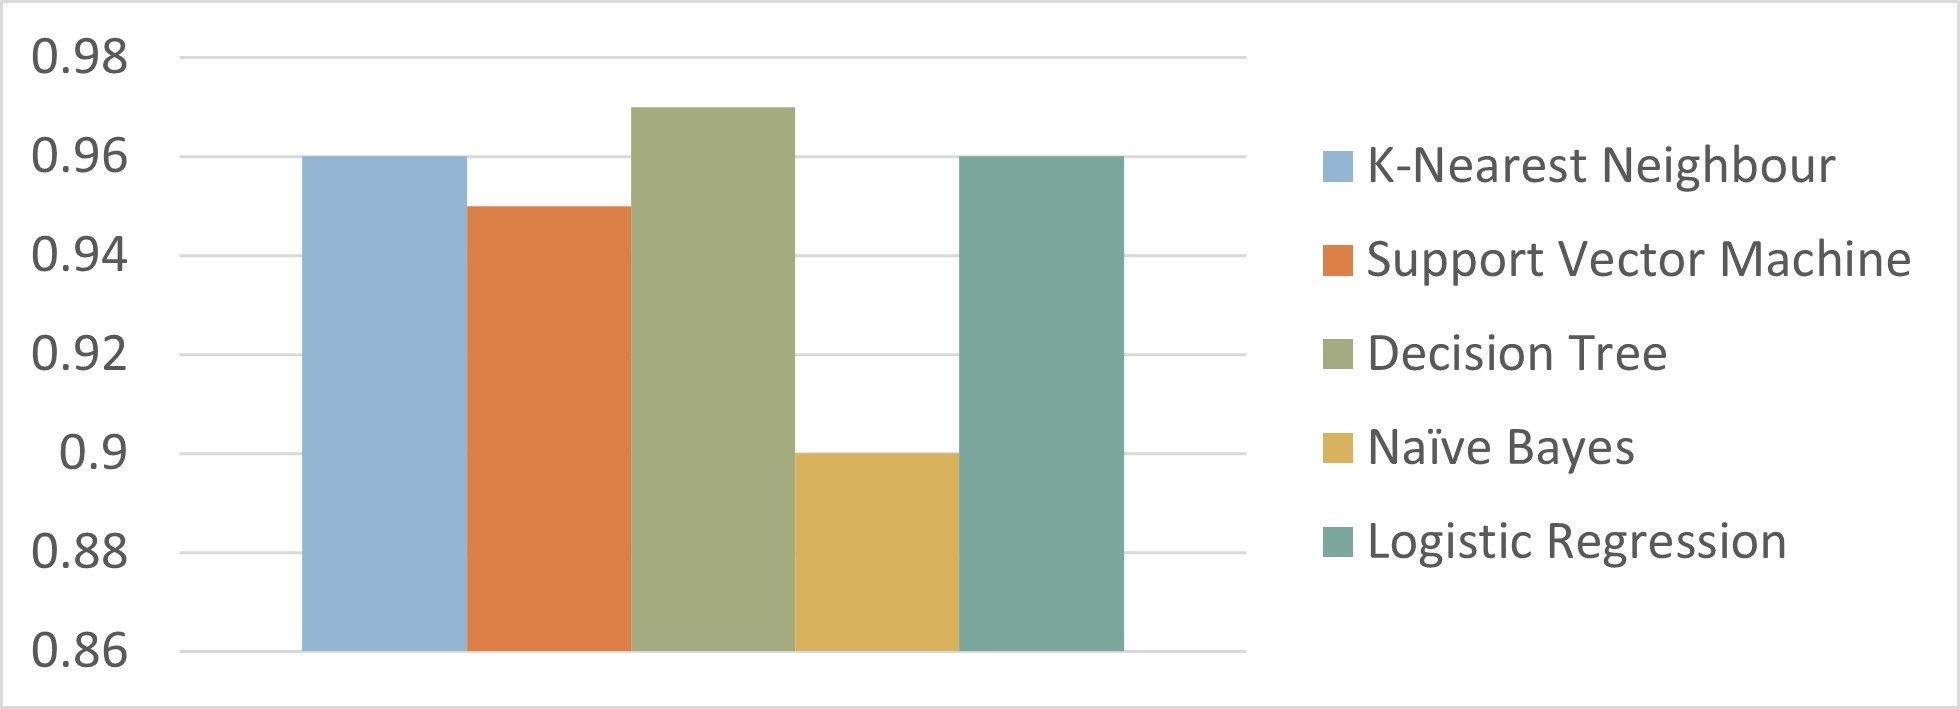
\includegraphics[width=0.75\textwidth]{figures/Figure1.jpg}
    \caption{Accuracy of classification techniques}
    \label{fig:fig1}
\end{figure}
\begin{figure}[h!]
    \centering
    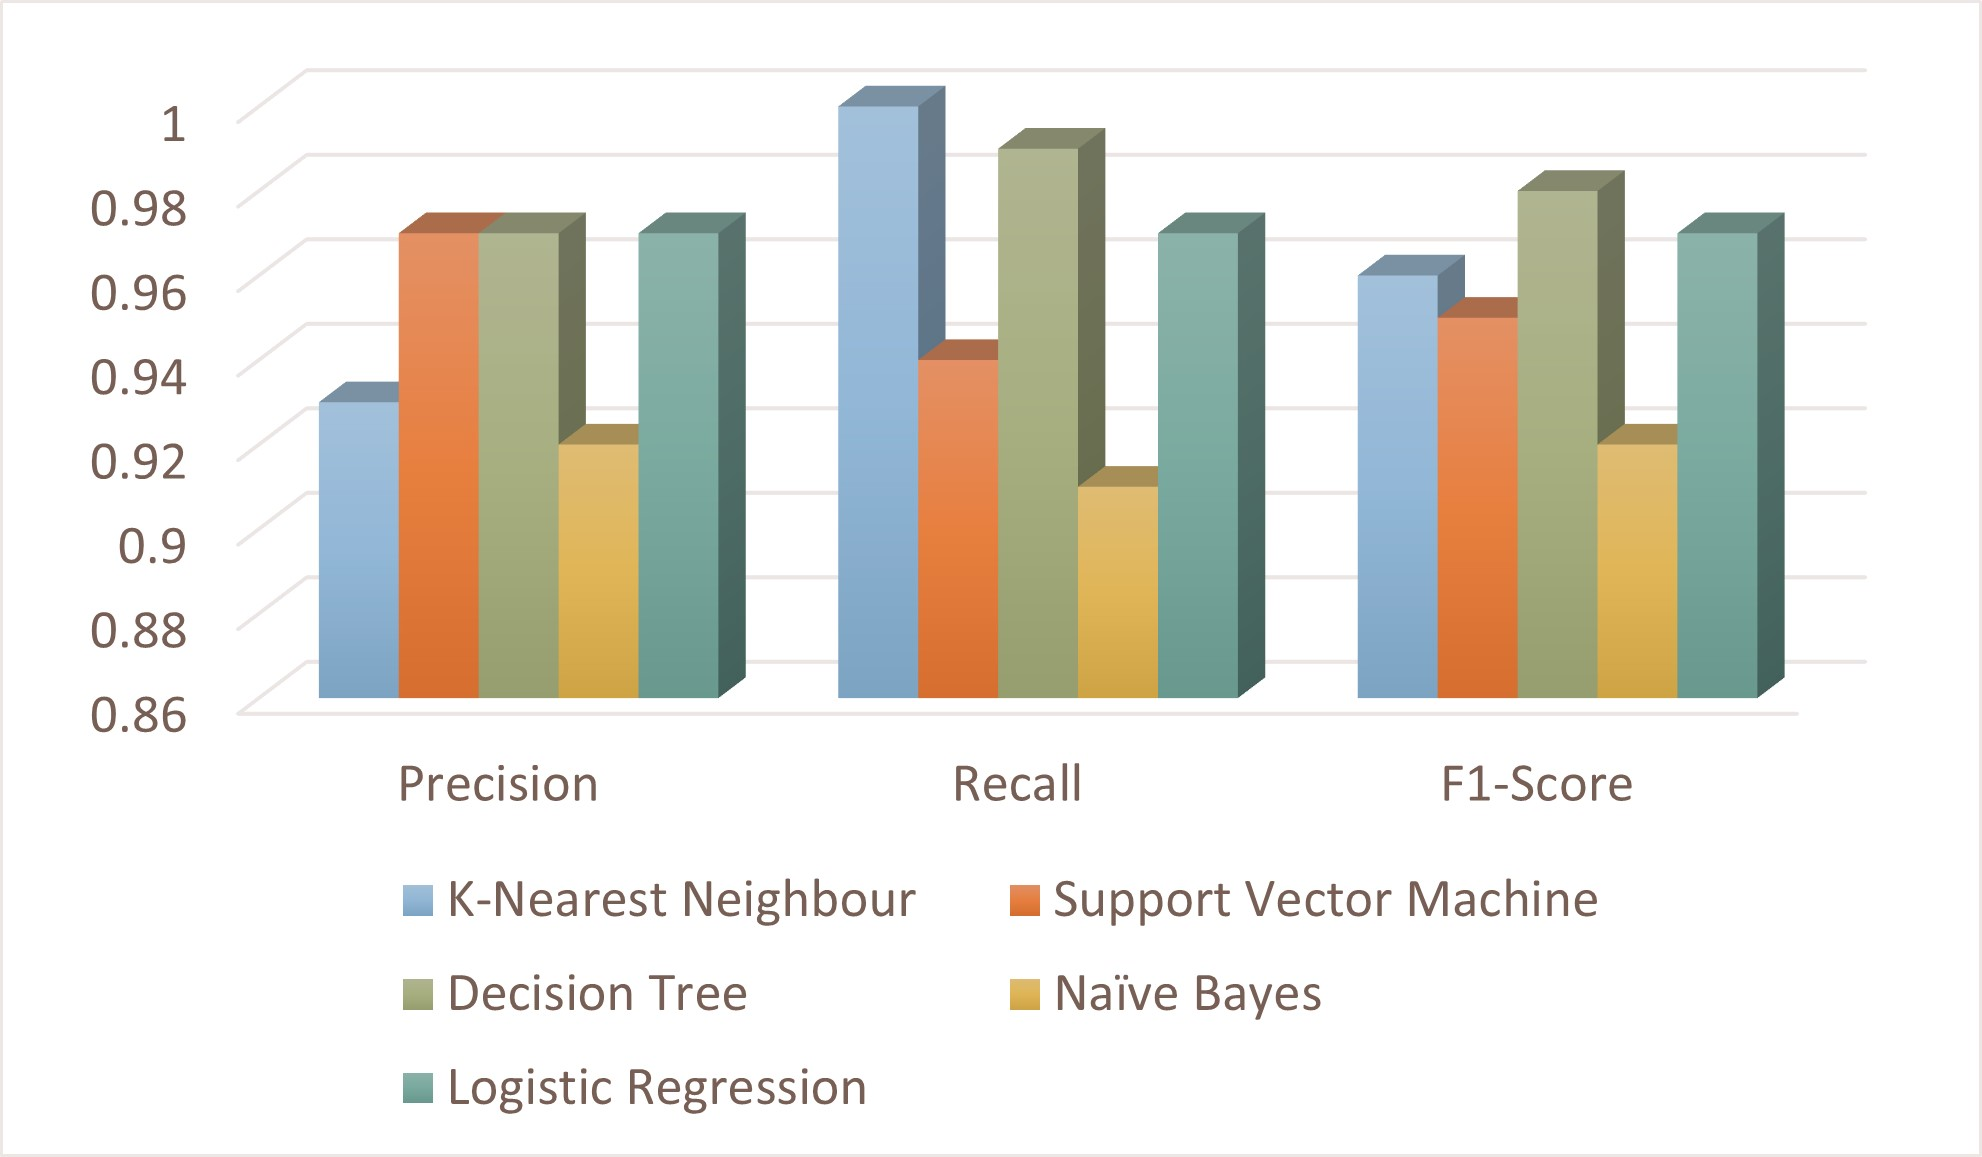
\includegraphics[width=0.75\textwidth]{figures/Figure2.jpg}
    \caption{Performance of classification techniques for class benign}
    \label{fig:fig2}
\end{figure}
\begin{figure}[h!]
    \centering
    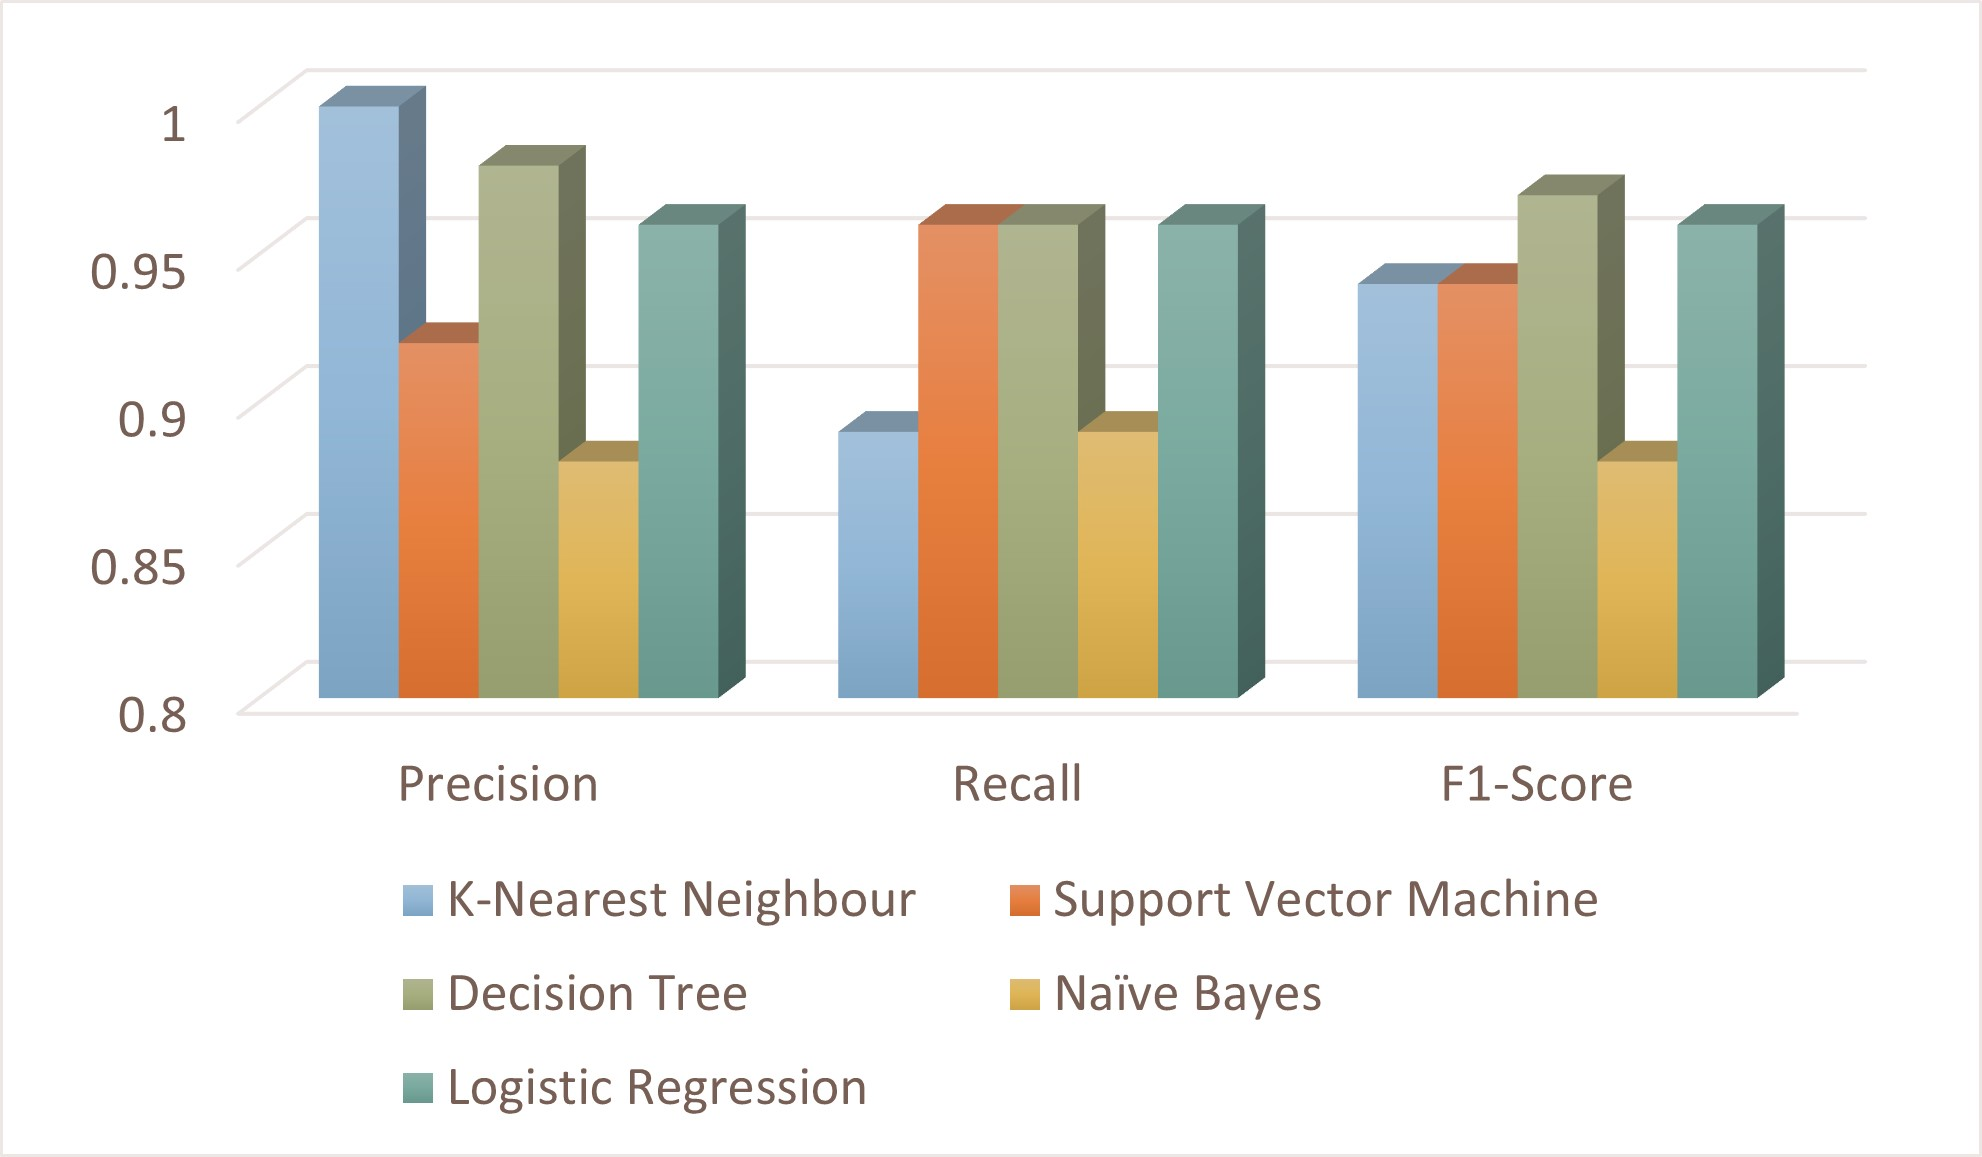
\includegraphics[width=0.75\textwidth]{figures/Figure3.jpg}
    \caption{Performance of classification techniques for class malignant}
    \label{fig:fig3}
\end{figure}

Other relevant studies include “An enhanced Predictive heterogeneous ensemble model for breast cancer prediction” concluded by S. Nanglia et al. which got 78\% accuracy using KNN, SVM and DT~\cite{carte1}. Islam et al. got a 98.75\% using ANN on the WDBC~\cite{carte3}. Amrane et al. proposed an approach using KNN and NB with 97.51\% accuracy~\cite{carte4}. Dhahri et al. studied the usage of genetic programming techniques for the selection of the best features and parameters for the machine learning classifier~\cite{carte5}.
\chapter{Backgrounds in classification and detection architectures}
\label{chap:ch3}

In the interest of improving image classification, there have been many models documented, each trying to be better than the previous ones. The most commonly used include ResNet, DenseNet, VGGNet, AlexNet and GoogLeNet ~\cite{link8}. The same can be said about detection models; some of the most popular in 2024 are YOLO (You Only Look Once), RetinaNet, Faster-RCNN and EfficientDet~\cite{carte11}.

Of all of these models, I chose to integrate into my system GoogLeNet for classification and EfficientDet for detection.

\section{GoogLeNet}
This models first appereance was in an research paper published in 2014 called "Going Deeper with Convolutions"
\textcolor{green}{please add a ref - see this ref \href{https://arxiv.org/abs/1409.4842}{link}}
. The researches at Google, along with other universities, received that year the first place in the  ILSVRC 2014 image classification competition, by achieving a less error rate than the other contestants. They managed this by introducing new concepts, such as 1x1 convolution, global average pooling, inception module and auxiliary classifiers.
\textcolor{green}{eu as aduaga aici cateva info despre arhitectura (sau o poza, ca sa se vada layerele) si despre cum se face trainingul (de exemplu, cum se calculeaza loss-ul, cum se face backpropagation, etc., ce inseamna acel InceptionBloc care e un element vital in deep learning)}

\section{EfficientDet Architecture}

The EfficientDet model is a new family of object detectors based on two main optimizations, those being efficient multi-scale feature fusion and model scaling. Along with those optimizations, different models have been tested to serve as the backbone of the model, and for this particular model, EfficientNet has proven to be a sufficient backbone architecture~\cite{carte8}.

The first challenge of this model was feature fusion, a concept introduced to aid convolutional neural networks in identifying objects from images when the objects' sizes are either too small or exceed the convolutional kernel's receptive field.~\cite{carte9}. It has been discovered that changing the resolution of the image solved the sensitivity that neural networks have to the images' size, to some extent, as shown in figure \ref{fig:fig4}.

\begin{figure}[!ht]
    \centering
    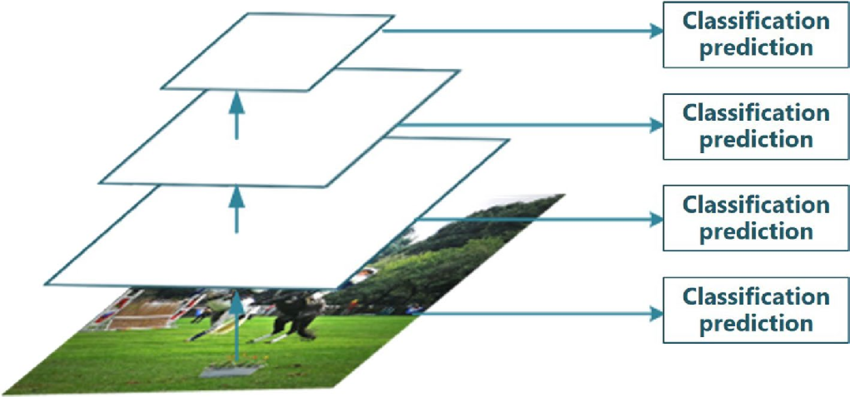
\includegraphics[width=0.7\textwidth]{figures/Figure4.png}
    \caption{Pattern diagram of image pyramid, obtained from ~\cite{link13}}
    \label{fig:fig4}
\end{figure}

The problem with this discovery was that the cost of system storage for creating a pyramid of the same image in different resolutions and computational resources are too harsh, therefore deeming this method rarely usable. Because each resolution had its advantages, a way to combine features from high-resolution features of shallow networks with the high-level semantic information of high-level network features was researched. Thus, the FPN, or Feature Pyramid Network, has been used to extract from deep-layer networks and get the same features as the shallow-layer features by up-sampling, as shown in figure \ref{fig:fig5}. 

\begin{figure}[!ht]
    \centering
    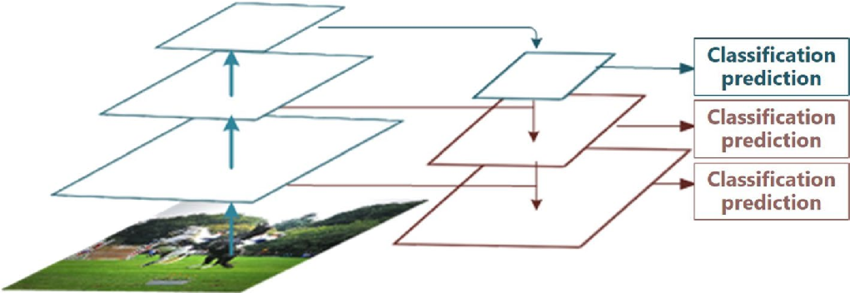
\includegraphics[width=0.7\linewidth]{figures/Figure5.png}
    \caption{Pattern diagram of feature pyramid network, obtained from ~\cite{link12}}
    \label{fig:fig5}
\end{figure}

In this particular model, a BiPFN has been introduced, Bi-directional FPN, which utilizes learnable weights to learn the importance of different input features from different resolutions.

The second challenge is model-scaling. This method was popularized in \cite{carte10}, and is used to uniformly scale all dimensions of depth, width and resolution using a compound coefficient. This scaling method, called compound scaling, is looking at how the different dimensions interact with each other and scales them accordingly. For the EfficientDet architecture, this scaling method is used to scale up resolution, width and depth for all layers of the backbone, BiFPN and the bounding boxes and classification network.

Finally, for the backbone, EfficientNet has been observed to achieve better accuracy than other previously used backbones ~\cite{carte8}. 
% \subsubsection{Bi-directional Feature Pyramid Network}
The baseline strategy for a standard FPN is to aggregate the features from the different levels of resolution in a top-down manner, from the features of the image with the lowest resolution to the ones from the highest one. For example, if a feature is extracted from the lowest resolution image, that feature is passed through a convolutional layer, used for feature processing, and the resulting output is then resized, which could be upsampling or downsampling in order to match the resolution of the following feature and so on ~\cite{carte8}.

The conventional FPN is, however, limited by the one-directional feature flow. To correct this use, PANet, or Path Aggregation Network, is introduced and adds a path going bottom-up. These methods are still not ideal because of the cost of computations and parameters needed. The strategy proposed in \cite{carte8} says that nodes that have only one edge going into them should be removed because the lack of multiple input edges corresponds to less contribution to the overall feature network as it does not involve feature fusion. Moreover, between every input and output node at the same level, there are edges added in order to add more feature fusion without much cost, as it is on the same level. Finally, each bidirectional path is treated as one singular layer and more layers are involved in order to achieve more high-level feature fusion, as shown in figure \ref{fig:fig6}.

\begin{figure}[!ht]
    \centering
    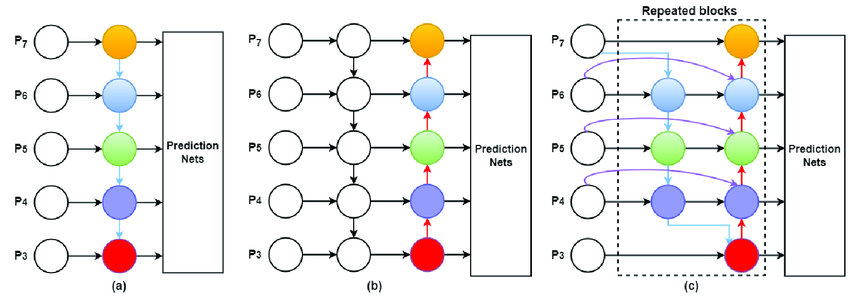
\includegraphics[width=1\textwidth]{figures/Figure6.png}
    \caption{(a)-Conventional FPN; (b)-PANet; (c)-BiFPN, obtained from ~\cite{link14}}
    \label{fig:fig6}
\end{figure}

In addition to the bidirectional cross-scale connections, the EfficientDet model takes into consideration the importance of the different features at different resolutions that can impact the predictions. Therefore, it implements a weighted feature fusion, or more precisely, a fast normalized fusion, that does not affect the performance of the GPU while also maintaining training stability~\cite{carte8}.
% \subsubsection{Conclusion}
Thus, the EfficientDet model combines all these concepts into a singular network, using ImageNet pretrained weights for the EfficientNet model, the BiFPN levels, that take the features from levels 3 to 7 from the backbone and applies feature fusion. In the end, these features are sent to a classification head and a regression head to both classify the objects detected and provide bounding boxes for them. Below is shown the EfficientDet architecture (see Figure \ref{fig:fig7}).

\begin{figure}[!ht]
    \centering
    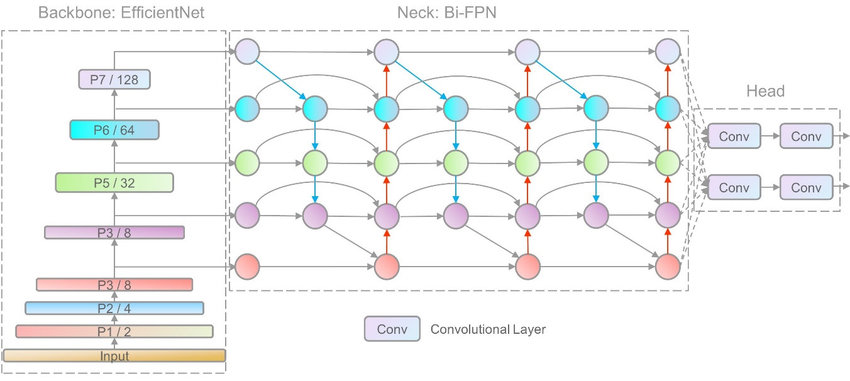
\includegraphics[width=1\textwidth]{figures/Figure7.jpg}
    \caption{EfficientDet architecture, obtained from ~\cite{link15}}
    \label{fig:fig7}
\end{figure}

\chapter{Experimental results obtained}
\label{chap:ch4}

The figure \ref{fig:fig33} below shows the pipeline of the system and how the image flows from the classification model to the detection model.

\begin{figure}[H]
    \centering
    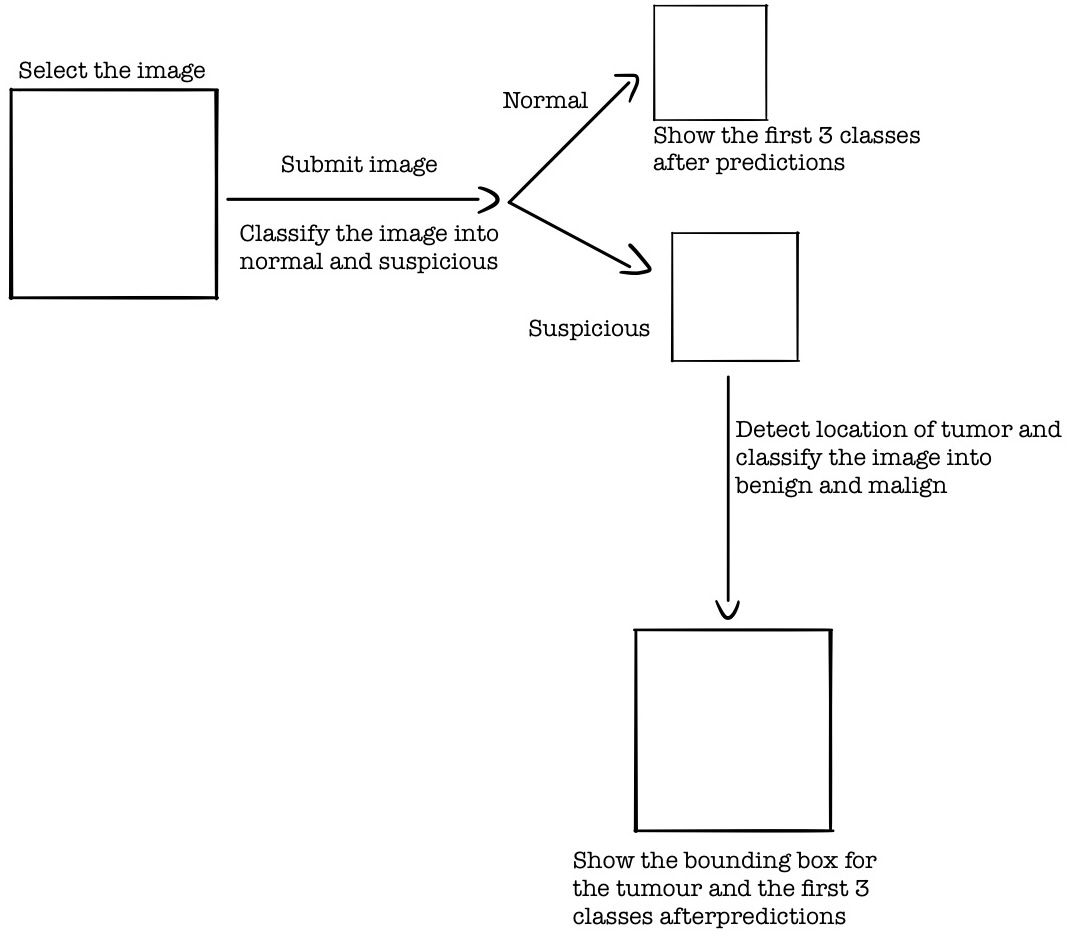
\includegraphics[width=0.7\linewidth]{figures/Figure38.png}
    \caption{System flow}
    \label{fig:fig33}
\end{figure}

\section{Breast Cancer Screening}

The purpose of this thesis is to test the accuracy and precision resulting from training a GoogLeNet model on the Breast-Cancer-Screening-DBT database~\cite{link4}. From this database, only a part of the data has been selected for training and validation. Thus, the database I will be working on contains 719 screenings, of which 350 don't present any cancer, 280 have actionable skin neoplasms, 42 have benign tumors and 47 show signs of malignant cancerous tumors. Figure \ref{fig:fig30} shows the distribution of the classes.

\begin{figure}[hb!]
    \centering
    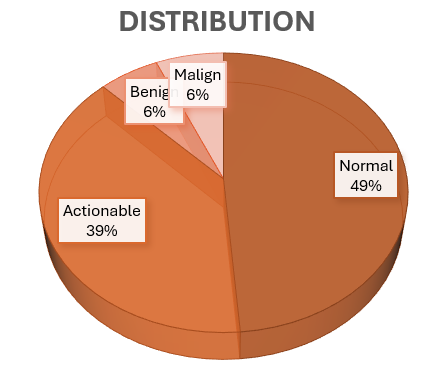
\includegraphics[width=0.5\linewidth]{figures/Figure36.png}
    \caption{Distribution of the classes of the Breast Cancer Screening DBT database among the 719 inputs}
    \label{fig:fig30}
\end{figure}

The Cancer Imaging Archive site provides a download link to a .tcia file that contains the screening files, which can be further downloaded using the NBIA Data Retriever. The images come in the form of dcm files, which are DICOM files known in the medical forum, the abbreviation coming from Digital Imaging and Communications in Medicine.

This format is different from other image formats because the information is grouped into data sets. For the sake of the patient's confidentiality, all sensitive information regarding the patient is removed before making the DICOM file available to the public~\cite{carte6}.

Also from the Cancer Imaging Archive website, files containing file paths, ground truth labels and bounding boxes can be accessed~\cite{carte7}. For reading the images from the dcm files, a github repository has been provided by the publishers of the data\-base \cite{link5}.

\section{Data processing}

The process of defining and training both the classification model and the detection model started with gathering the data and learning how to work with dcm files because this was the first time I had an encounter with them. I quickly discovered that reading the images from the dcm files took a lot of time, which meant that training the models would also take a lot of time. These files contained the pixel data of about 50 slices; some had more and some had less, each representing images of width 2457 and height 1890, or 1996. I searched for ways to reduce the time spent reading the files. I first saved the slices as numpy arrays in file format, but that proved to not be ideal because it occupied a lot of disk storage. The dcm files themselves were not light either, totaling 120 GB of memory on my laptop, but the numpy arrays would have been impossible to store. Then, I arrived at the solution that, in time, proved to be the best: to save each individual slice as a png file. This meant that the time for reading the images was much faster, reading from dcm compared to png, and also that disk space was better utilized.

In ~\cite{carte8} it is said that the input images for the object detection model should have a size divisible by 128, which I was not aware of when training the classification model, for which the images were not resized at all. For the images of size 2457$\times$1996=4,904,172, I clipped the images to still have a height of 1890. I was training images of sizes 2457$\times$1890=4,643,730 on the GoogleNet model, but only taking a maximum of 5 slices from each image. After processing the dcm files, I found out that the lowest number of slices for an image in my entire subsection of the database was 22; therefore, for the purpose of properly balancing the database, I took into consideration only 22 slices of each image. 
 
For the images that had cancer, the ones that I had a file of bounding boxes on, I took the slice that had the tumor, 10 slices before that, and 11 after.

\section{Classification experiments}

I performed many experiments on the GoogleNet model for classification, and so I was able to understand how to work with 3D images. I first thought I had to stack them, so I sent the 5 slices that I selected from each image as 5 channels for the same input. That meant modifying the first convolutional layer of the GoogleNet architecture, which originally accepted inputs of 3$\times$W$\times$H and now, in the current implementation, accepts inputs of 5$\times$W$\times$H. In the end, I came to the conclusion that a 2D approach would be better, and so I returned to the original configuration for the GoogLeNet architecture. In order to have inputs of 3$\times$W$\times$H, considering the fact that the images were grayscale, I copied the gray layer onto two more layers.

\subsection{Experiment 1}

The first experiment was made with a learning rate of 0.001, no learning rate decay, the optimizer was SGD, and the loss for every experiment, including this one, was cross-entropy. However, for the first few runs, I considered the problem of classification as a 4 label distinction, for which I attributed a different weight to the 4 labels: 1 for both normal and actionable, and 4 for benign and malign. These weights were used in initializing the Cross Entropy Loss Function this way:
\[torch.nn.CrossEntropyLoss(torch.tensor((1, 1, 4, 4)))\]
The batch size was 10, and the images were not resized, so I was training images of width 2457 and height 1890. The batches were also not properly distributed, meaning that one single batch could have images of only one type. Each input consisted of 5 slices stacked on top of each other, representing 5 channels. These 5 slices were chosen so that the middle slice from the whole 3D scan was the third channel, two more before and two more after. In order to better track the differences between each experiment, table \ref{tab:tab1} shows the distribution between the train and test classes.

\begin{table}[ht!]
\centering
\begin{tabular}{|c|c|c|c|}
    \hline
    & Train set & Test set \\ \hline
    Size & 568 & 151 \\ \hline
    Normal & 273 & 77\\ \hline
    Actionable & 221 & 59\\ \hline
    Benign & 32 & 10\\ \hline
    Cancer & 42 & 5\\ \hline
    \end{tabular}
    \caption{Experiment 1 --- data distribution}
    \label{tab:tab1}
\end{table}

In order to track and compare each experiment, I used Weights \& Biases, also known as wanb, and logged the loss for each step, meaning that after each batch, the loss was calculated and added to the overall graph. Therefore, the image from Figure \ref{fig:fig8} shows the loss graph for the experiment described above.

\begin{figure}[!ht]
    \centering
    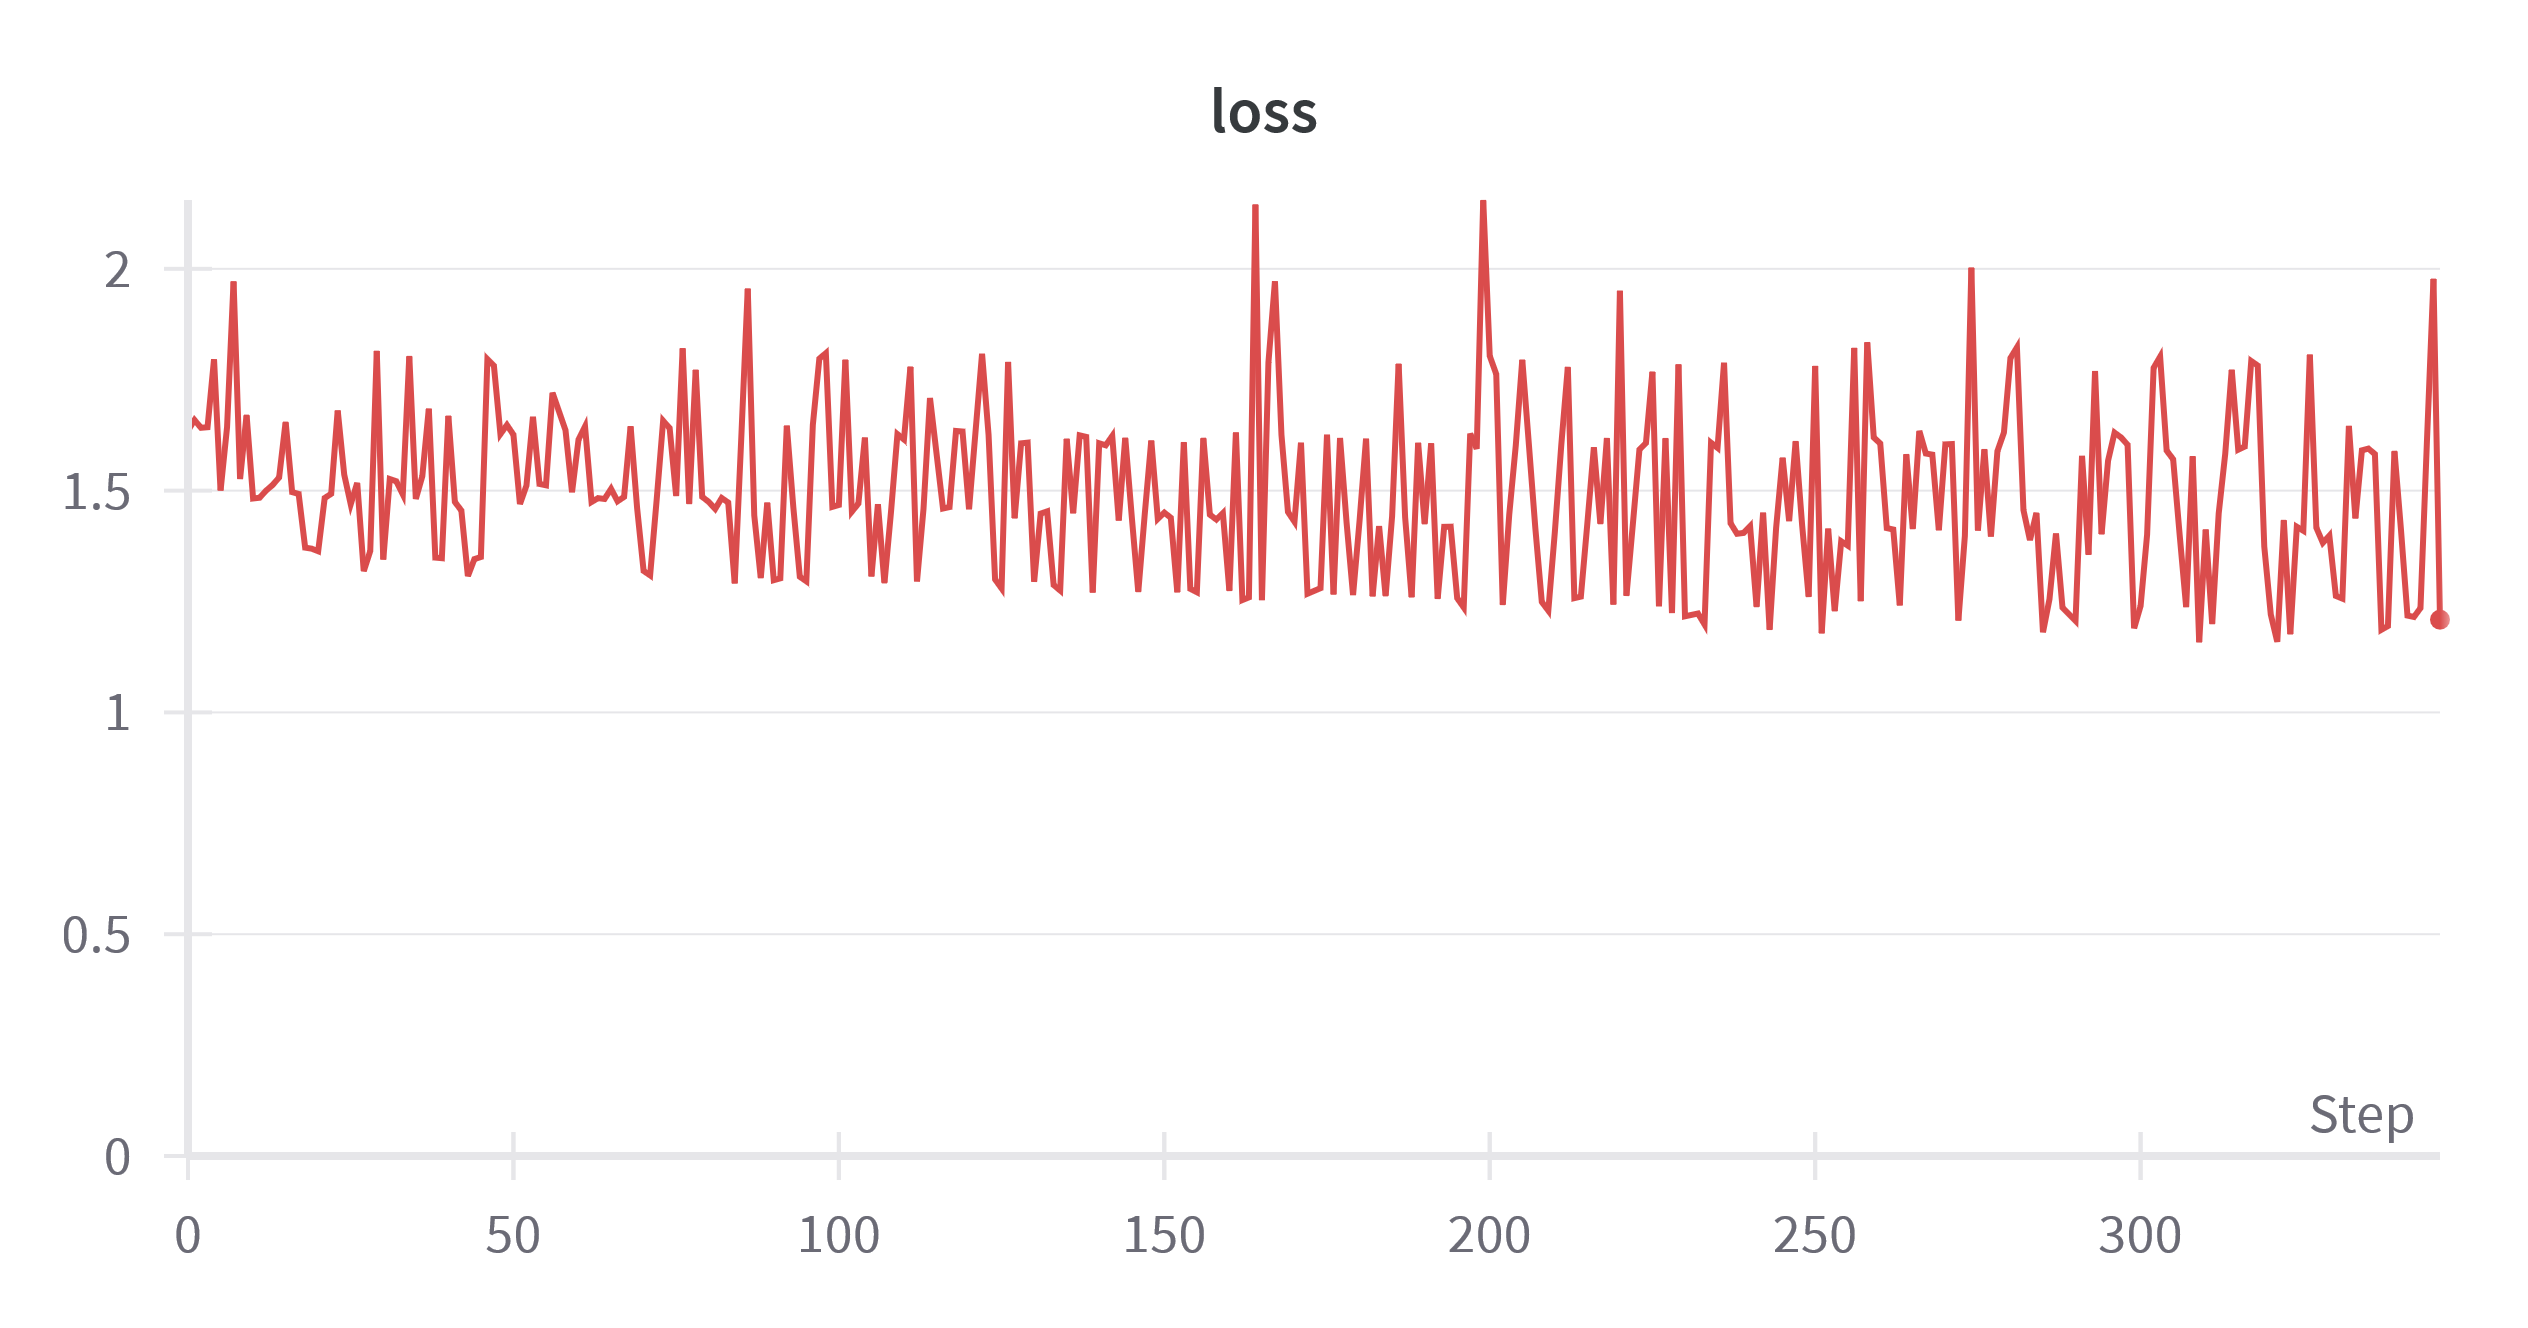
\includegraphics[width=1\textwidth]{figures/Figure8.png}
    \caption{Loss Graph on train set using original GoogLeNet with a 5 channel input for the first layer}
    \label{fig:fig8}
\end{figure}

Evidently, the loss is not ideal. It does not appear to reduce its value after each step. This image from Figure \ref{fig:fig8}) consists of the loss of the model calculated for 6 epochs, and the predictions made on the test data were not ideal either, because they seemed to only predict normal or actionable types, disregarding the latter ones entirely. Figure \ref{fig:fig9} shows us how the confusion matrix looked after the first epochs and after the sixth one.

\begin{figure}[!ht]
    \subfigure[After epoch 1]{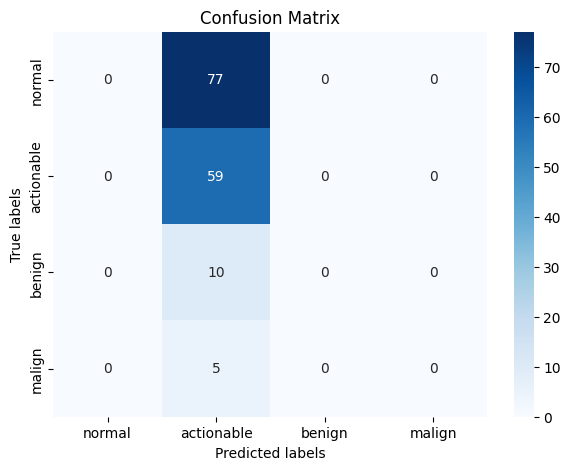
\includegraphics[width=0.45\linewidth]{figures/Figure9.png}}
    \subfigure[After epoch 6]{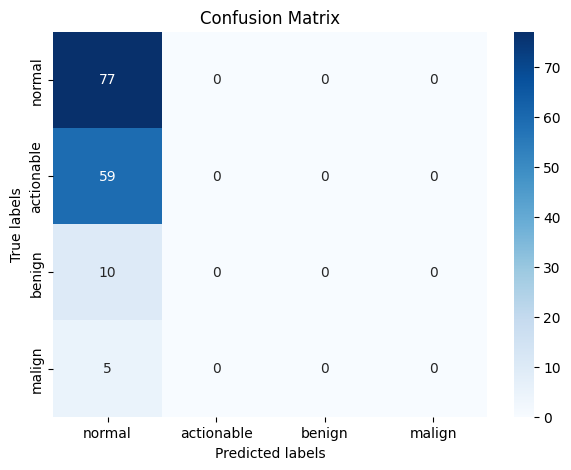
\includegraphics[width=0.45\linewidth]{figures/Figure10.png}}
    \caption{Confusion matrices for the test set ran on an original GoogLeNet architecture with a 5 channel input for the first layer}
    \label{fig:fig9}
\end{figure}

\subsection{Experiment 2}

The second experiment proved to be a little more fruitful. I changed the learning rate to 0.0001, the optimizer to Adam and employed learning rate decay, more exactly a step learning rate decay with a step size of 4 and a gamma of 0.1. The batch size was changed to 8, and I utilized a batch sampler class to correctly distribute the different input types into the batches in order to have a better proportion of classes. I was also under the impression that the GoogleNet architecture was maybe too deep to predict the images, so I experimented with the two auxiliary modules that GoogleNet provides. Therefore, the model for this experiment is the same one as the GoogLeNet architecture, but moving the first auxiliary model higher, as shown in figure \ref{fig:fig41}. For this experiment, I trained the model using the first auxiliary while also modifying the forward-pass function to only include two inception layers.

\begin{figure}
    \centering
    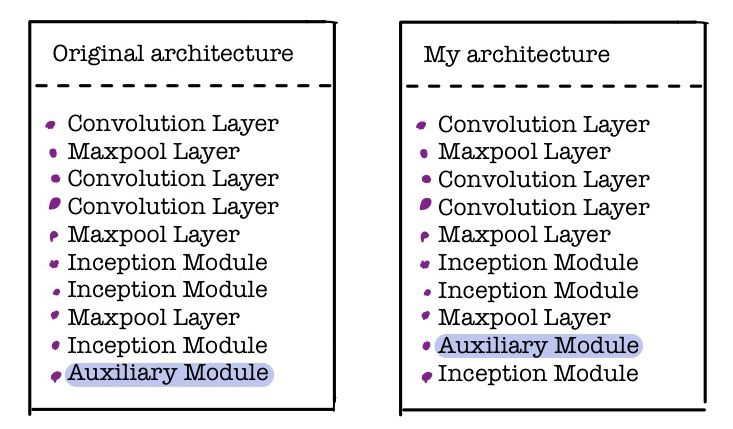
\includegraphics[width=0.5\linewidth]{figures/Figure53.png}
    \caption{Difference between the architecture of the original GoogLeNet and the configuration for the second experiment}
    \label{fig:fig41}
\end{figure}

Additionally, I changed the weights for the benign and malign classes in the loss function, substituting 4 for 6 for both of them. Figure \ref{fig:fig10} shows how the loss graph looked after training eight epochs and another 21 batches in the ninth epoch.

\begin{figure}[!ht]
    \centering
    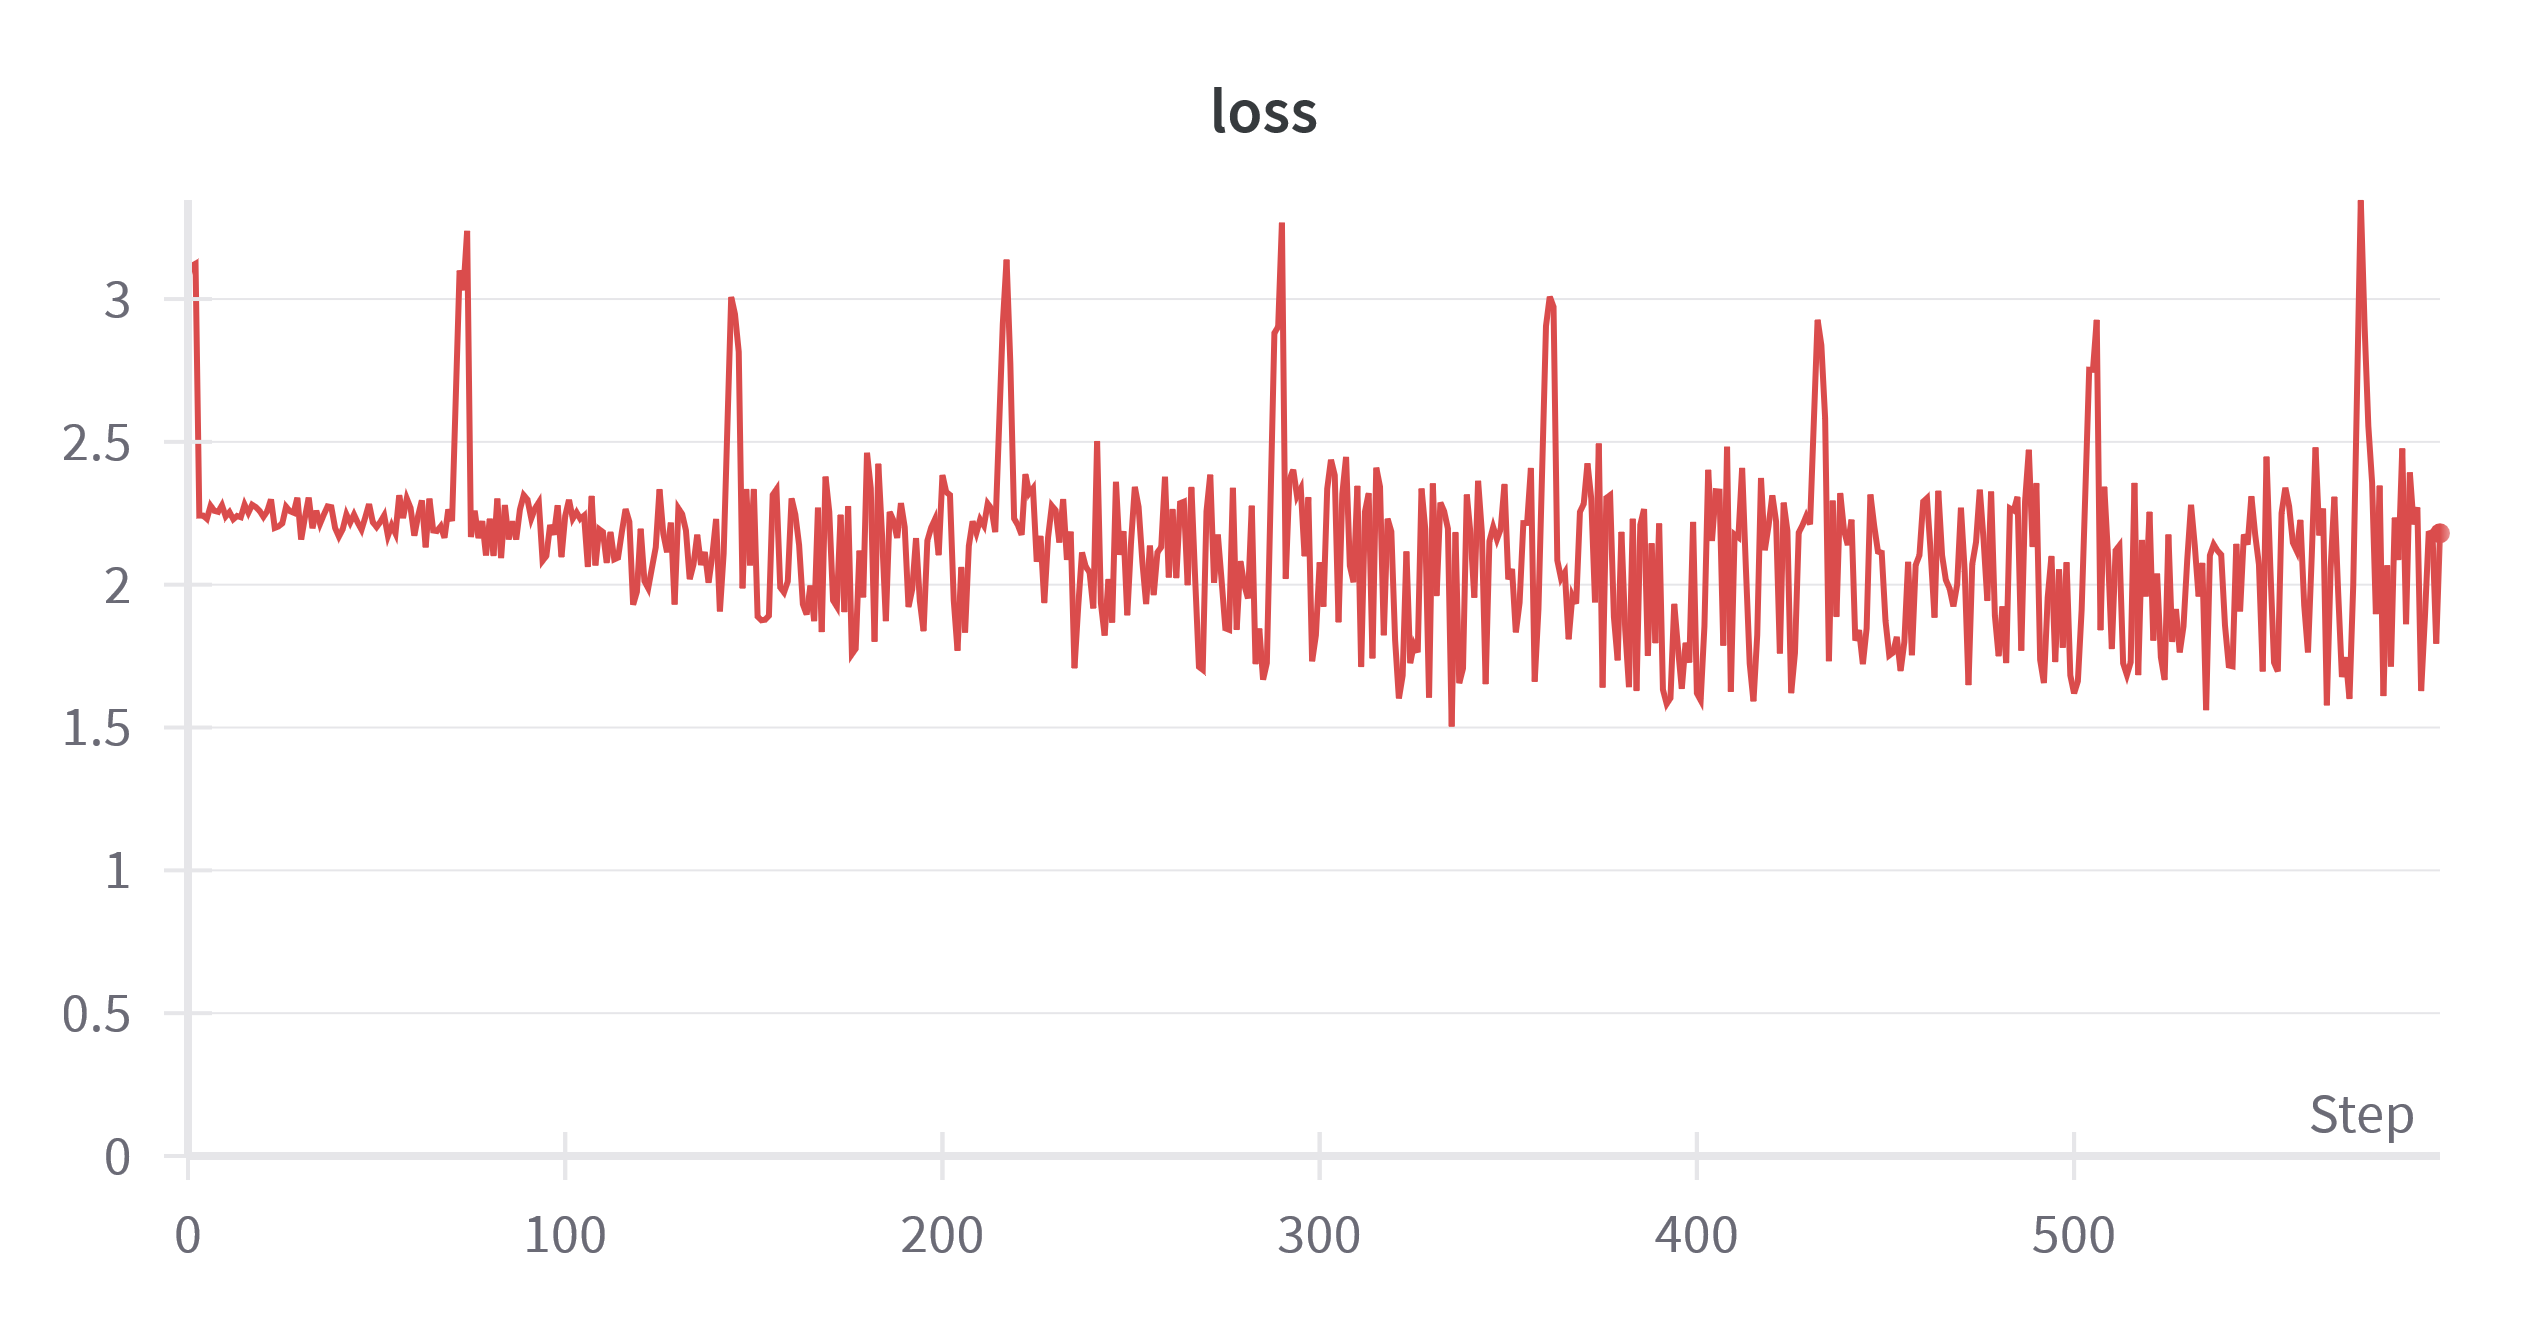
\includegraphics[width=1\textwidth]{figures/Figure11.png}
    \caption{Loss Graph on train set using the first auxiliary module from the modified GoogLeNet architecture with a 5 channel input for the first layer}
    \label{fig:fig10}
\end{figure}

This time around, the model started to also predict images of class malign, but only after the first epoch. Curiously, it did not predict any images to be of type benign, even after eight epochs. Figure \ref{fig:fig11} shows how the predictions looked after the first and eighth epochs.

\begin{figure}[!ht]
    \subfigure[After epoch 1]{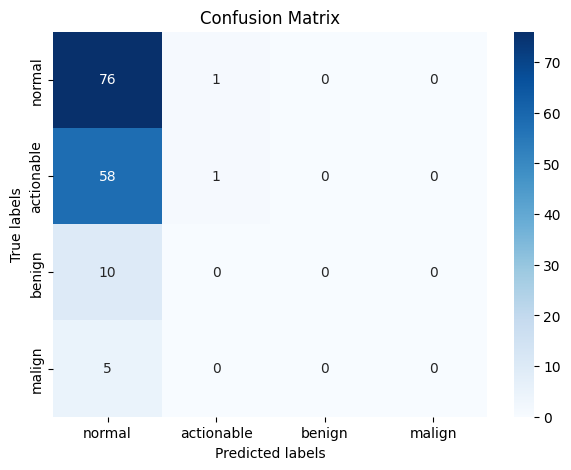
\includegraphics[width=0.45\linewidth]{figures/Figure12.png}}
    \subfigure[After epoch 2]{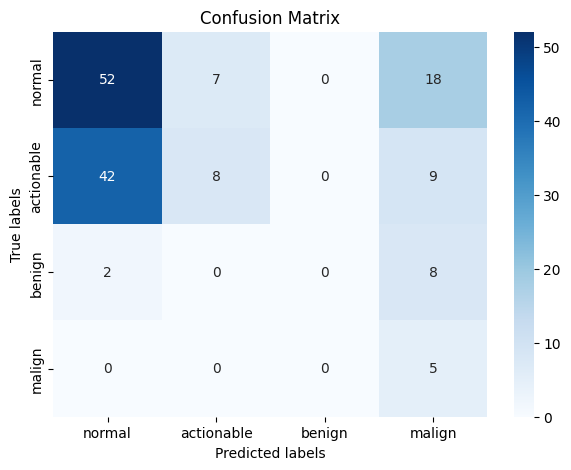
\includegraphics[width=0.45\linewidth]{figures/Figure13.png}}
    \caption{Confusion matrices for the test set ran on the first auxiliary module from the modified GoogLeNet architecture with a 5 channel input for the first layer}
    \label{fig:fig11}
\end{figure}

\subsection{Experiment 3}

The only difference between this second experiment and the third was that the learning rate decay was changed from step to exponential with a gamma of 0.8. This means that the configuration for the forward-pass method is also the same, as shown in figure \ref{fig:fig41} .Figure \ref{fig:fig13} depicts the difference in loss between these two experiments.

\begin{figure}[!ht]
    \centering
    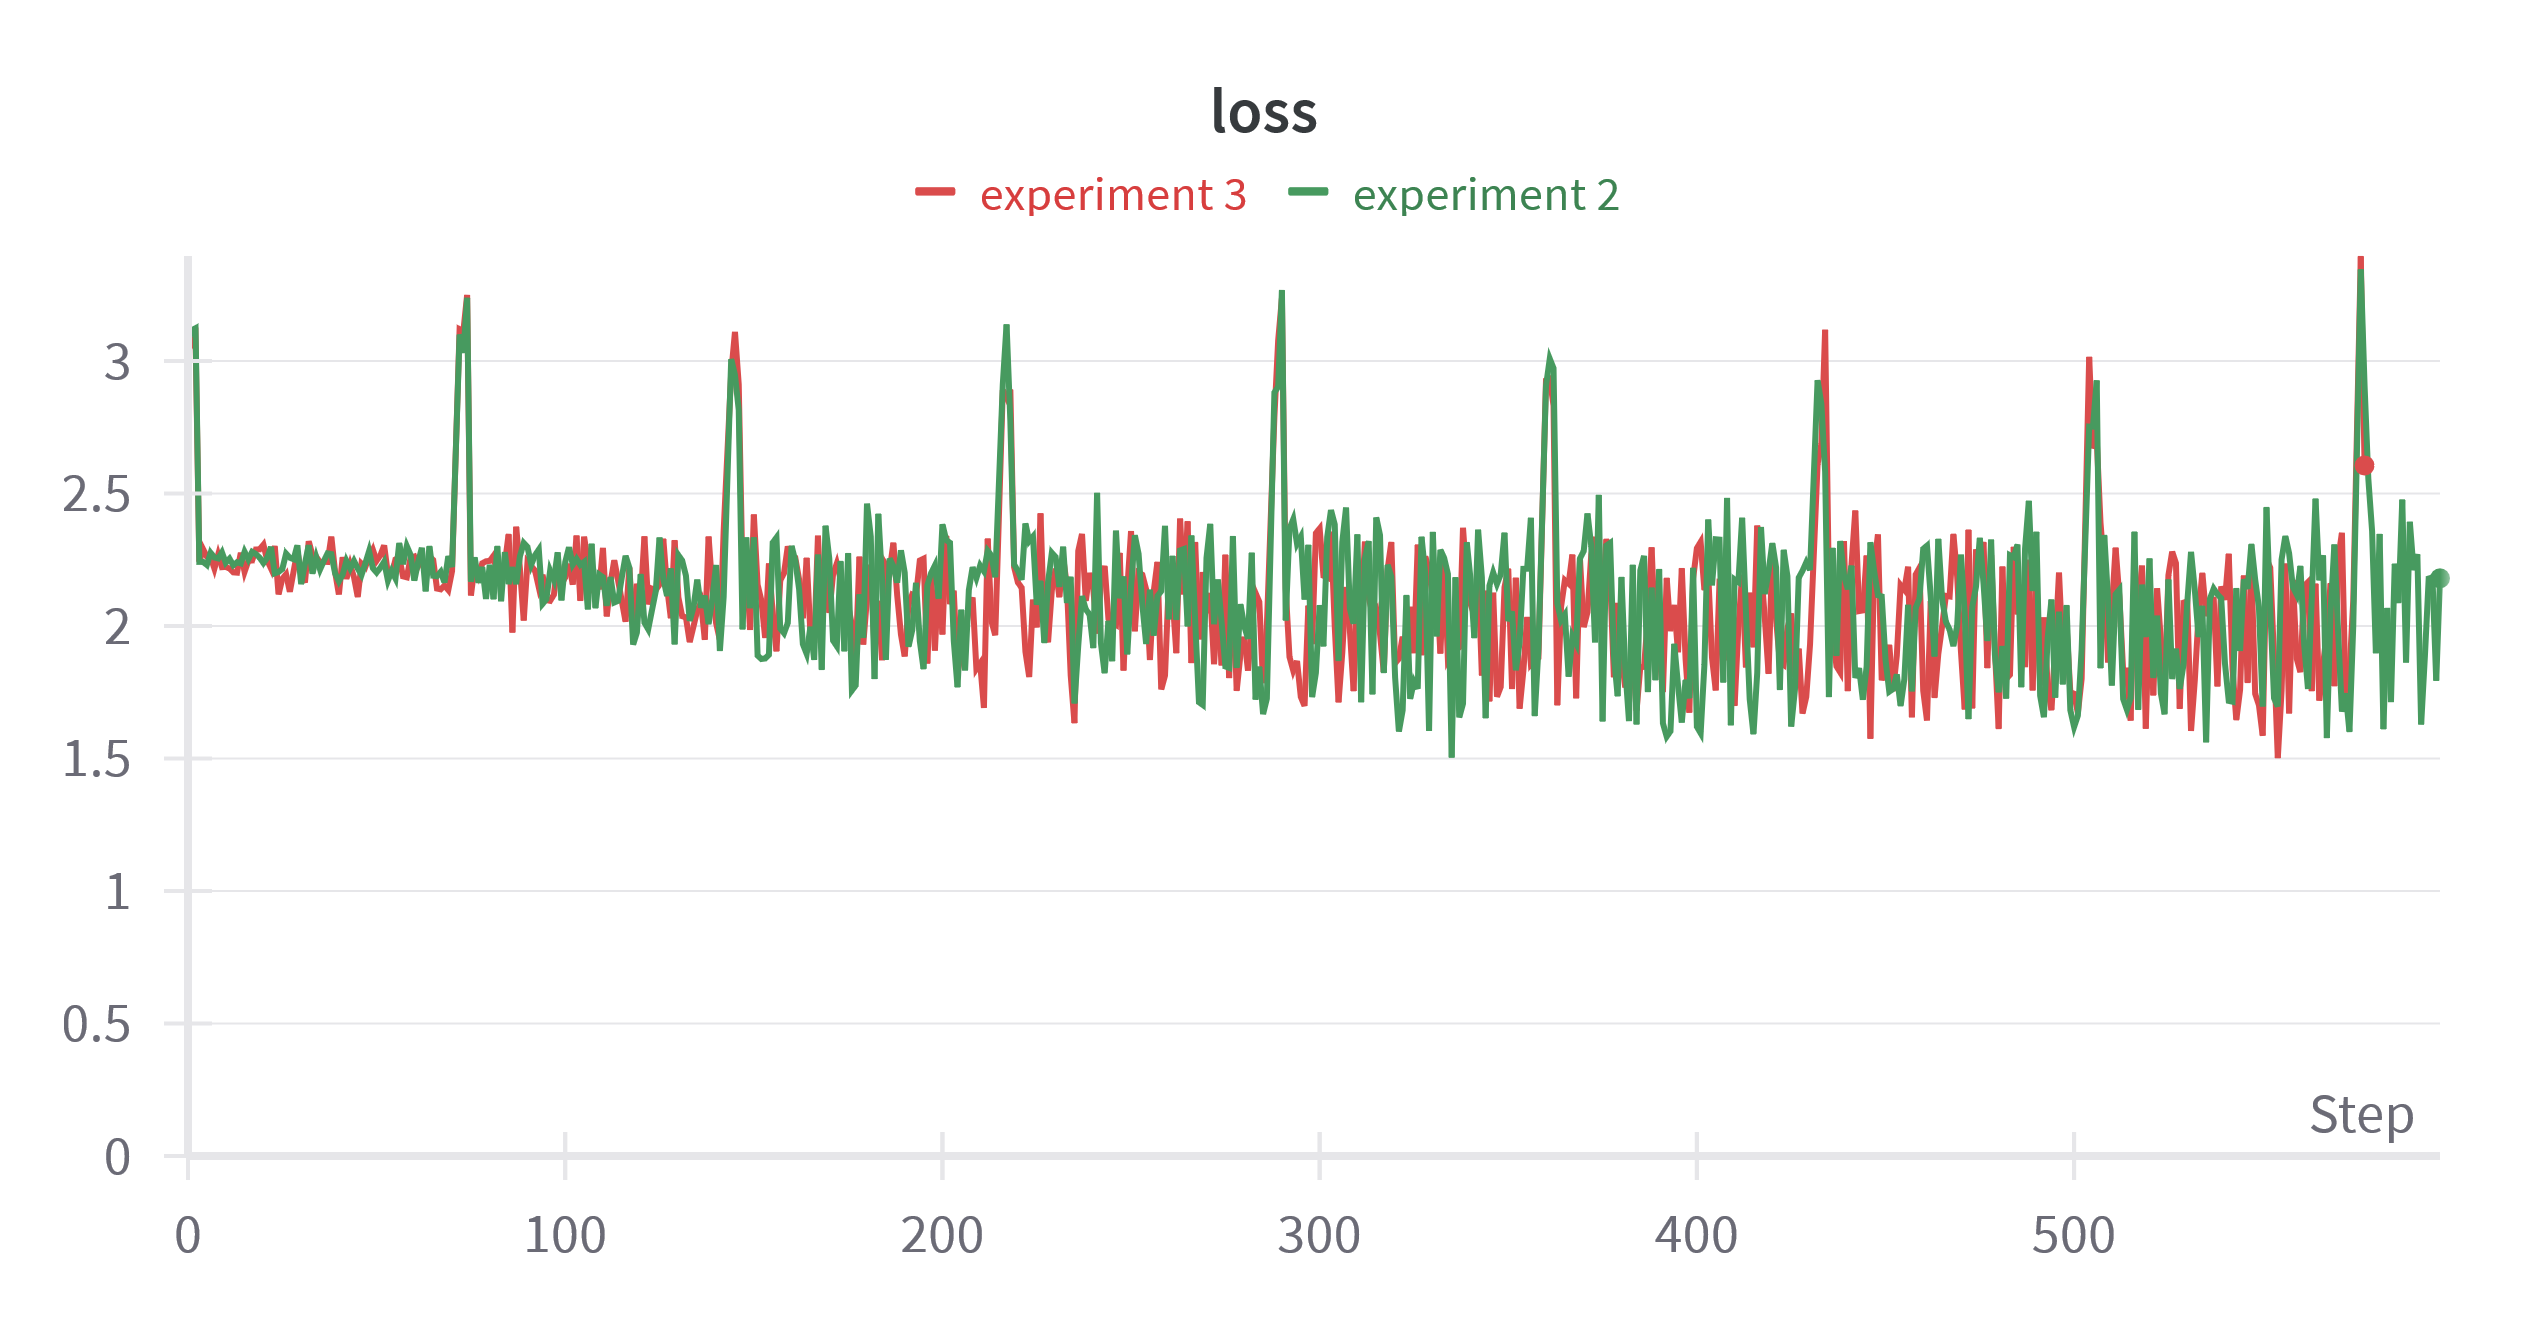
\includegraphics[width=1\textwidth]{figures/Figure14.png}
    \caption{Loss Graph on train set using the first auxiliary module from the modified GoogLeNet architecture with a 5 channel input for the first layer}
    \label{fig:fig13}
\end{figure}

The predictions for the third experiment were very similar to the ones from the second experiment, meaning the model would predict only three classes out of all four of them.

The spikes in Figure \ref{fig:fig10} represent the batches that had more input of classes benign and malign because the number of classes did not allow for equally proportionate batches of eight. I thought that the randomness in which these batches appeared could negatively impact the overall accuracy of the model, so in further experiments, I changed this way of thinking and made these batches appear first. Figure \ref{fig:fig13} shows how the experiment turned out, so not much was changed, and the predictions overall on the test data were not different.

\subsection{Experiment 4}

For the next experiment, I stopped considering this a problem of 4-label detection but rather a 2-label detection. Therefore, I grouped the actionable, benign and malign types into one and trained the model using this group and the normal ones. I kept everything else in terms of configuration, including the structure of the architecture, from the third to the fourth experiment, except for batch size, which I changed to 64. Figure \ref{fig:fig16} shows how the loss looked after training three epochs on the training data, and Figure \ref{fig:fig17} shows how the confusion matrix looked after those three epochs on the testing data. Table \ref{tab:tab2} shows the distribution between the classes in the train set and test set.

\begin{table}[ht!]
\centering
\begin{tabular}{|c|c|c|c|}
    \hline
    & Train set & Test set \\ \hline
    Size & 568 & 151 \\ \hline
    Normal & 273 & 77\\ \hline
    Cancer & 295 & 74\\ \hline
    \end{tabular}
    \caption{Experiment 4 --- data distribution}
    \label{tab:tab2}
\end{table}

\begin{figure}[!ht]
    \centering
    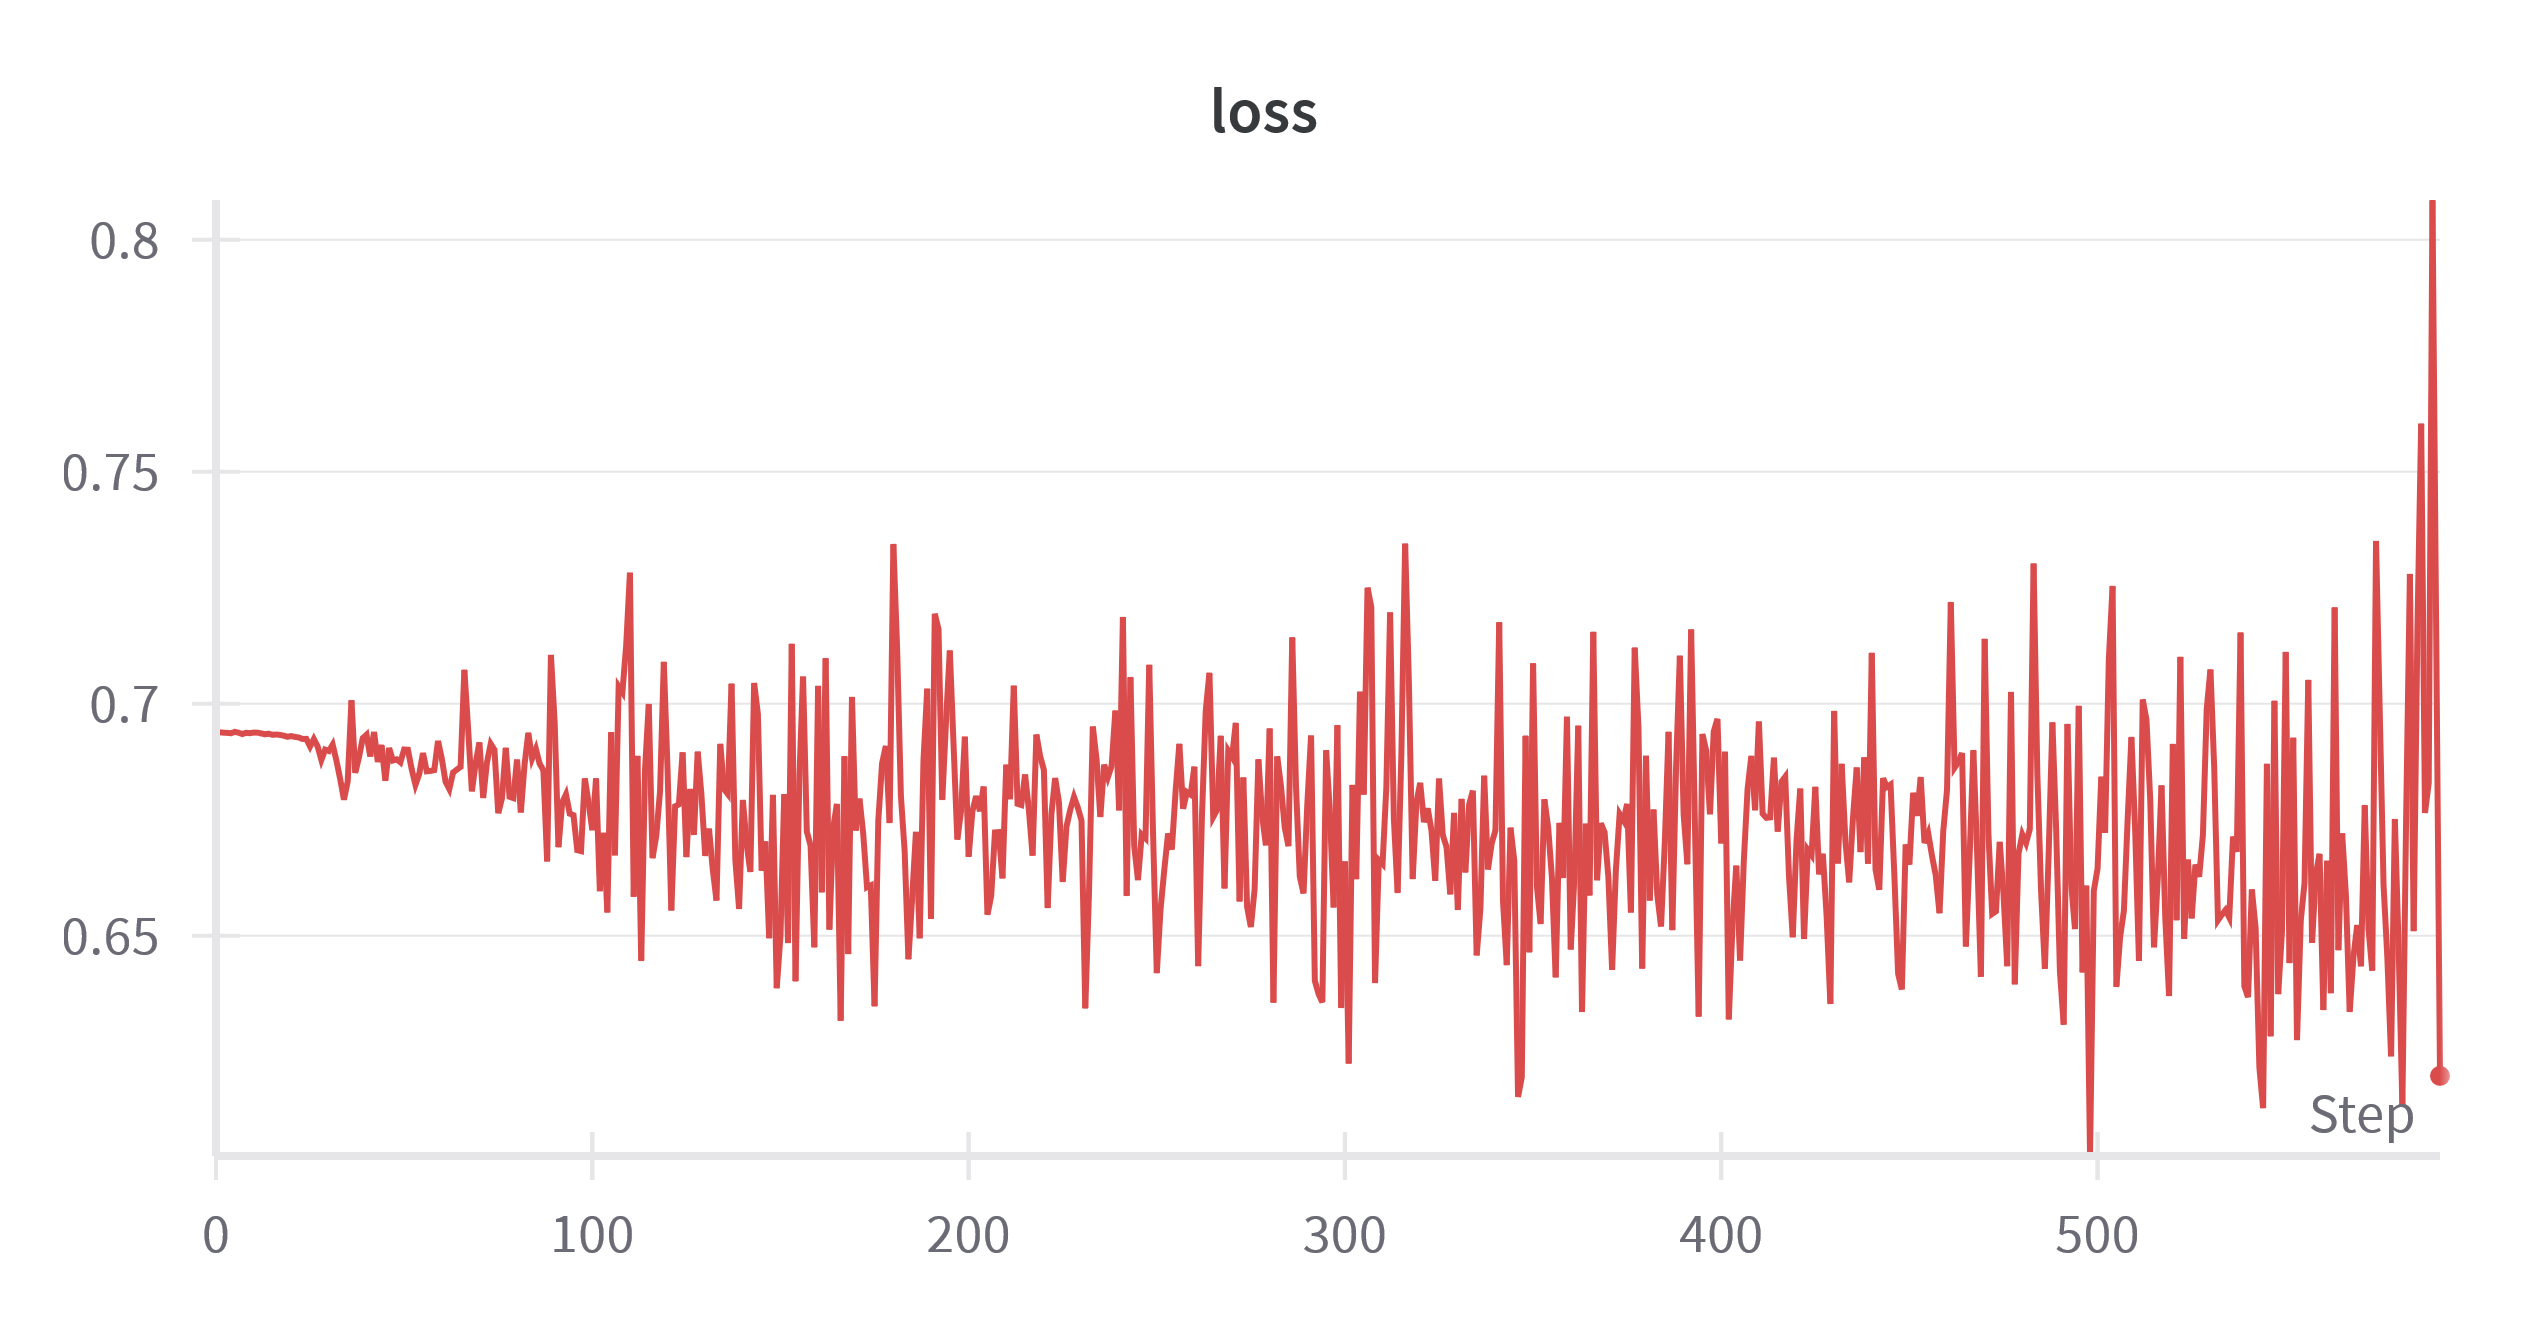
\includegraphics[width=0.75\linewidth]{figures/Figure17.png}
    \caption{Loss Graph on train set using the first auxiliary module from the modified GoogLeNet architecture with a 5 channel input for the first layer}
    \label{fig:fig16}
\end{figure}

\begin{figure}[ht]
    \centering
    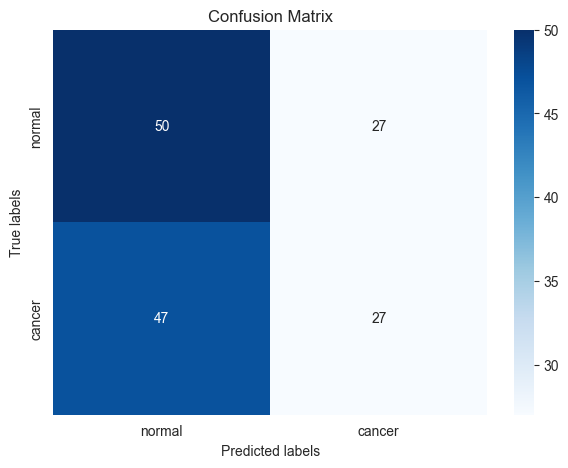
\includegraphics[width=0.45\linewidth]{figures/Figure18.png}
    \caption{Confusion matrices for test set ran for three epochs on the first auxiliary module from the modified GoogLeNet architecture with a 5 channel input for the first layer}
    \label{fig:fig17}
\end{figure}

\subsection{Experiment 5}

I resized the images to be 300$\times$300, and instead of adding the slices as channels of the same image, I added the slices as individual inputs. In doing so, I transformed a 568-length dataset into a 2,840-length one and used a batch size of 64.

Upon figuring out the number of learnable parameters, which was around 3 million, I wanted to increase the length of the dataset even more. With this purpose in mind, I considered 22 slices of each input, and adding each of them individually resulted in a 12,496-length dataset. This also meant that I stopped providing the model with 3D images, instead adding each input as an image of size 3$\times$W$\times$H.

\begin{table}[ht!]
\centering
\begin{tabular}{|c|c|c|c|}
    \hline
    & Train set & Test set \\ \hline
    Size & 12496 & 3322 \\ \hline
    Normal & 6006 & 1694\\ \hline
    Cancer & 6490 & 1628\\ \hline
    \end{tabular}
    \caption{Experiment 5 distribution}
    \label{tab:tab3}
\end{table}

Additionally, I wanted to compare the loss of the two auxiliary models that GoogLeNet has to offer with the main output that it returns. In doing so, I returned to the initial implementation of the forward-pass method. However, I made a mistake in that I forgot that the original implementation doesn't include either activation function on the last layer, instead adding one only for the main output, not for the two auxiliary modules. Curiously, these two modules proved to obtain the lowest loss of all the experiments I performed, as shown in figure \ref{fig:fig18}.

\begin{figure}[ht]
    \centering
    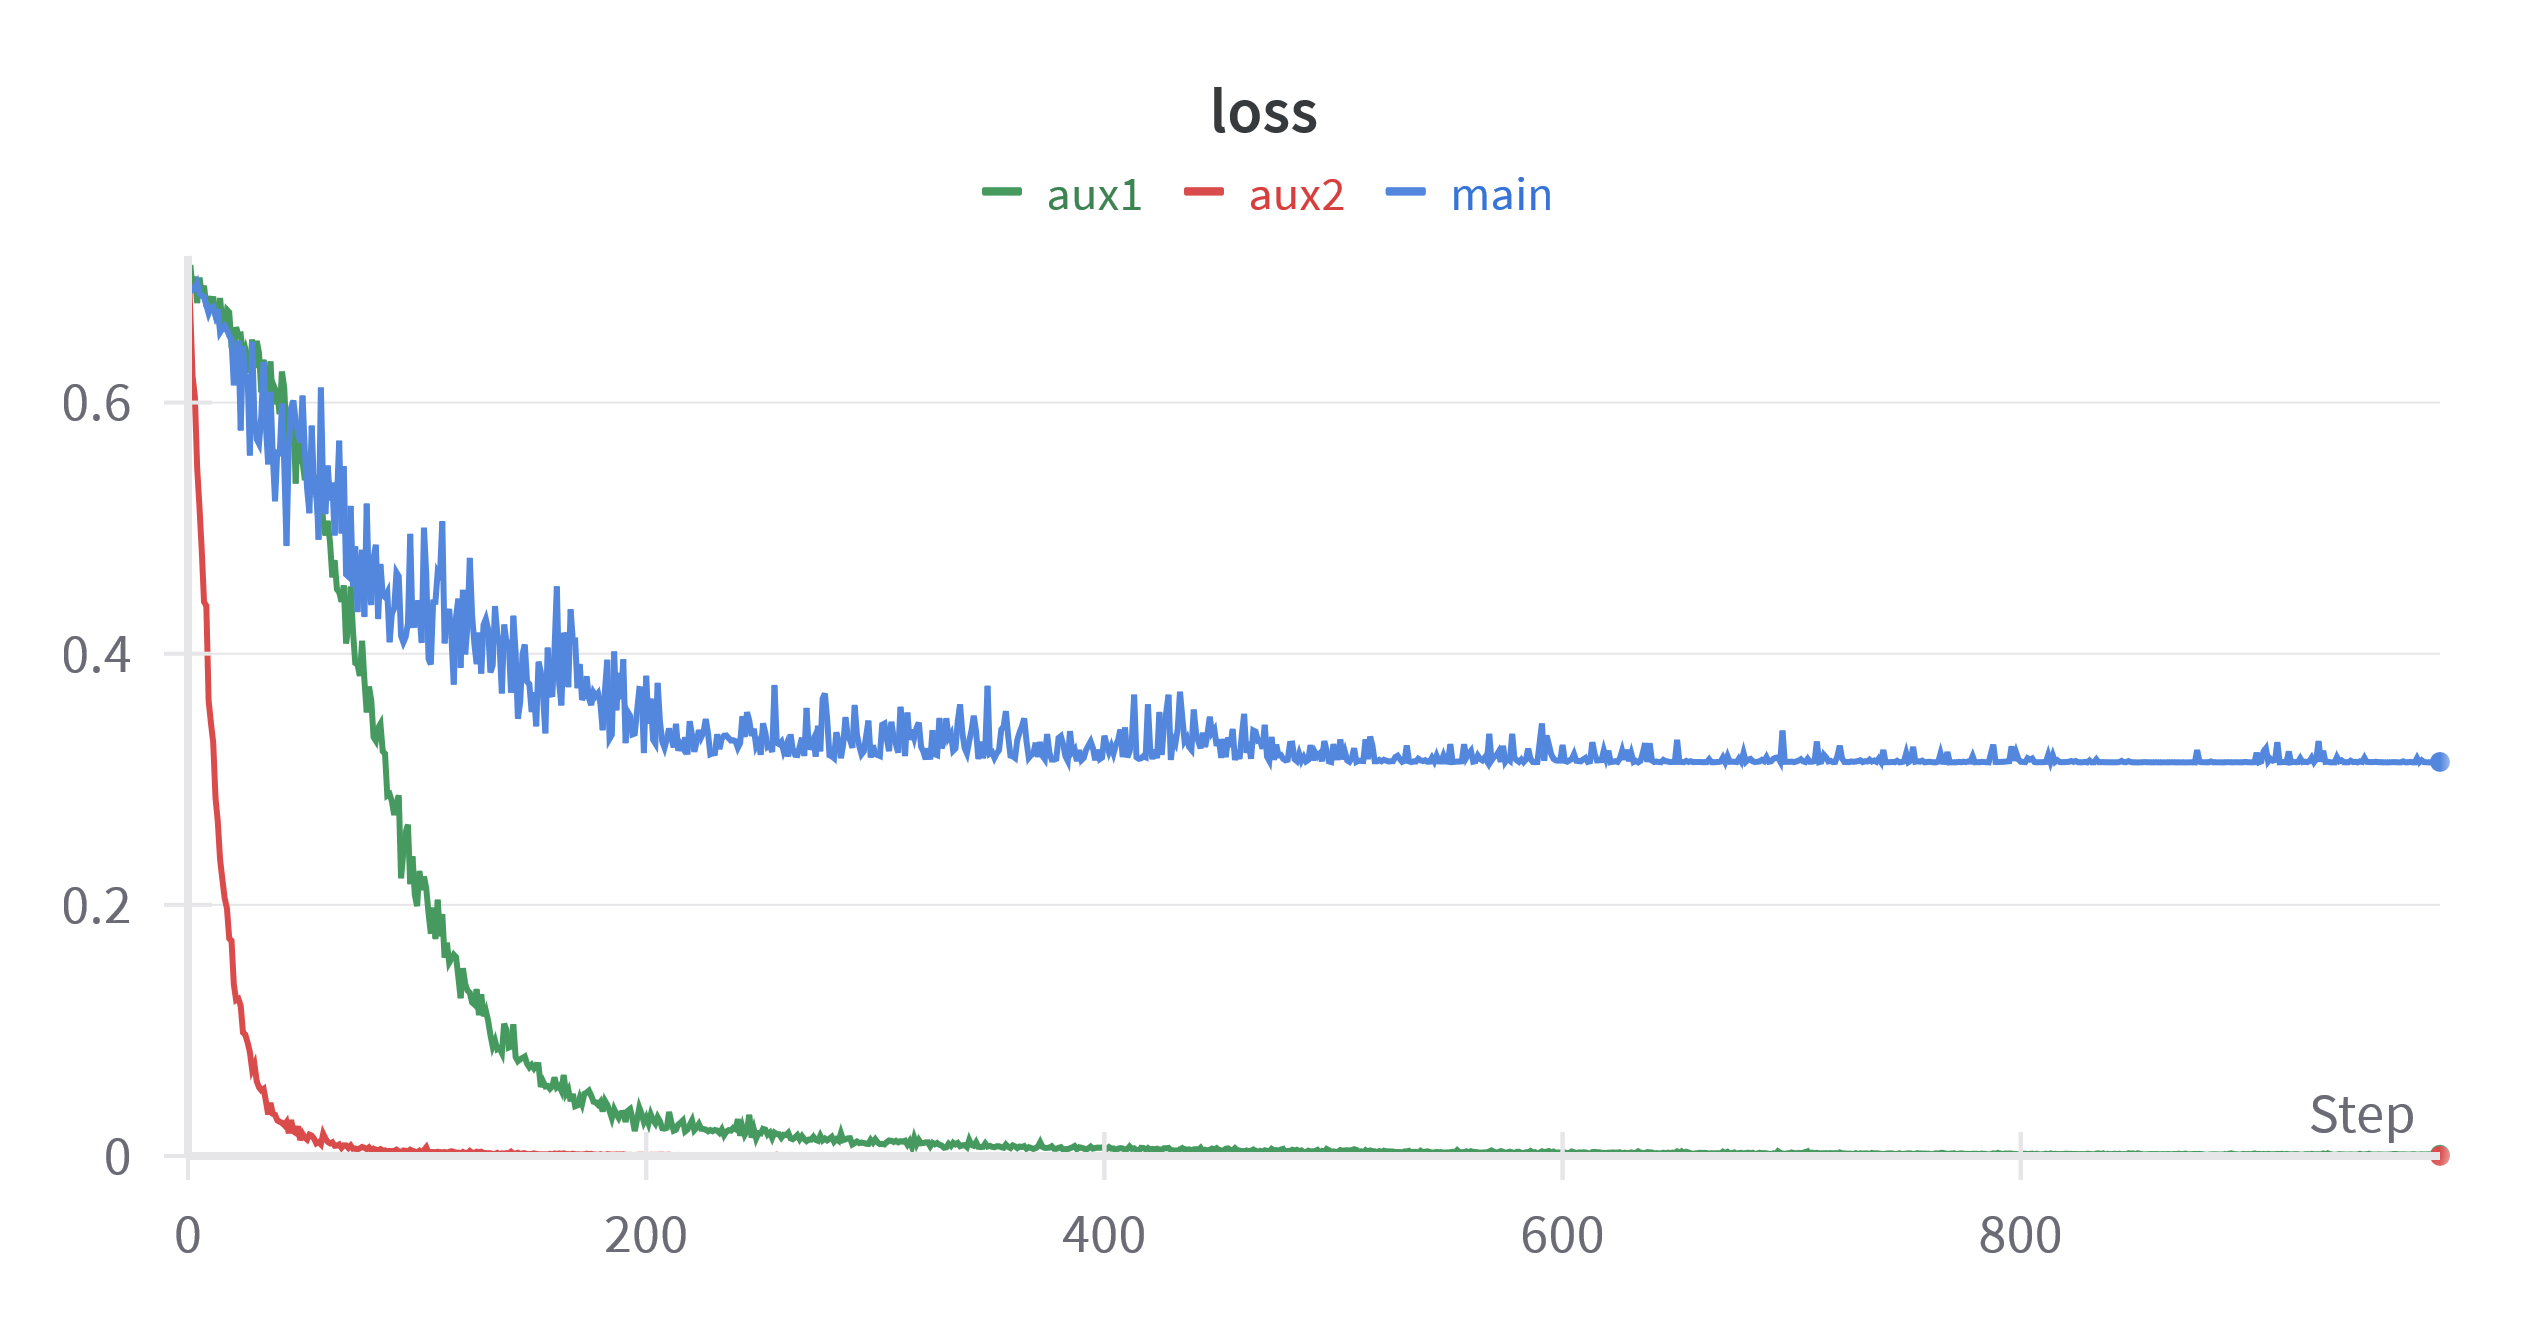
\includegraphics[width=0.75\linewidth]{figures/Figure19.png}
    \caption{Loss Graph on train set using both the auxiliary modules and the main module from the original GoogLeNet architecture with a 3 channel input for the first layer}
    \label{fig:fig18}
\end{figure}

Even with all these experiments and improvements, the best accuracy I managed to obtain was 0.5409, obtained using the main module from the fifth experiment configuration, after five epochs, as shown in figure \ref{fig:fig32}.

\begin{figure}[H]
    \centering
    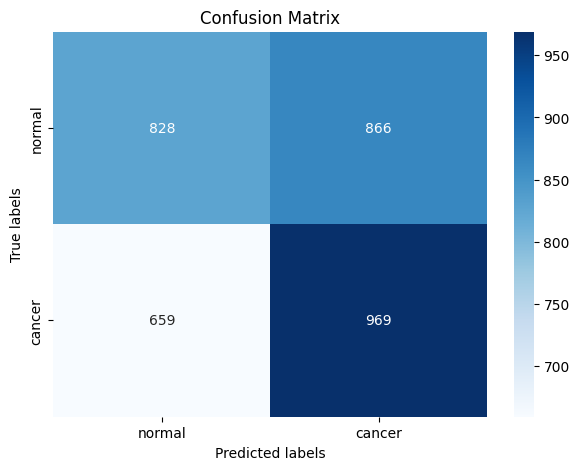
\includegraphics[width=0.5\linewidth]{figures/Figure39.png}
    \caption{Confusion matrices for test set ran for 5 epochs on the main module from the pre-trained GoogLeNet architecture with a 3 channel input for the first layer}
    \label{fig:fig32}
\end{figure}

\subsection{Experiment 6}

Towards the end of the process of training the classification model, I decided to use already GoogLeNet trained weights from the Torchvision library. The nature of these pre-trained weights does not allow direct access to the auxiliary modules, though the forward-pass method could have been overwritten. I, however, chose not to do this, instead opting to only examine the output from the main module.

These weights had been trained on images from ImageNet. Therefore, the experiments to come represent a fine-tunning of the pre-trained model acquired. The model was trained on the ImageNet Large Scale Visual Recognition Challenge (ILSVRC) contest in 2014~\cite{carte12}, which contains 456567 images for training~\cite{link16}. I also resized the images again and made them 512x512 in order to also fit the detection model. Figure \ref{fig:fig19} shows the loss graph after training the model for 5 epochs, while figure \ref{fig:fig20} shows the confusion matrix at the end of those epochs.

\begin{figure}[!ht]
    \centering
    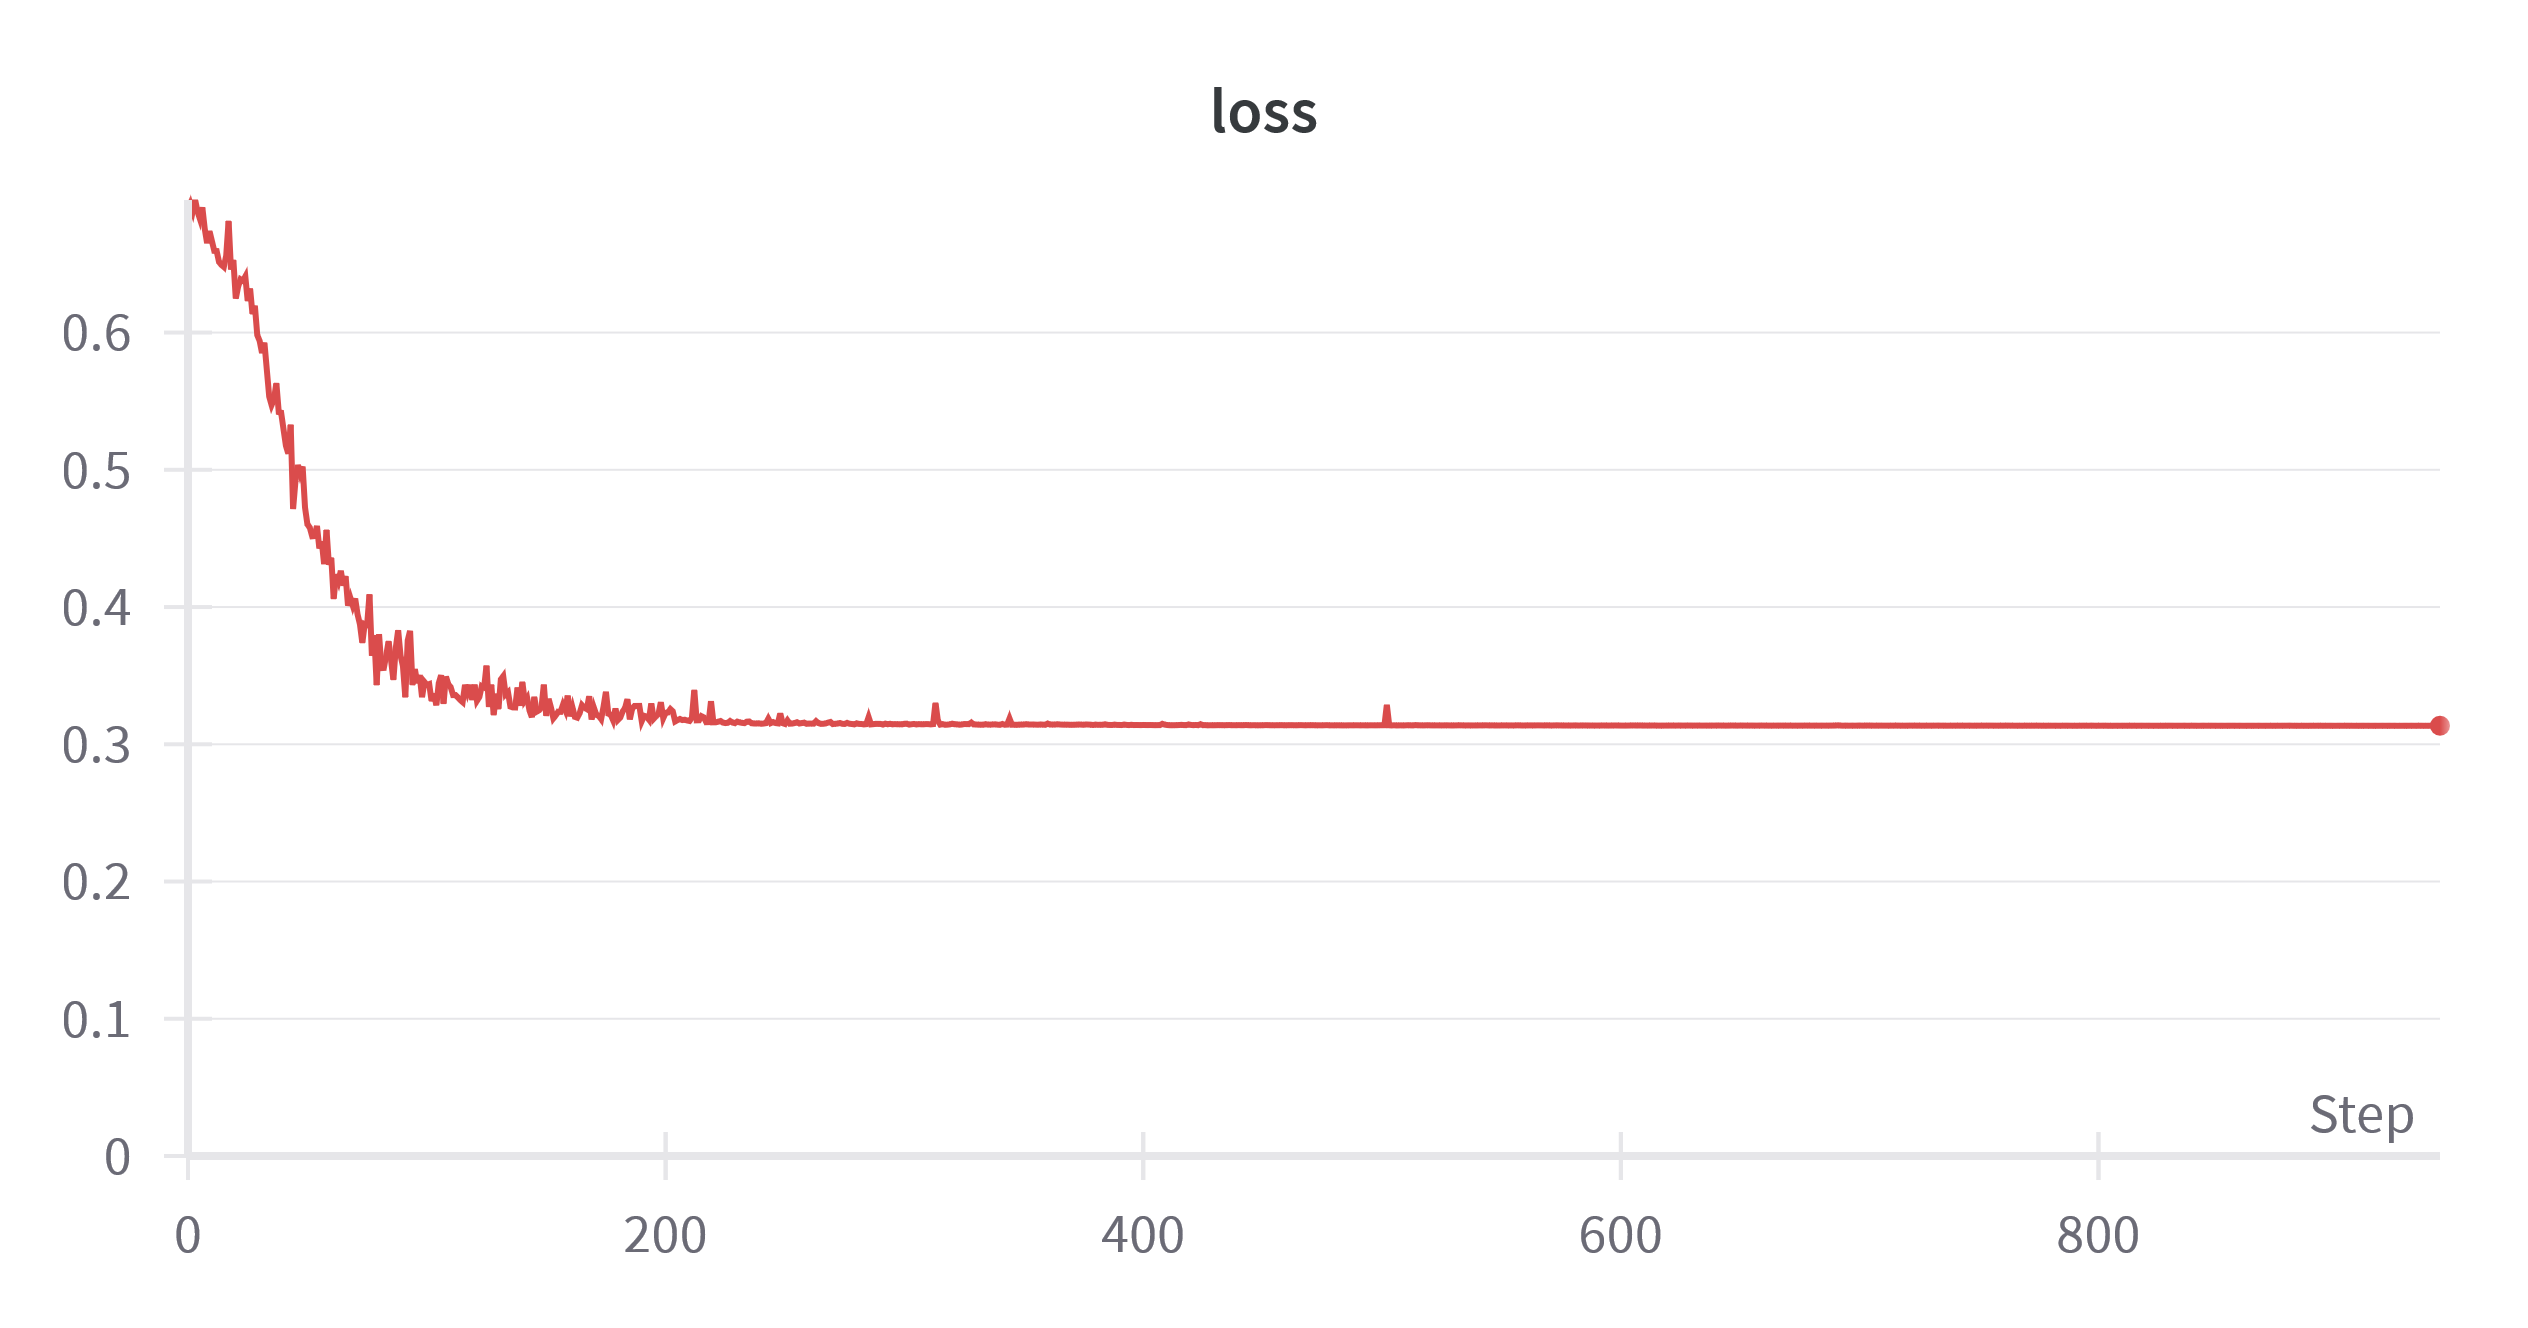
\includegraphics[width=1\linewidth]{figures/Figure20.png}
    \caption{Loss Graph on train set using the main module from the pre-trained GoogLeNet architecture with a 3 channel input for the first layer}
    \label{fig:fig19}
\end{figure}

\begin{figure}[!ht]
    \centering
    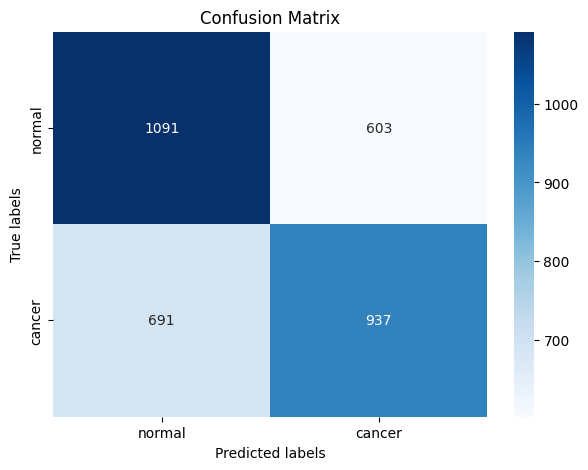
\includegraphics[width=0.5\linewidth]{figures/Figure21.png}
    \caption{Confusion matrices for test set ran for 5 epochs on the main module from the pre-trained GoogLeNet architecture with a 3 channel input for the first layer}
    \label{fig:fig20}
\end{figure}

I also experimented with different batch sizes for the pre-trained model on ImageNet weights.

Therefore, I trained the model with the same configuration as the previous run, except I modified the size of the batches from 64 to 128. Figure \ref{fig:fig21} shows the comparison in loss between these two experiments. This second model I also trained for 5 epochs; however, the difference in steps in the graph comes from increasing the number of inputs in each batch, which means fewer batches over the dataset and overall fewer steps.

\begin{figure}[H]
    \centering
    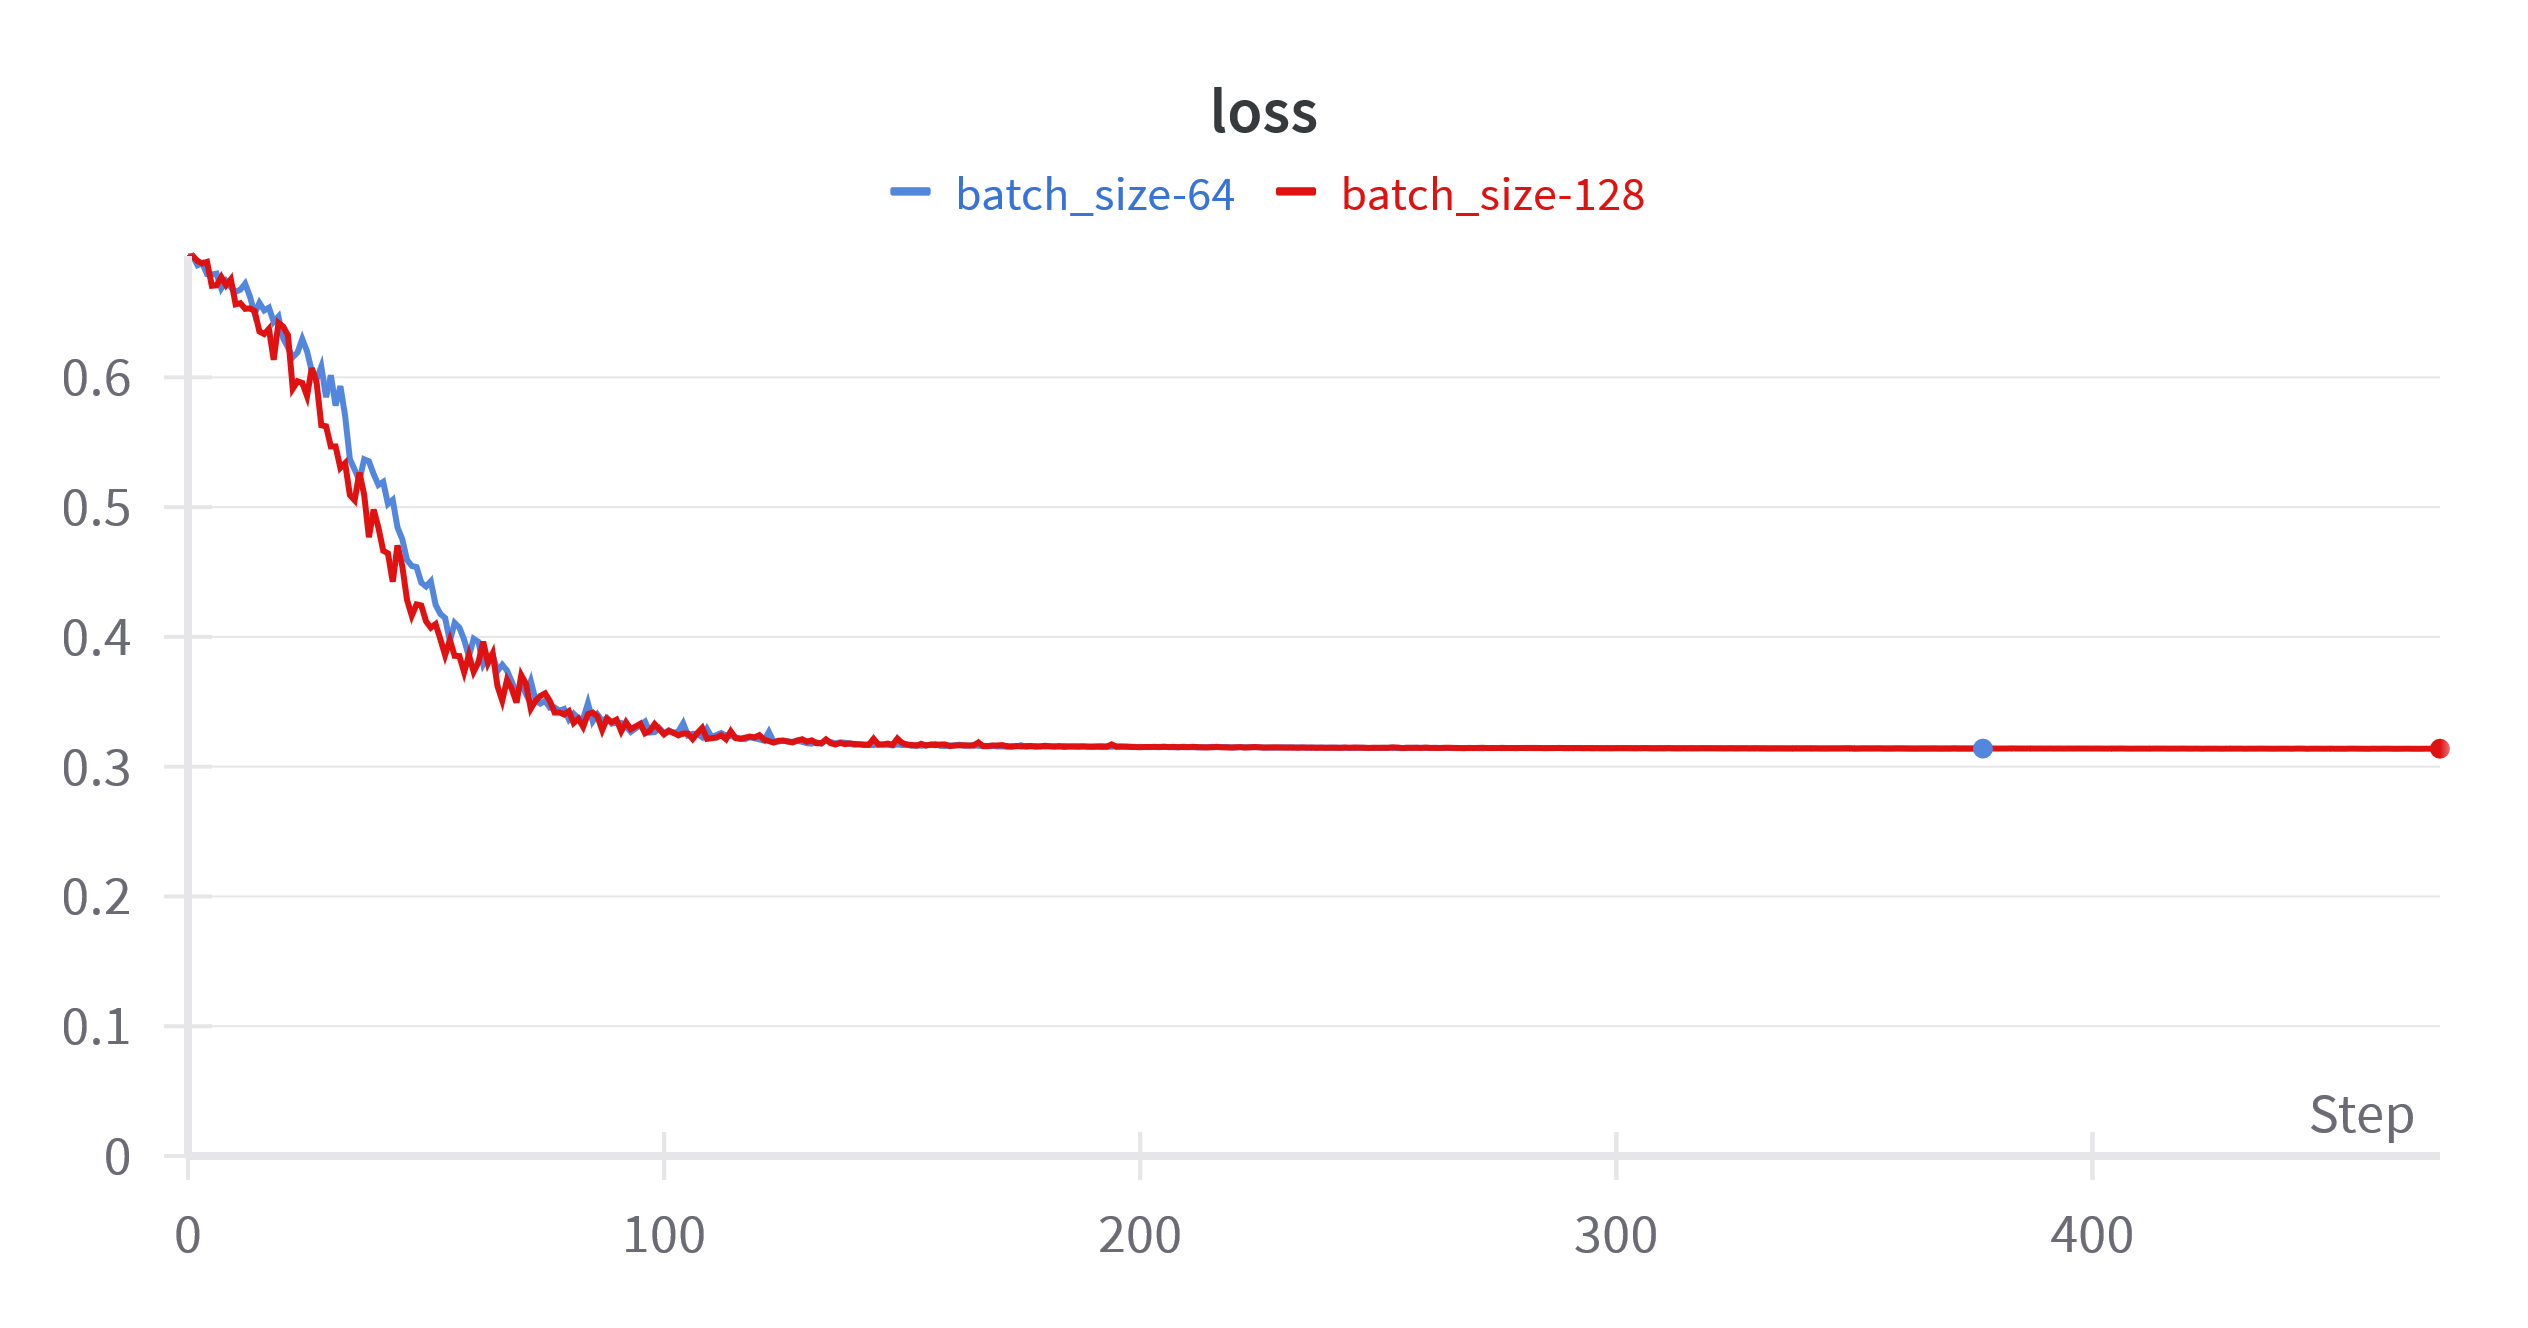
\includegraphics[width=0.75\linewidth]{figures/Figure22.png}
    \caption{Comparison between the losses obtained on the train set using the main module from the pre-trained GoogLeNet architecture with a 3 channel input for the first layer, and different sized batches}
    \label{fig:fig21}
\end{figure}

\begin{figure}[!ht]
    \centering
    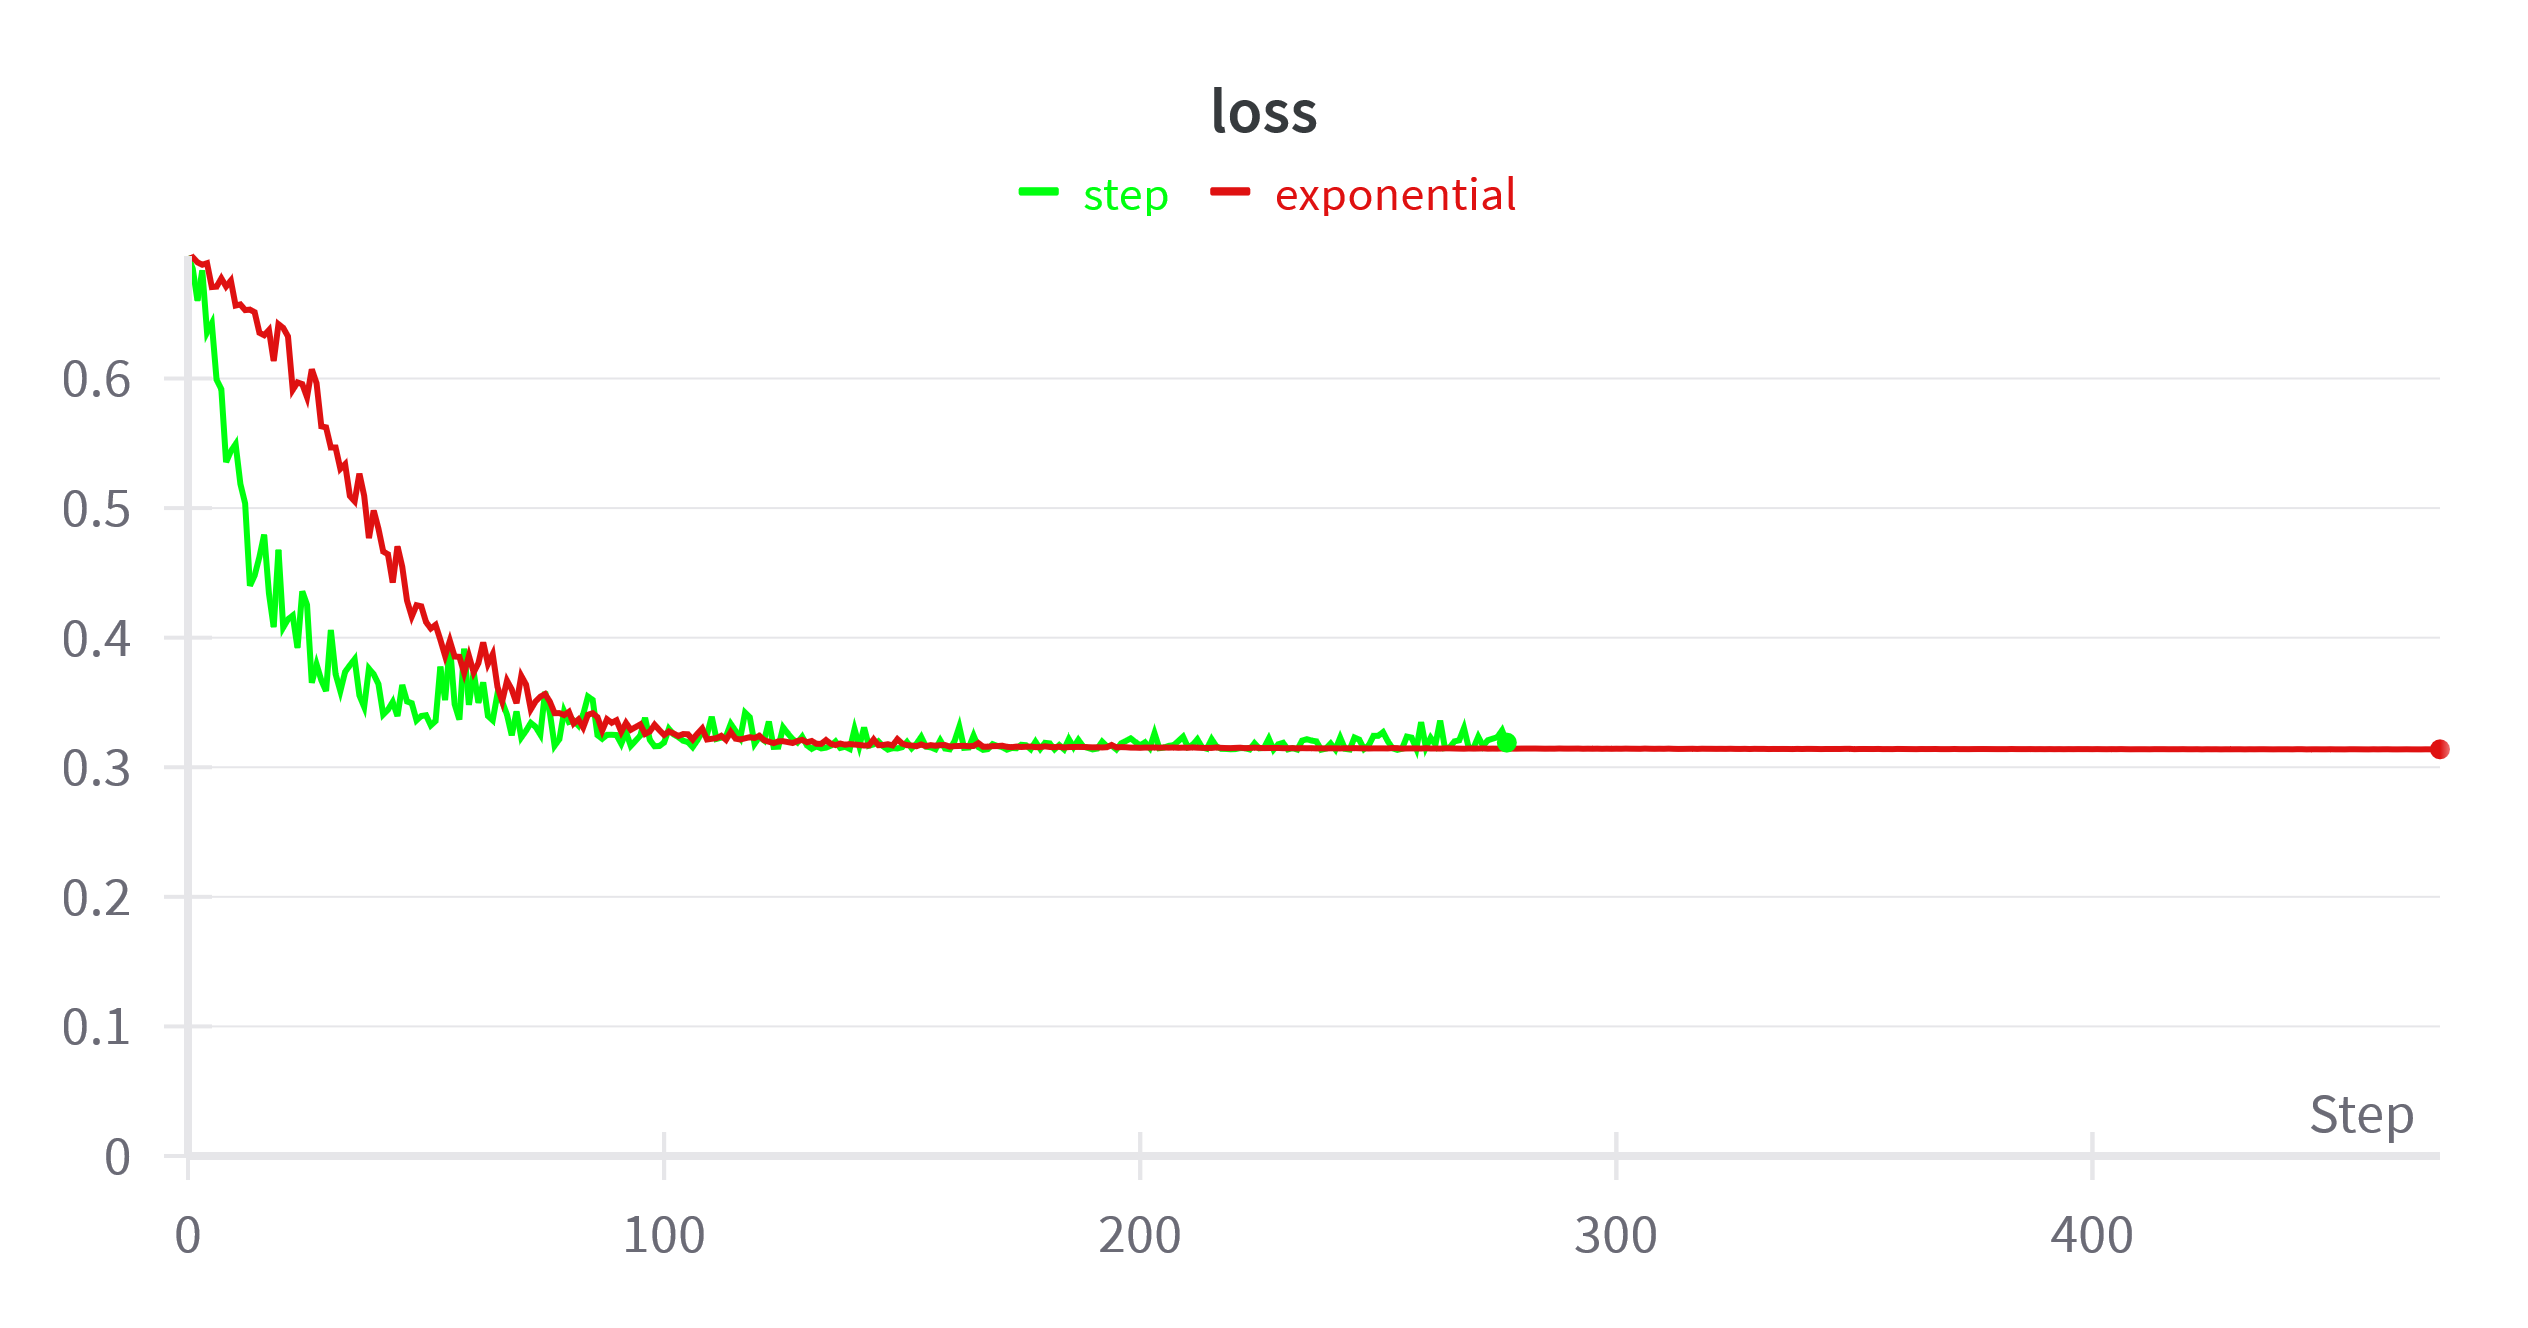
\includegraphics[width=1\linewidth]{figures/Figure24.png}
    \caption{Comparison between the losses obtained on the train set using the main module from the pre-trained GoogLeNet architecture with a 3 channel input for the first layer, and different types of learning rate decay}
    \label{fig:fig22}
\end{figure}

\begin{figure}[H]
    \centering
    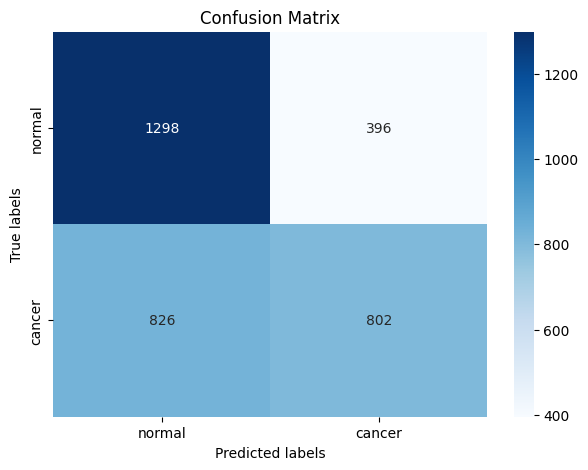
\includegraphics[width=0.5\linewidth]{figures/Figure37.png}
    \caption{Confusion matrices for the test set ran for 3 epochs on the main module from the pre-trained GoogLeNet architecture with a 3 channel input for the first layer}
    \label{fig:fig31}
\end{figure}

The final configuration that I came to included: batches of size 128, pre-trained weights trained with images from ImageNet, a learning rate of 0.0001, learning rate decay using the StepLR implementation with a step size of 5 and gamma of 0.1, an image size of 512, and 22 inputs of each image representing different slices from the 3D scans. The loss obtained using a learning rate of Step instead of Exponential is shown in figure \ref{fig:fig22}. Figure \ref{fig:fig31} shows how the confusion matrix looked after 3 epochs using this configuration.

Tables \ref{tab:tab4}, \ref{tab:tab5} and \ref{tab:tab6} shows the conclusions of these experiments.

\begin{table}[H]
    \centering
    \begin{tabular}{|c|c|c|c|c|c|}
     \hline
     \multirow{2}{5em}{Experiment}  & \multicolumn{5}{c|}{Hyper parameters} \\ \cline{2-6}
     & learning rate & optimizer & learning rate decay & step & gamma \\
     \hline \hline
     Exp1 & 0.001 & SGD & no &  &   \\
     \hline
     Exp2 & 0.0001 & Adam & Step & 4 & 0.1 \\
     \hline
     Exp3 & 0.0001 & Adam & Exponential & & 0.8\\
     \hline
     Exp4 & 0.0001 & Adam & Exponential & & 0.8\\
     \hline
     Exp5 & 0.0001 & Adam & Exponential & & 0.8\\
     \hline
     Exp6 & 0.0001 & Adam & Step & 5 & 0.1\\
     \hline
    \end{tabular}
    \caption{Classification models(continuation)}
    \label{tab:tab5}
\end{table}

\begin{table}[H]
    \centering
    \begin{tabular}{|c|c|c|c|c|c|}
     \hline
     \multirow{2}{5em}{Experiment}  & \multicolumn{5}{c|}{Performance}
     \\ \cline{2-6}
     & Accuracy & \multicolumn{2}{c|}{Recall} & \multicolumn{2}{c|}{Precision} 
     \\ \cline{3-6}
     \hline \hline
     \multirow{4}{5em}{Exp1} & \multirow{4}{5em}{0.5099} & normal & 1 & normal & 0.51 \\ \cline{3-6}
     & & actionable & 0 & actionable & 0 \\ \cline{3-6}
     & & benign & 0 & benign & 0 \\ \cline{3-6}
     & & malign & 0 & malign & 0 \\ \cline{3-6}
     \hline
     \multirow{4}{5em}{Exp2} & \multirow{4}{5em}{0.4304} & normal & 0.675 & normal & 0.54 \\ \cline{3-6}
     & & actionable & 0.136 & actionable & 0.53 \\ \cline{3-6}
     & & benign & 0 & benign & 0 \\ \cline{3-6}
     & & malign & 1 & malign & 0.125 \\ \cline{3-6}
     \hline
     \multirow{4}{5em}{Exp3} & \multirow{4}{5em}{0.4304} & normal & 0.675 & normal & 0.54 \\ \cline{3-6}
     & & actionable & 0.136 & actionable & 0.53 \\ \cline{3-6}
     & & benign & 0 & benign & 0 \\ \cline{3-6}
     & & malign & 1 & malign & 0.125 \\ \cline{3-6}
     \hline
     \multirow{2}{5em}{Exp4} & \multirow{2}{5em}{0.5099} & normal & 0.649 & normal & 0.515 \\ \cline{3-6}
     & & cancer & 0.365 & cancer & 0.50 \\ \cline{3-6}
     \hline
     \multirow{2}{5em}{Exp5} & \multirow{2}{5em}{0.5409} & normal & 0.489 & normal & 0.557 \\ \cline{3-6}
     & & cancer & 0.596 & cancer & 0.528 \\ \cline{3-6}
     \hline
     \multirow{2}{5em}{Exp6} & \multirow{2}{5em}{0.6322} & normal & 0.7659 & normal & 0.6106 \\ \cline{3-6}
     & & cancer & 0.4922 & cancer & 0.6694 \\ \cline{3-6}
     \hline
    \end{tabular}
    \caption{Classification models(continuation)}
    \label{tab:tab6}
\end{table}

\begin{table}[!ht]
    \centering
    \begin{tabular}{|c|c|c|c|c|}
    \hline
    Experiment & \#classes & Image size & Model & trained/pre-trained\\
    \hline\hline
    Exp1 & 4 & 5$\times$2457$\times$1890 & GoogLeNet & trained \\
    \hline
    Exp2 & 4 & 5$\times$2457$\times$1890 & aux1 & trained \\
    \hline
    Exp3 & 4 & 5$\times$2457$\times$1890 & aux1 & trained \\
    \hline
    Exp4 & 2 & 5$\times$300$\times$300 & aux1 & trained \\
    \hline
    Exp5 & 2 & 3$\times$300$\times$300 & GoogLeNet & trained \\
    \hline
    Exp6 & 2 & 3$\times$512$\times$512 & GoogLeNet & pre-trained \\
    \hline
    \end{tabular}
    \caption{Classification models}
    \label{tab:tab4}
\end{table}


\section{Detection experiments}

After classifying the images into those with and without cancer, I wanted to see if I could use a model to detect exactly where the tumor is thought to be. In doing so, I trained the model only on the images containing tumors.

The database selected is the same one as the one for the classification problem, the WDBC dataset, from which I selected only the ones representing benign and malign images. Table \ref{tab:tab7} shows the distribution and size of the train and test data for the detection problem.

\begin{table}[ht!]
\centering
\begin{tabular}{|c|c|c|c|}
    \hline
    & Train set & Test set \\ \hline
    Benign & 704 & 264 \\ \hline
    Malign & 1012 & 110\\ \hline
    \end{tabular}
    \caption{Detection experiments distribution}
    \label{tab:tab7}
\end{table}

The images were resized to be 512$\times$512, meaning 262,144 features from each image and 22 slices from each 3D scan. Considering the fact that the images were resized in order to be 512$\times$512, I scaled the coordinates of the bounding boxes
 accordingly. Each image contains a single input, and the coordinates for the bounding box that result from the validation step are run through a weighted box fusion in order to display one single box. The size of the batches was changed to 16. This configuration remains the same throughout all the detection experiments. Along with these preset conditions, the optimizer was also chosen to be Adam throughout all the experiments.

\subsection{Experiment 1}

In the first implementation of this run, I opted to not use pre-trained weights in order to compare the proper results. With that purpose in mind, the first configuration included a learning rate of 0.0001 and a learning rate decay of ReduceLROnPlateau, with the minimum value for the learning rate being $1e^{-8}$. However, this learning rate decay is only utilized after the test loop has finished running, and the metric used is the loss obtained for the test dataset. Also, the configuration for the EfficientDet is the first one, D-0, as it has the same image size as the size for the inputs used by me. The attributes associated with the D-0 type EfficientDet were obtained by calling the proper function from the library Effdet.

The loss of both the detection problem and classification is calculated directly after running the forward-pass method in the main EfficientDet class, so in order to see exactly how the loss is calculated, I searched for the official implementation of the library on GitHub ~\cite{link7}. This method takes as input the class outputs from the model, the box outputs, the ground truth for the class and box and the positive numbers from the ground truth anchors. This method returns three parameters: the class loss, calculated as the focal loss with the formula $-(1-pt)^{gamma} * log(pt), pt=probability\ of\ being\ classified\ to\ the\ true\ class$, the box regression loss and the total loss, computed as the sum between those two.

Figure \ref{fig:fig23} shows the loss for the train dataset and the test dataset. The big jumps from the steps in both graphs indicate that the missing steps in the train loss graph are in the test loss graph and vice versa. 

\begin{figure}[!ht]
    \subfigure[Train loss]{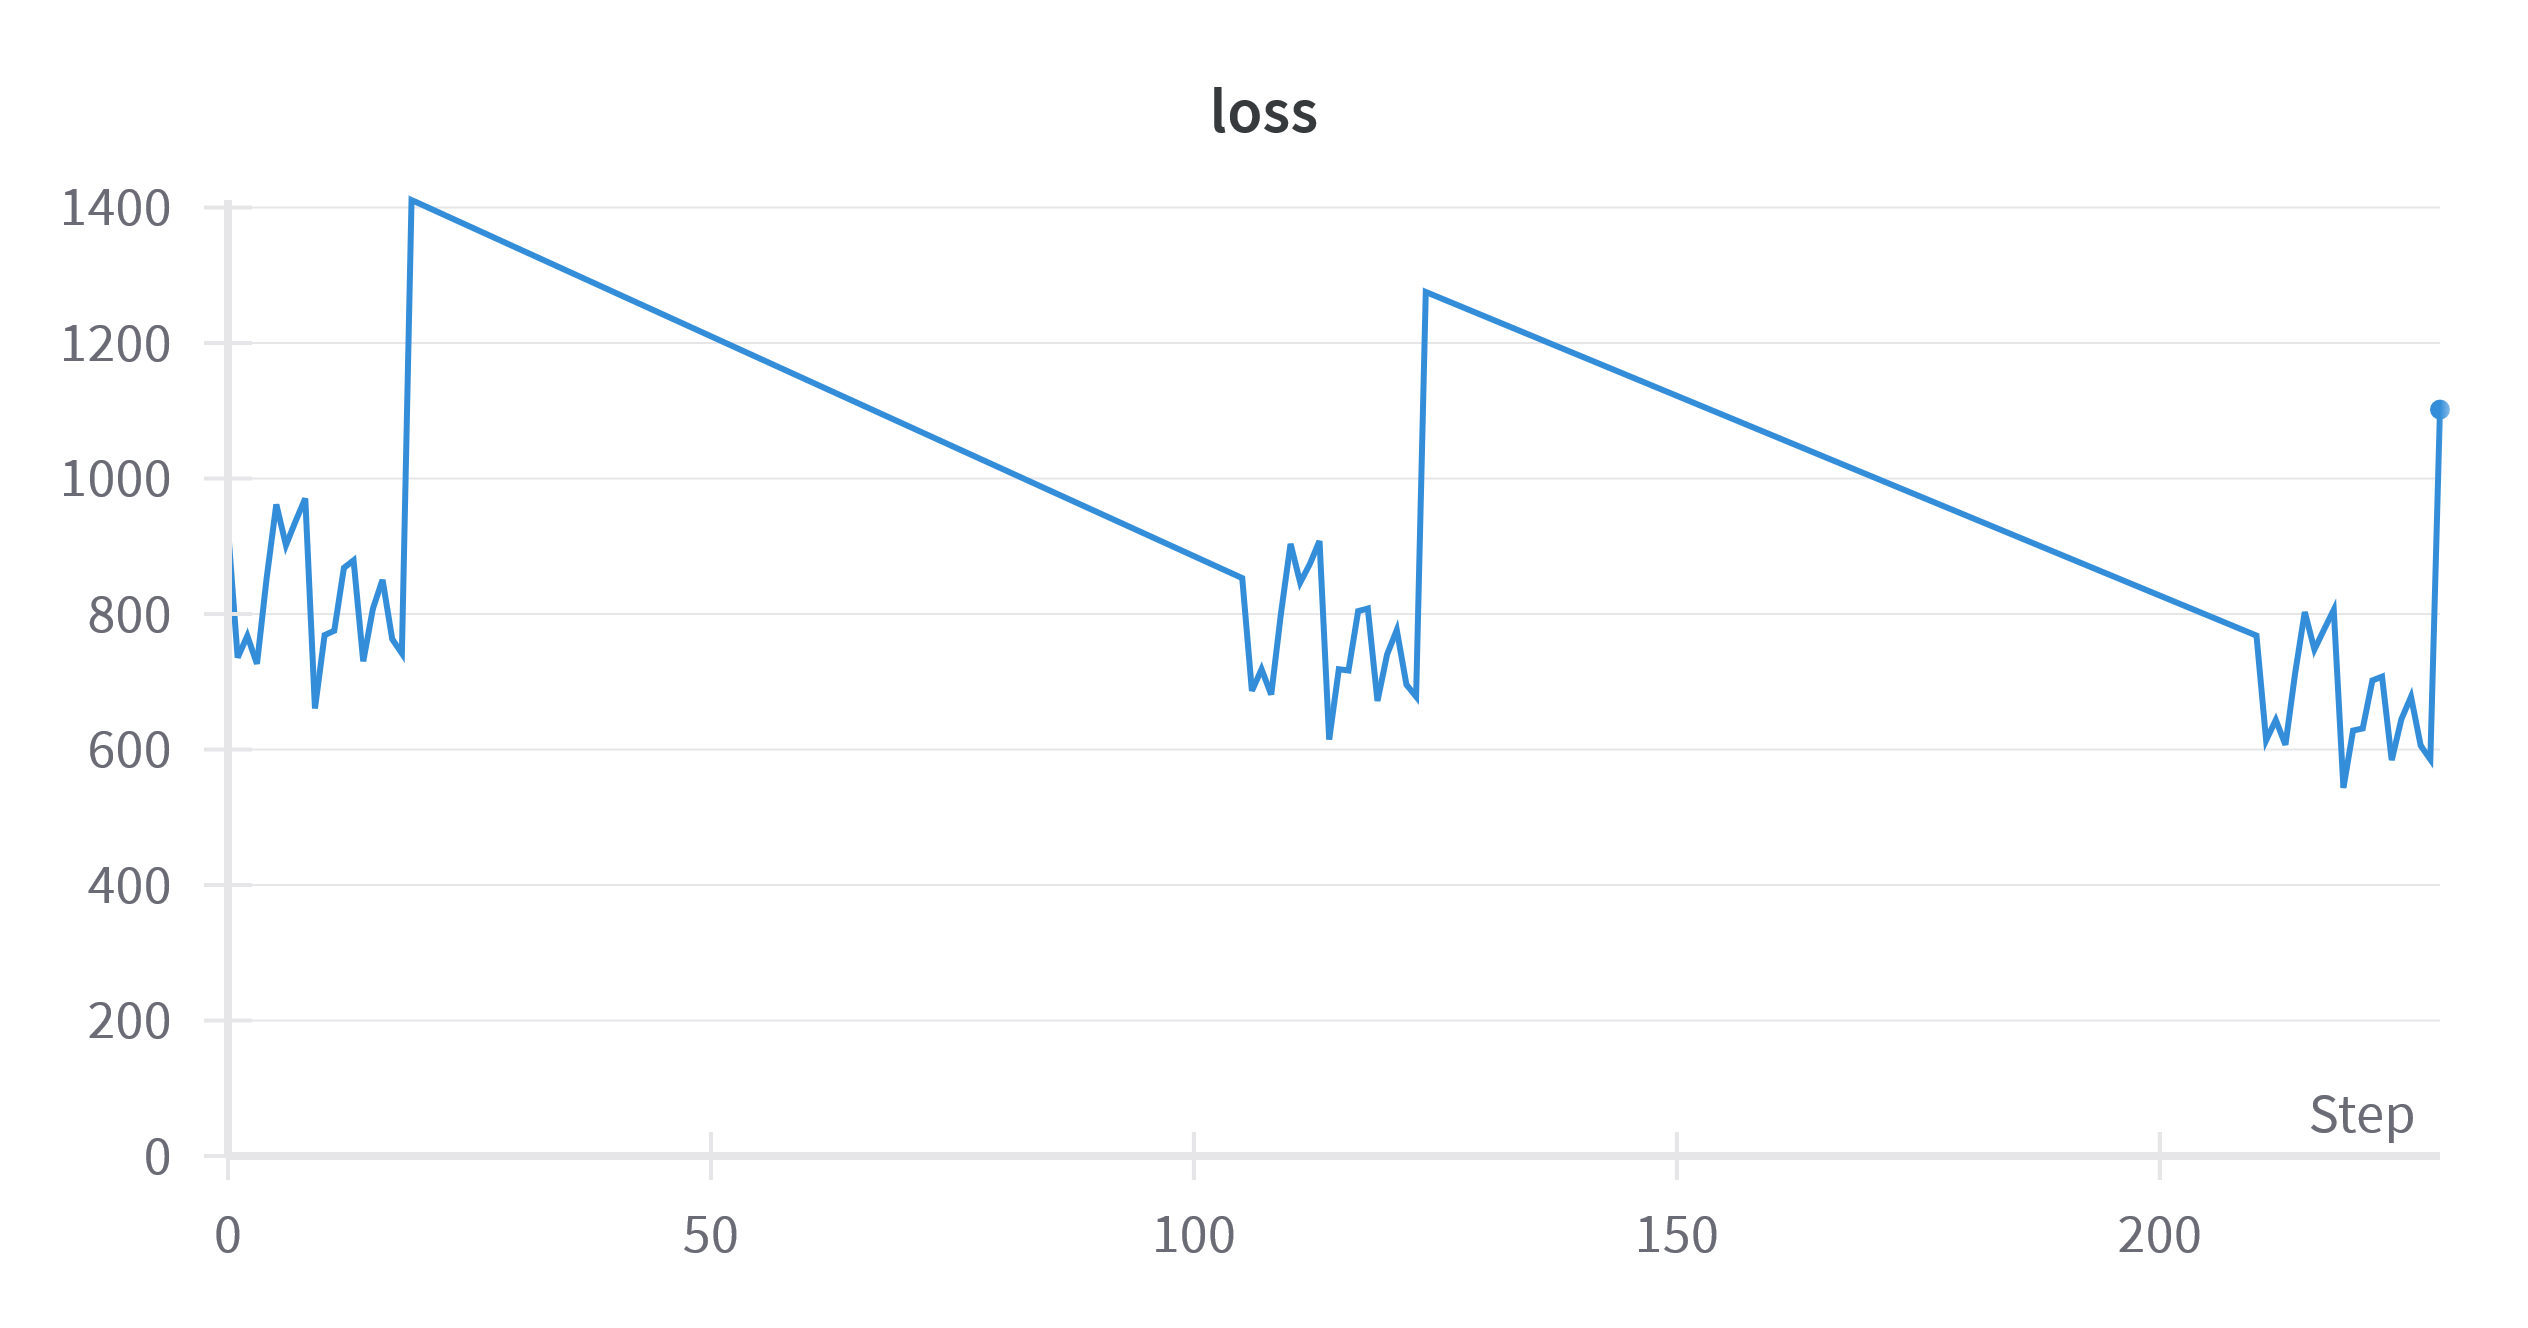
\includegraphics[width=0.45\linewidth]{figures/Figure25.png}}
    \subfigure[Test loss]{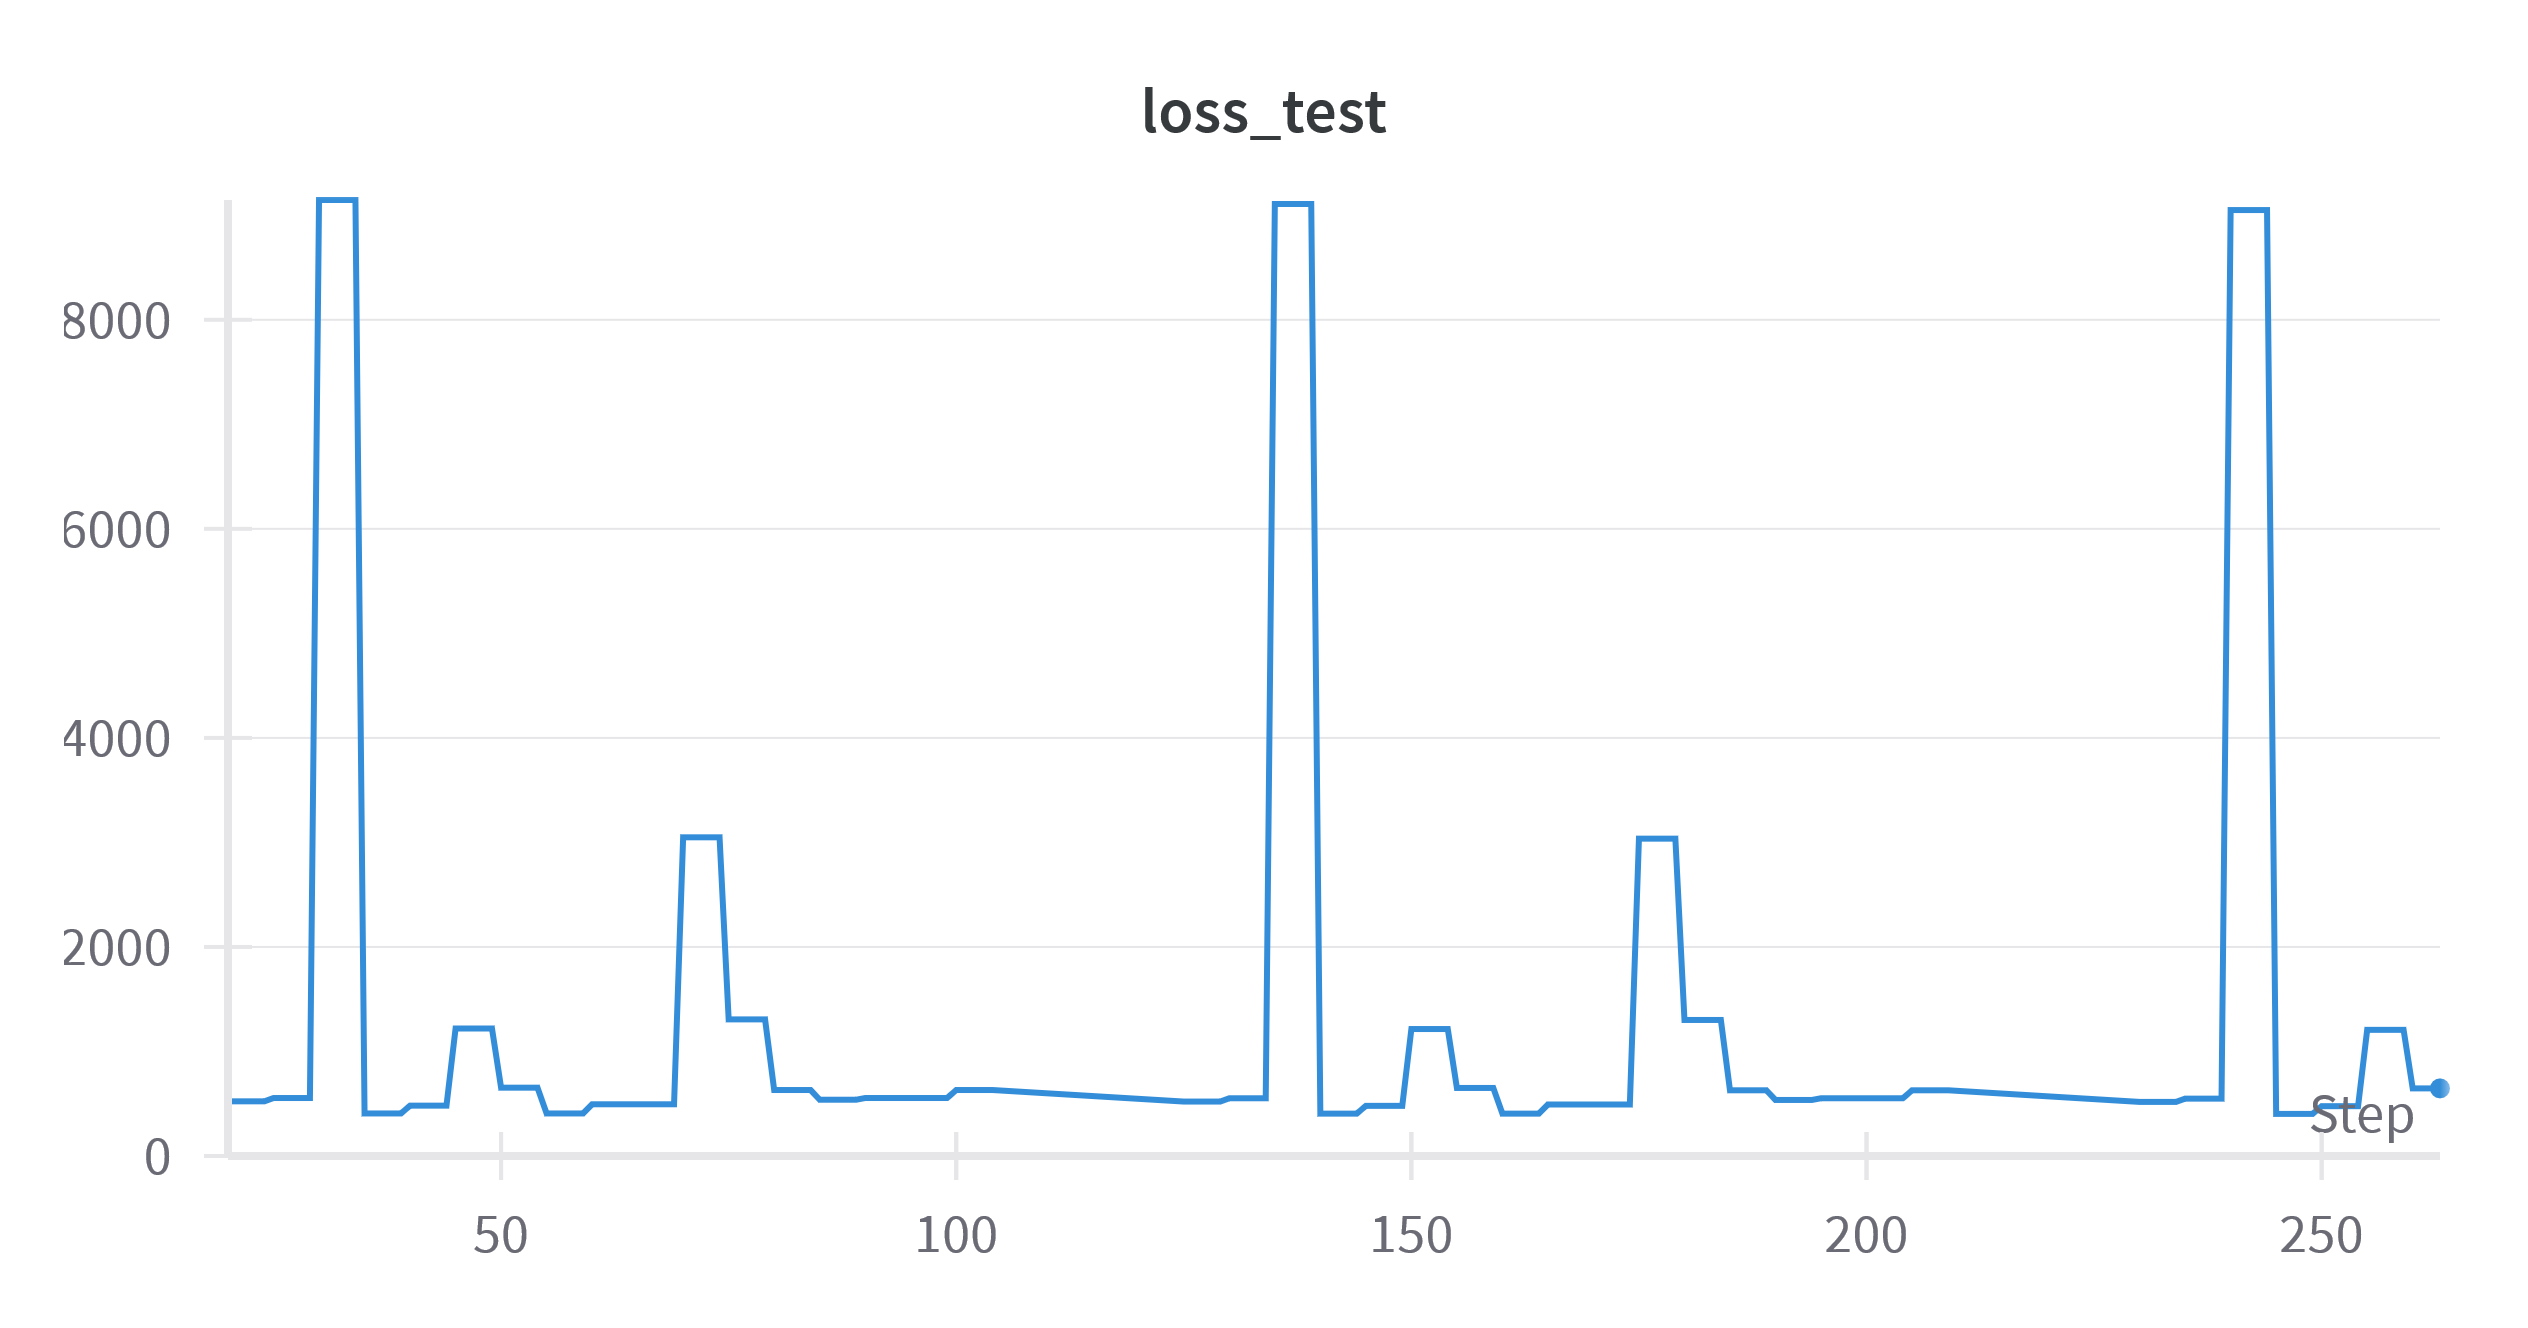
\includegraphics[width=0.45\linewidth]{figures/Figure26.png}}
    \caption{Loss graphs for the EfficientDet D-0 model trained on train and then test sets}
    \label{fig:fig23}
\end{figure}

\subsection{Experiment 2}

The figure does not indicate any loss reduction, so I changed the configuration of the detector. I chose not to normalize the images, each of size 3$\times$512$\times$512 and test how the model behaves. I also discovered that EfficientDet works better when the bounding box coordinates are given in (y,x,y,x) order, and so I changed it from (x, y, width, height). Additionally, I used pre-trained weights, which I obtained from Alex Shonenkov's Kaggle account ~\cite{link6} and I reset both the classification head and the regression head in order to fit my classification problem. 

The hyper-parameters are the same as in the previous experiment. The model was trained for one epoch; I stopped the run before it had a chance to validate the model, so there is no graph for the test loss. Figure \ref{fig:fig24} shows the train loss.

\begin{figure}[!ht]
    \centering
    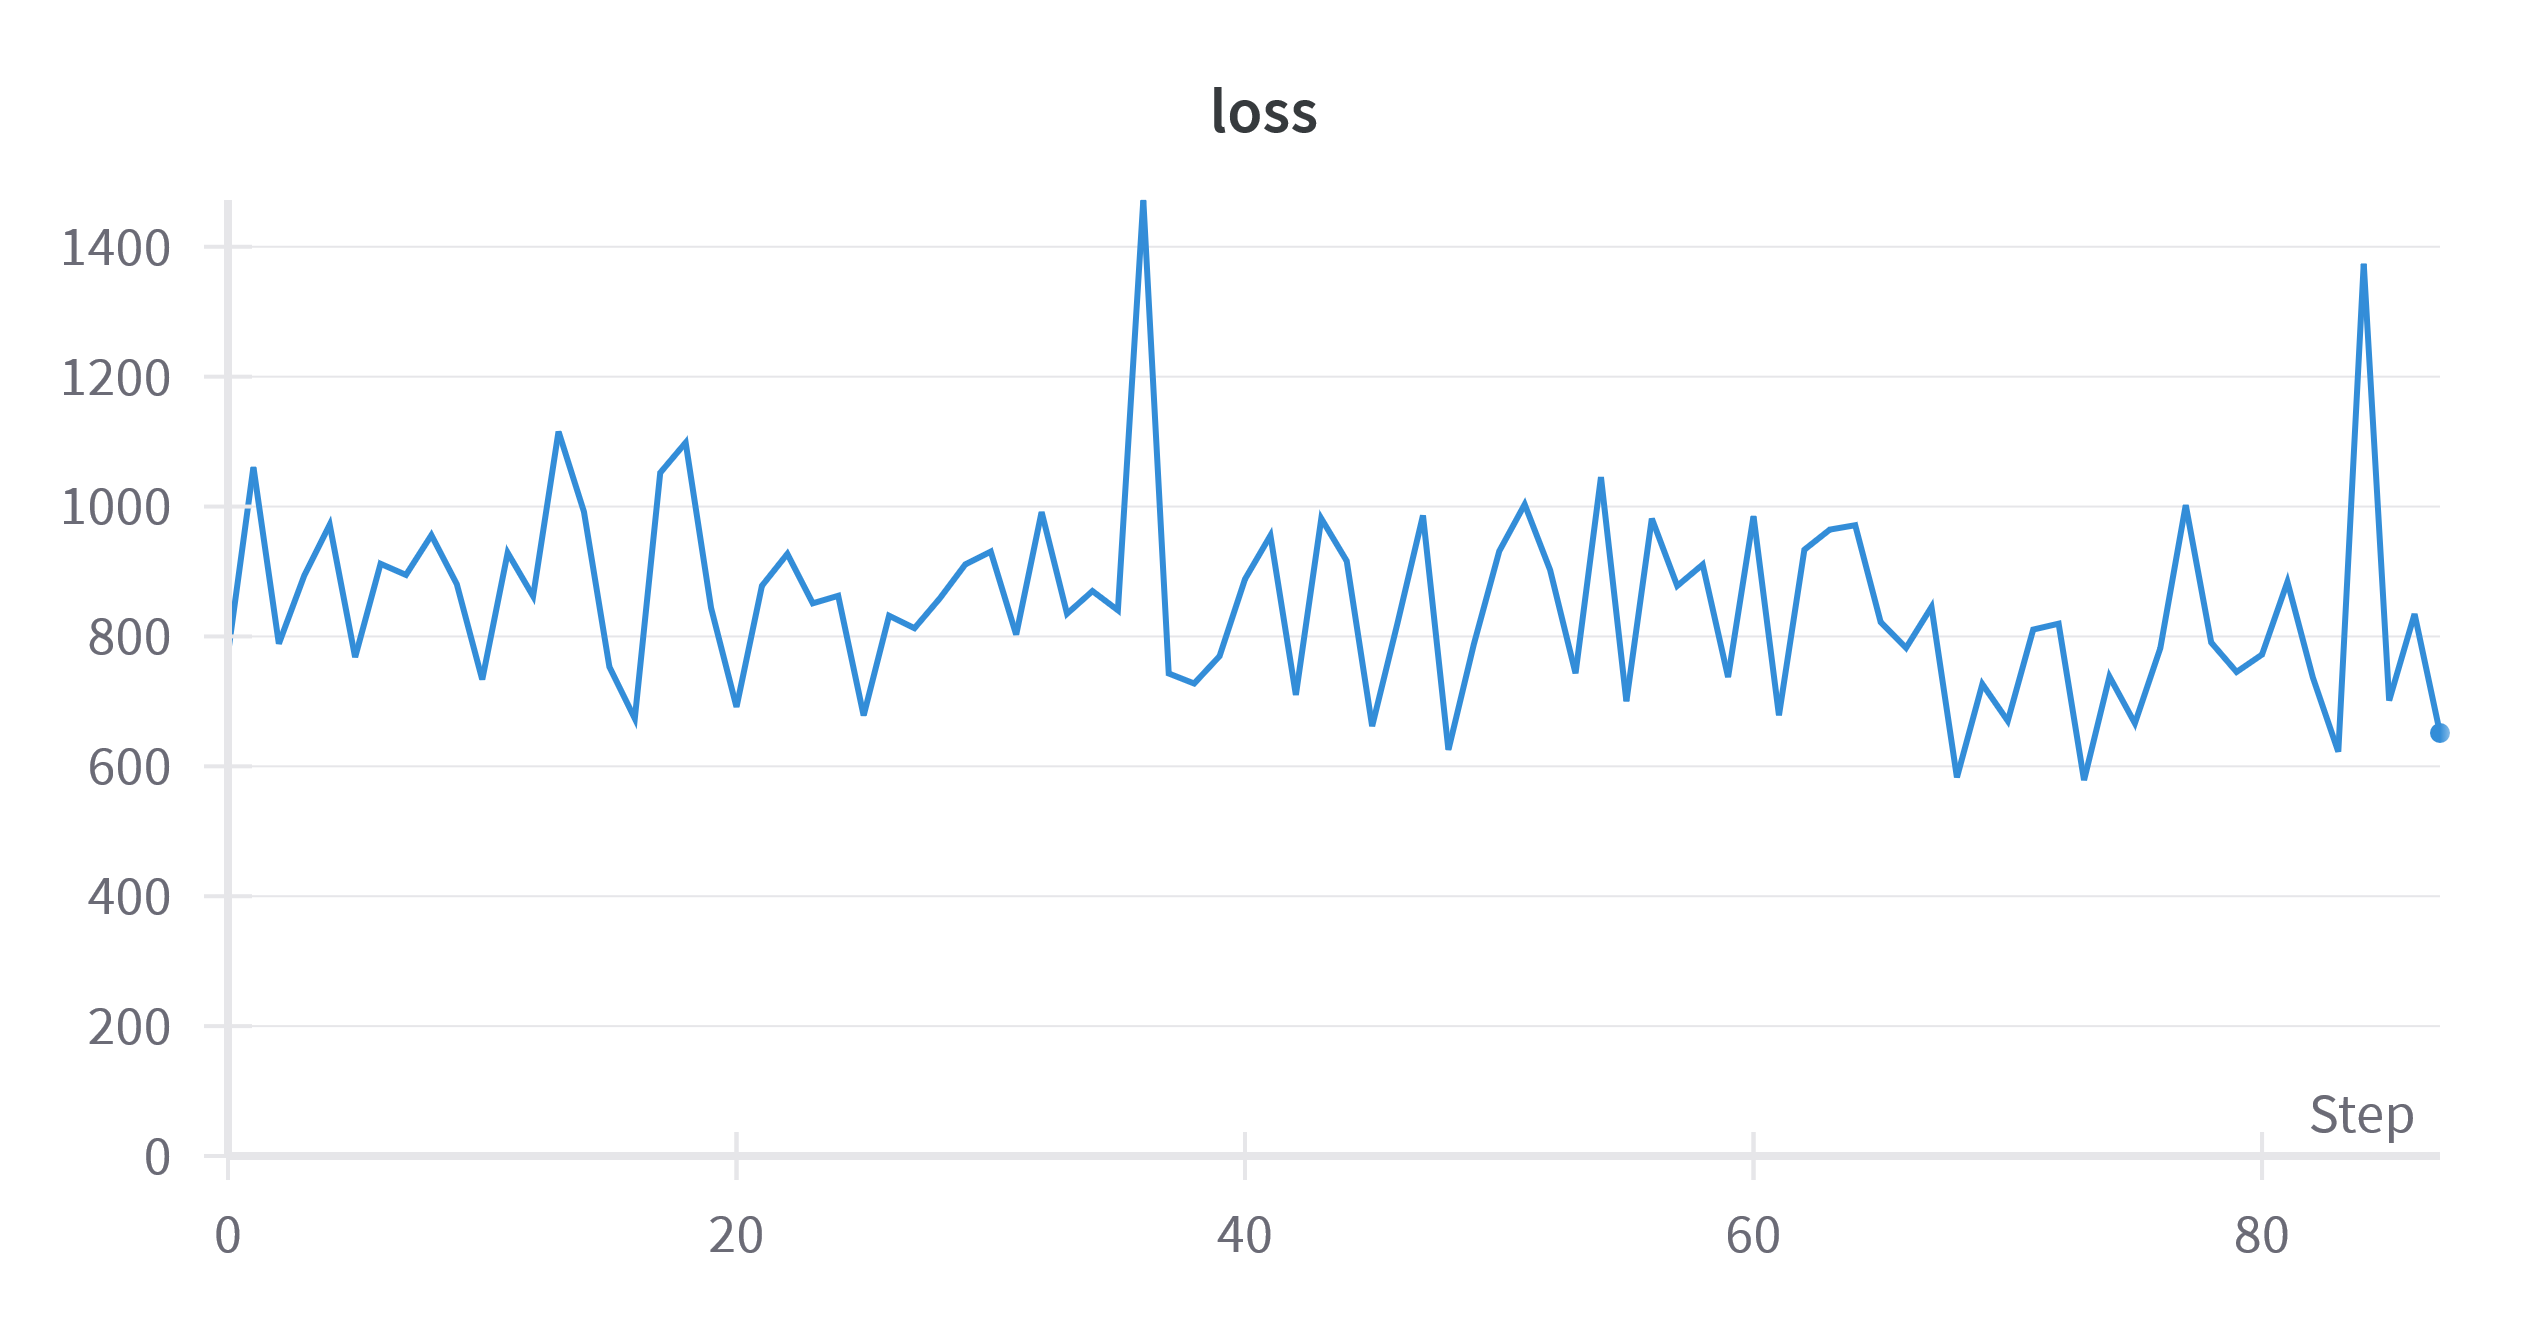
\includegraphics[width=1\linewidth]{figures/Figure27.png}
    \caption{Loss Graph on train set using the original EfficientDet with pre-trained weights from Kaggle code}
    \label{fig:fig24}
\end{figure}

I took the same configuration and trained it for 50 epochs to see how the loss evolved. Instead of running the train loop once for 50 epochs, I ran the loop five times with 10 epochs each. Because of this, the graph is not continuous; each batch of 10 epochs starts at the 0 step, but each batch after the first one starts with the weights trained from the previous batches.
 
In the first 10 epochs, shown in figure \ref{fig:fig25}, the loss decrease is steep, and so is the test loss. However, after 40 epochs, the decline gets more gradual, as shown in figure \ref{fig:fig26}.

\begin{figure}[H]
    \subfigure[Train loss]{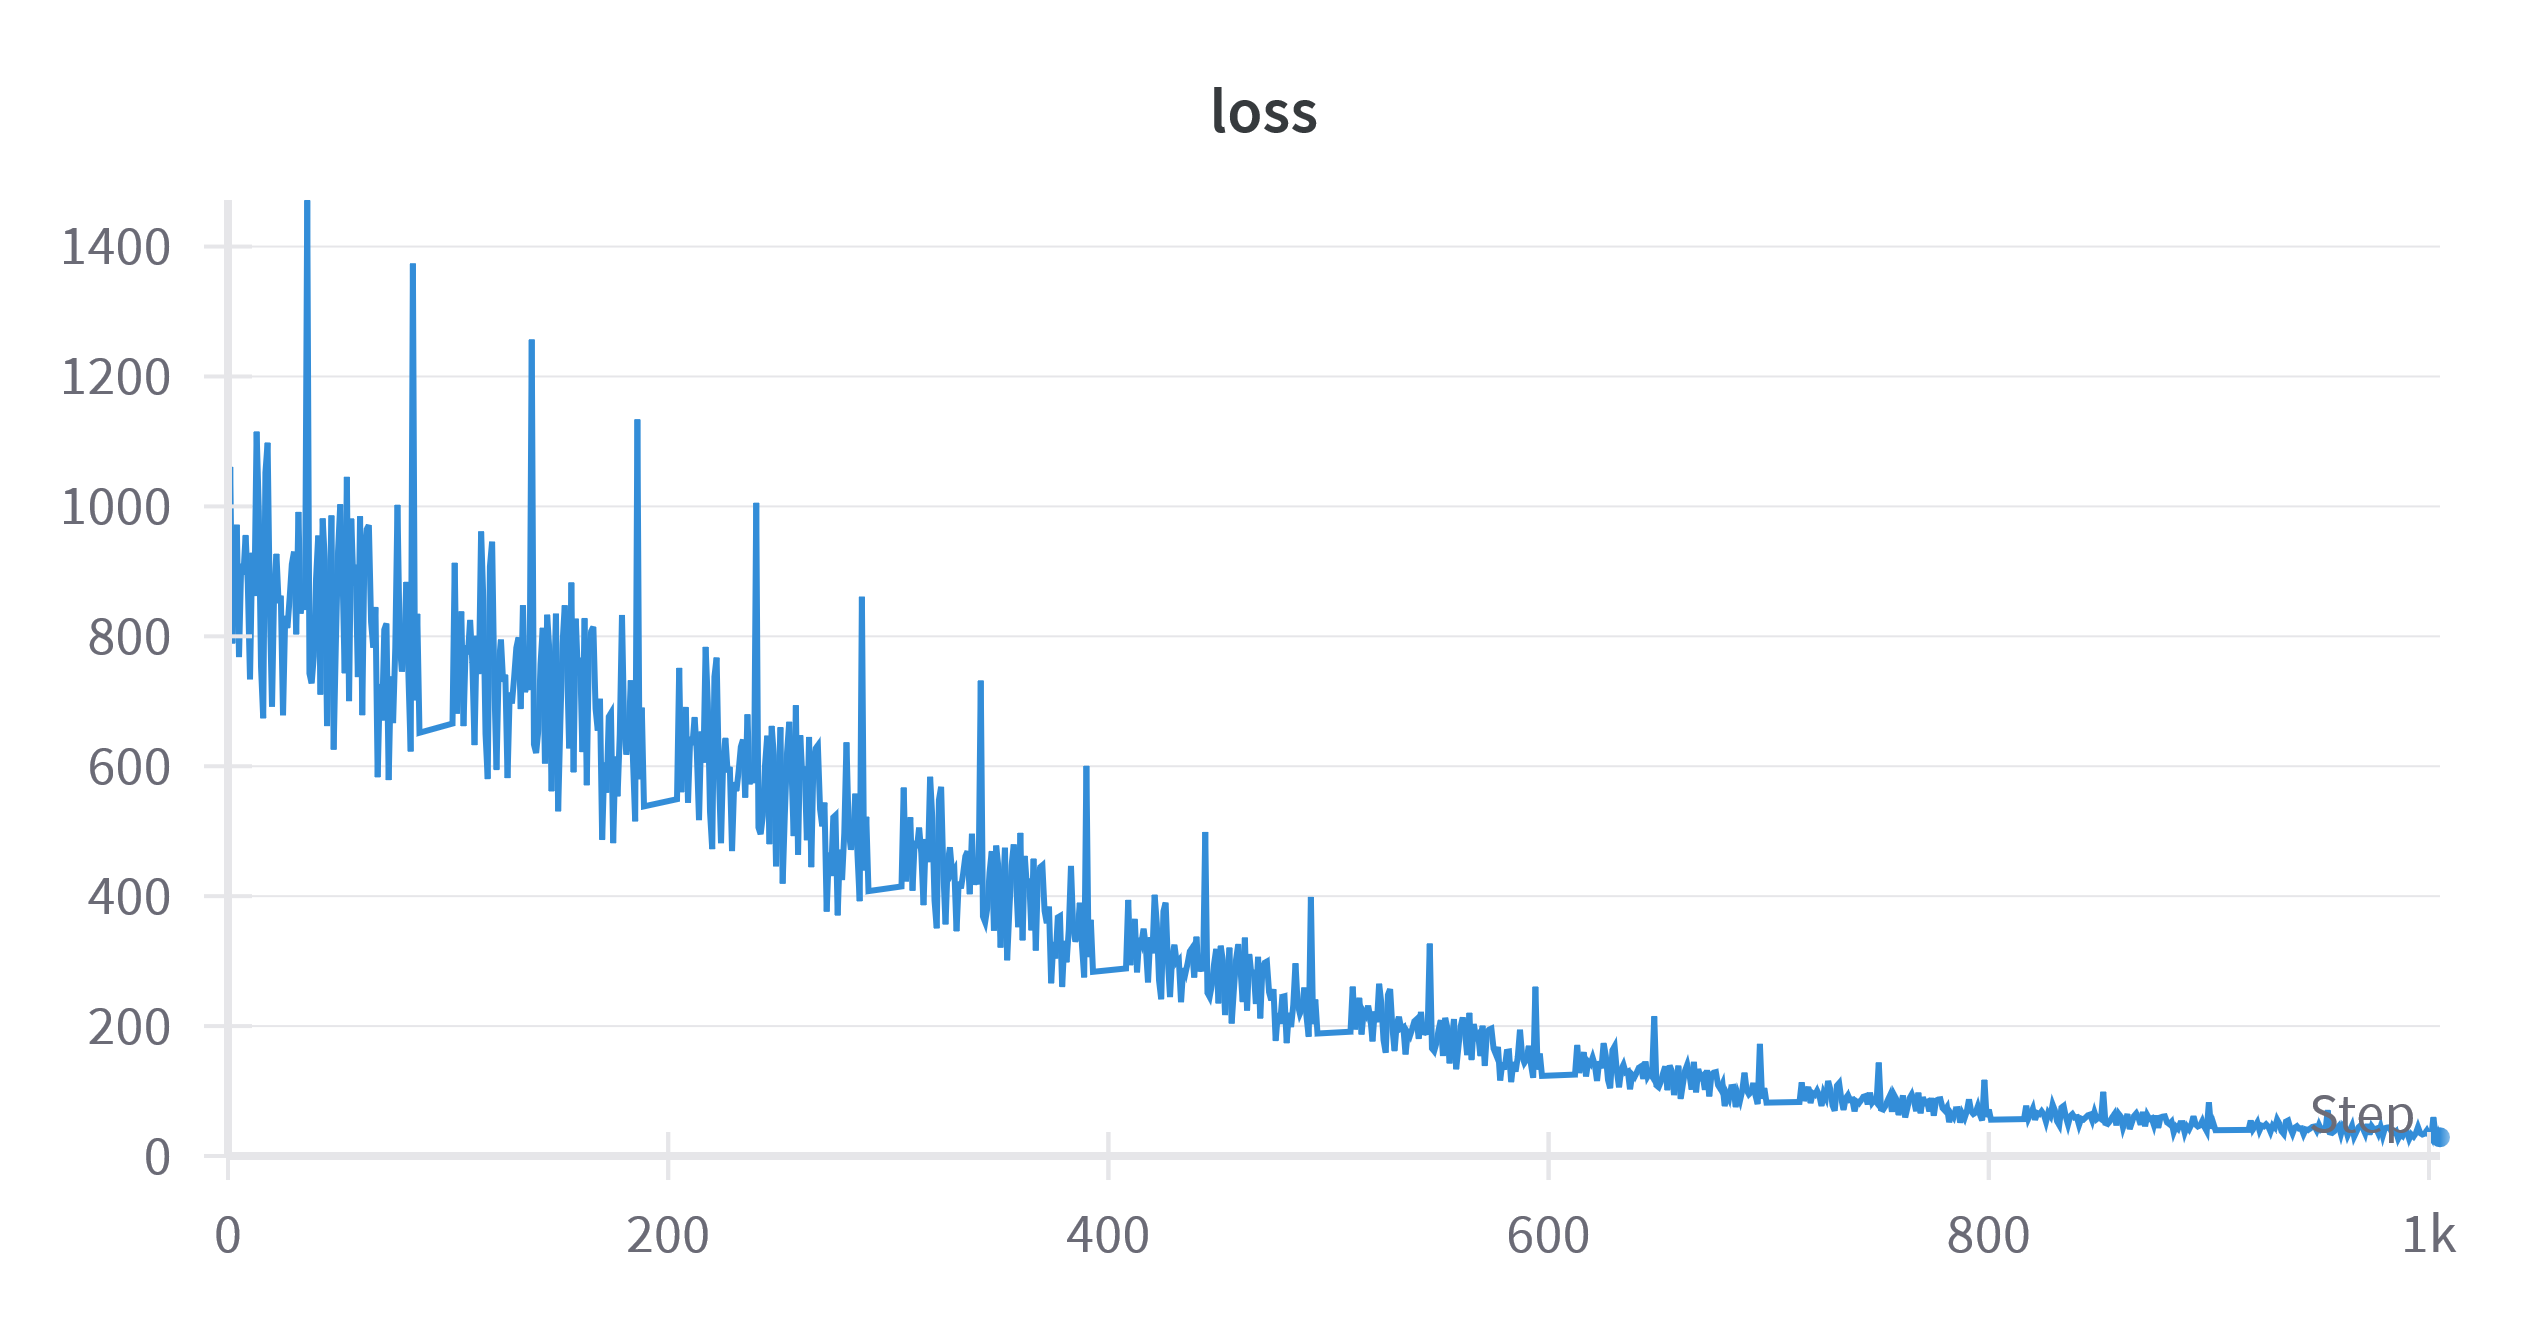
\includegraphics[width=0.45\linewidth]{figures/Figure28.png}}
    \subfigure[Test loss]{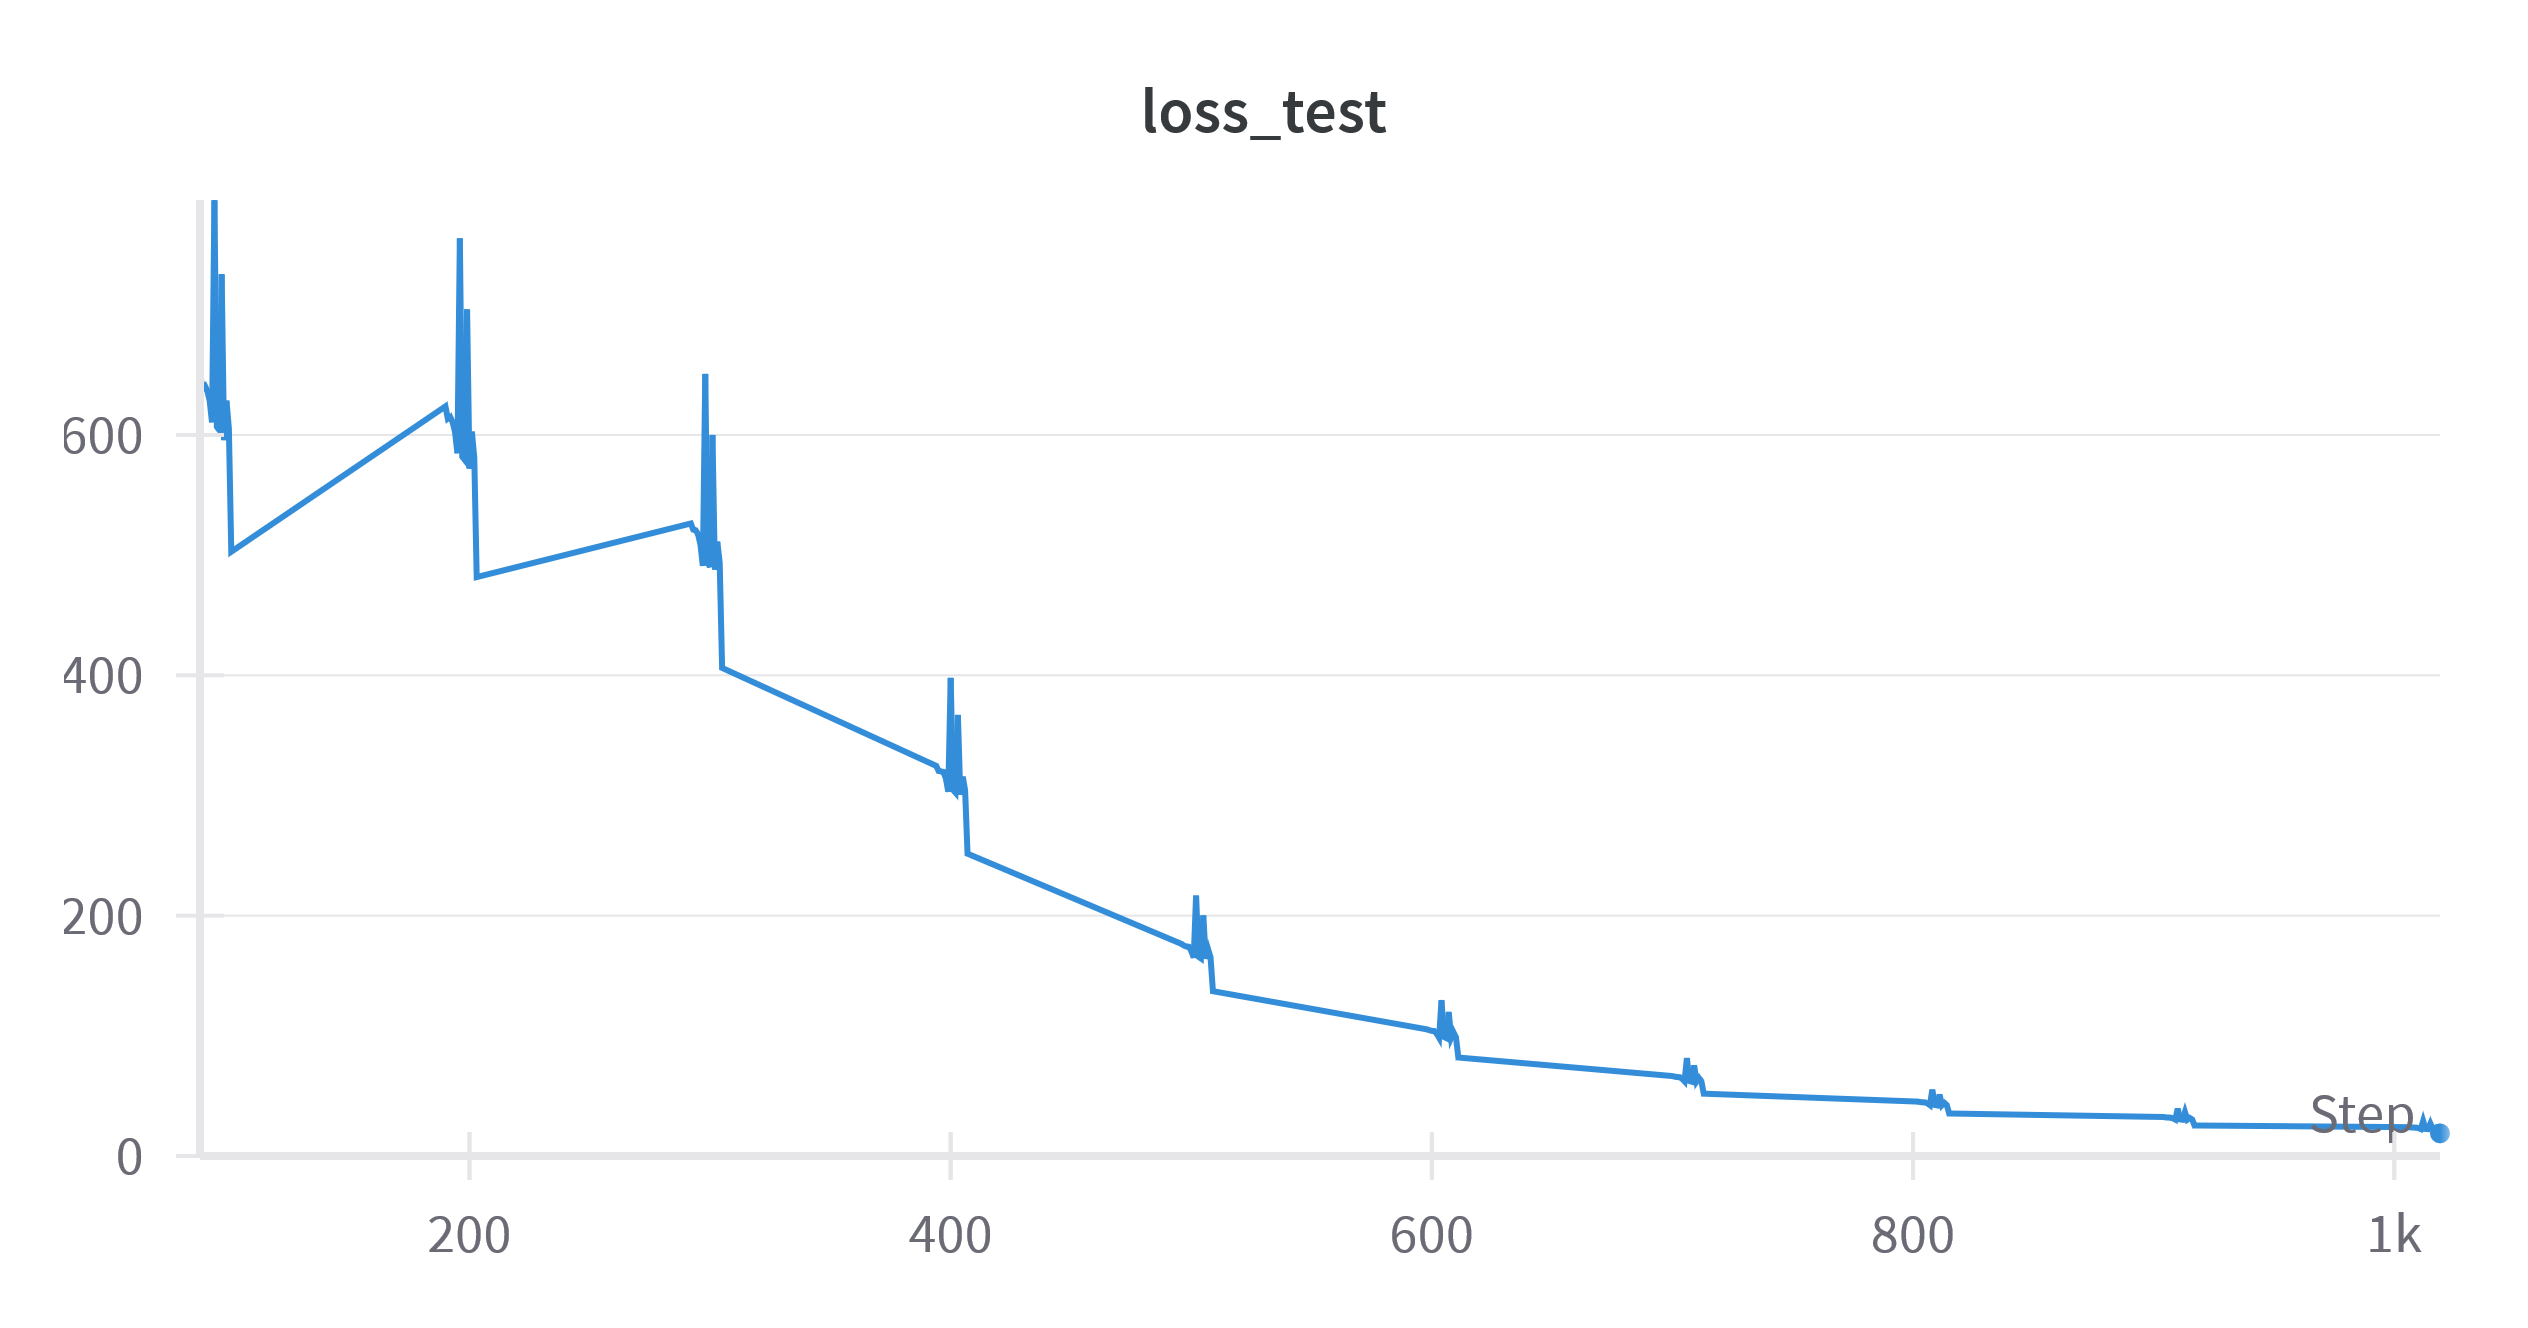
\includegraphics[width=0.45\linewidth]{figures/Figure29.png}}
    \caption{Loss graphs for the original EfficientDet D-0 model with pre-trained weights from Kaggle code trained on train and then test sets after 10 epochs}
    \label{fig:fig25}
\end{figure}

\begin{figure}[H]
    \subfigure[Train loss]{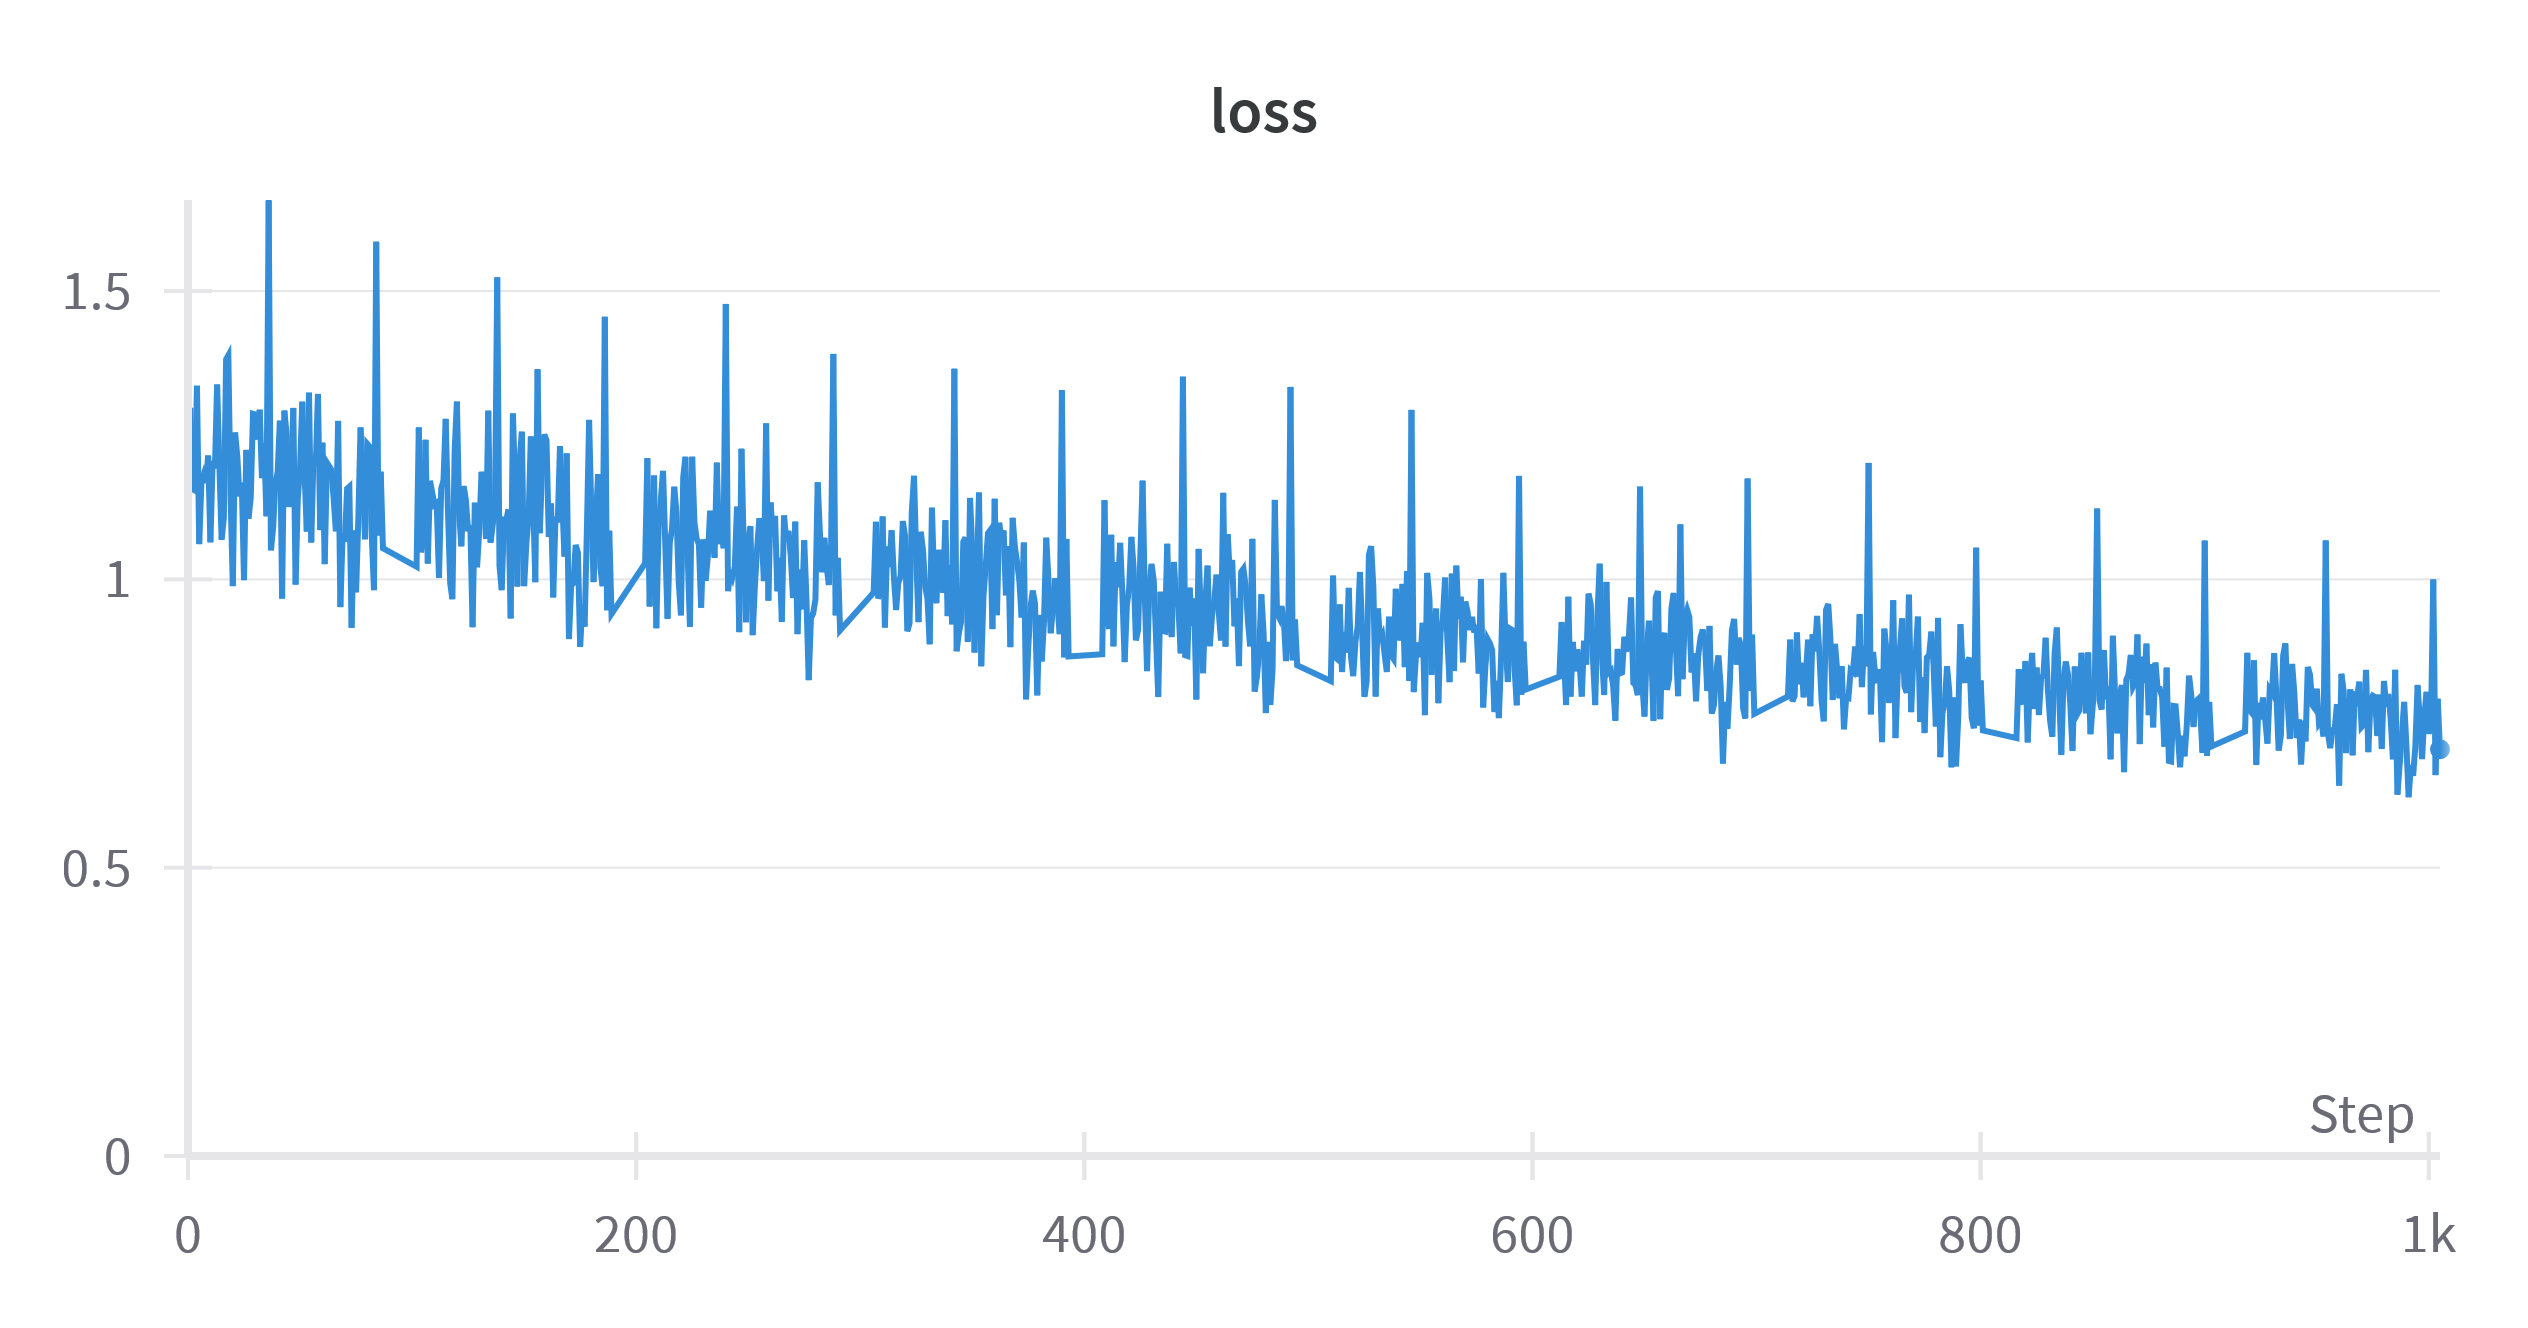
\includegraphics[width=0.45\linewidth]{figures/Figure30.png}}
    \subfigure[Test loss]{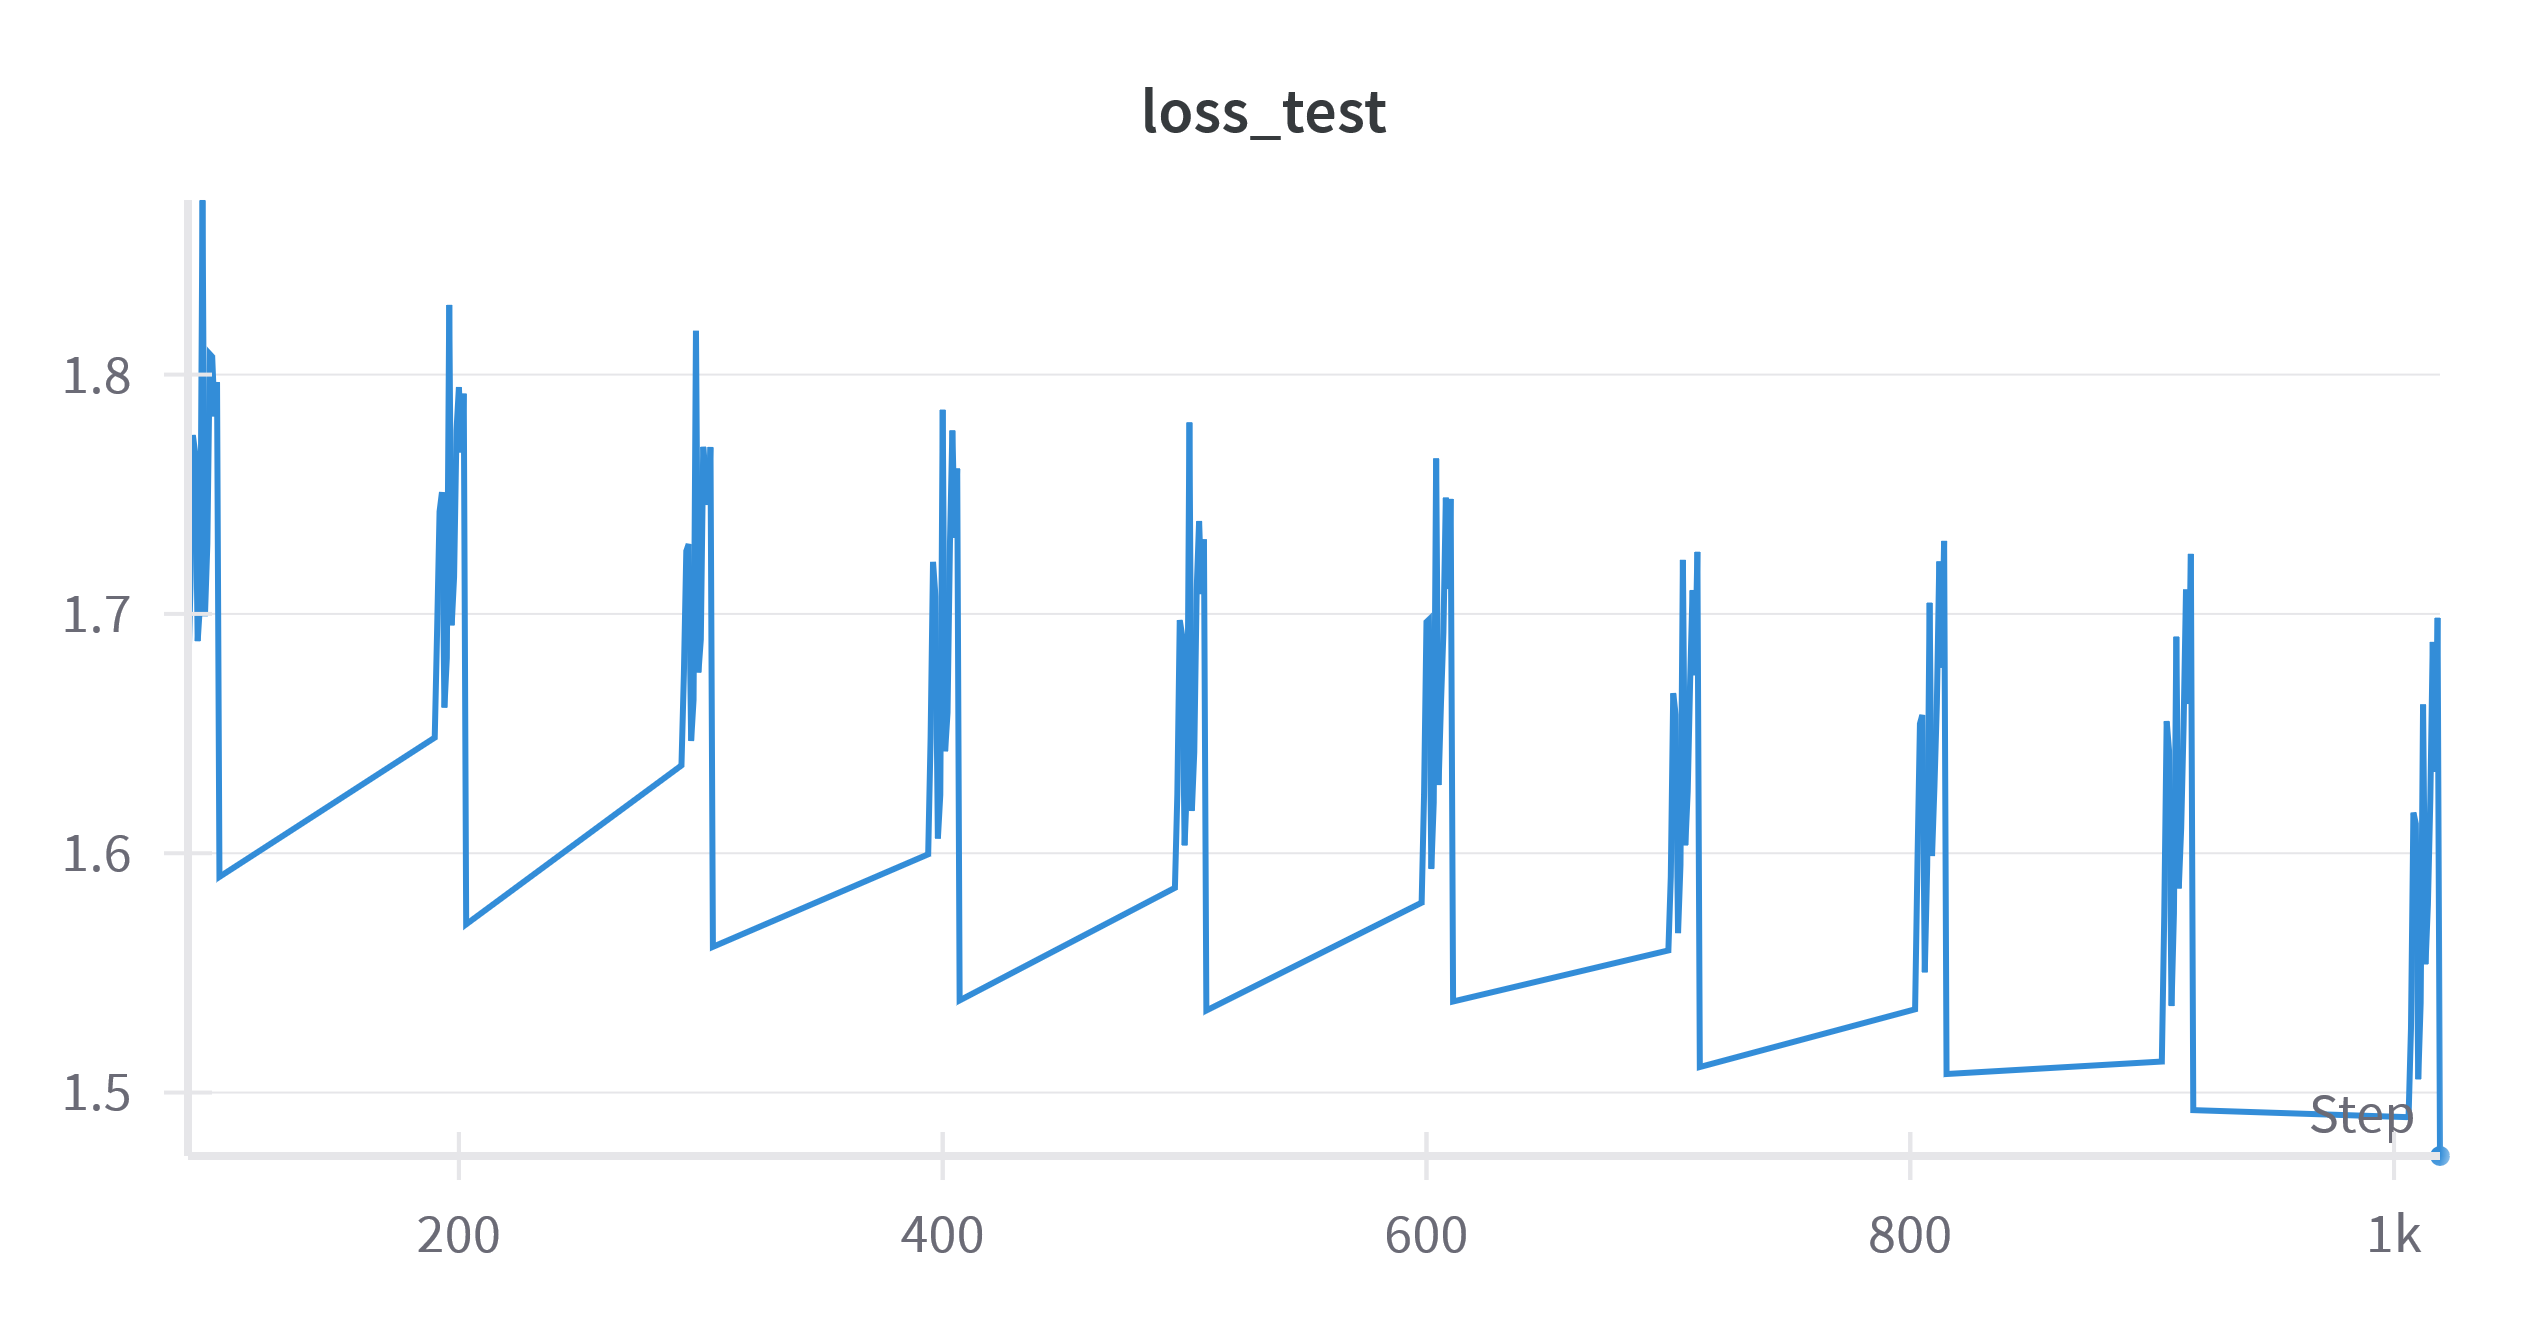
\includegraphics[width=0.45\linewidth]{figures/Figure31.png}}
    \caption{Loss graphs for the original EfficientDet D-0 model with pre-trained weights from Kaggle code trained on train and then test sets after 40 epochs}
    \label{fig:fig26}
\end{figure}

\subsection{Experiment 3}

For the next experiment, I normalized the images again to see if I could get a starting loss lower than the previous ones. I also found another file containing pre-trained weights, this time from the official Effdet library on GitHub ~\cite{link7}. With this configuration, I trained all the layers for 13 epochs. The hyper-parameters remained the same as in the previous experiments. 

Figure \ref{fig:fig27} shows how the train and test loss looked after those 13 epochs. While the initial loss was much lower than the previous ones, I was not satisfied with the test loss, so I continued to experiment.

\begin{figure}[!ht]
    \subfigure[Train loss]{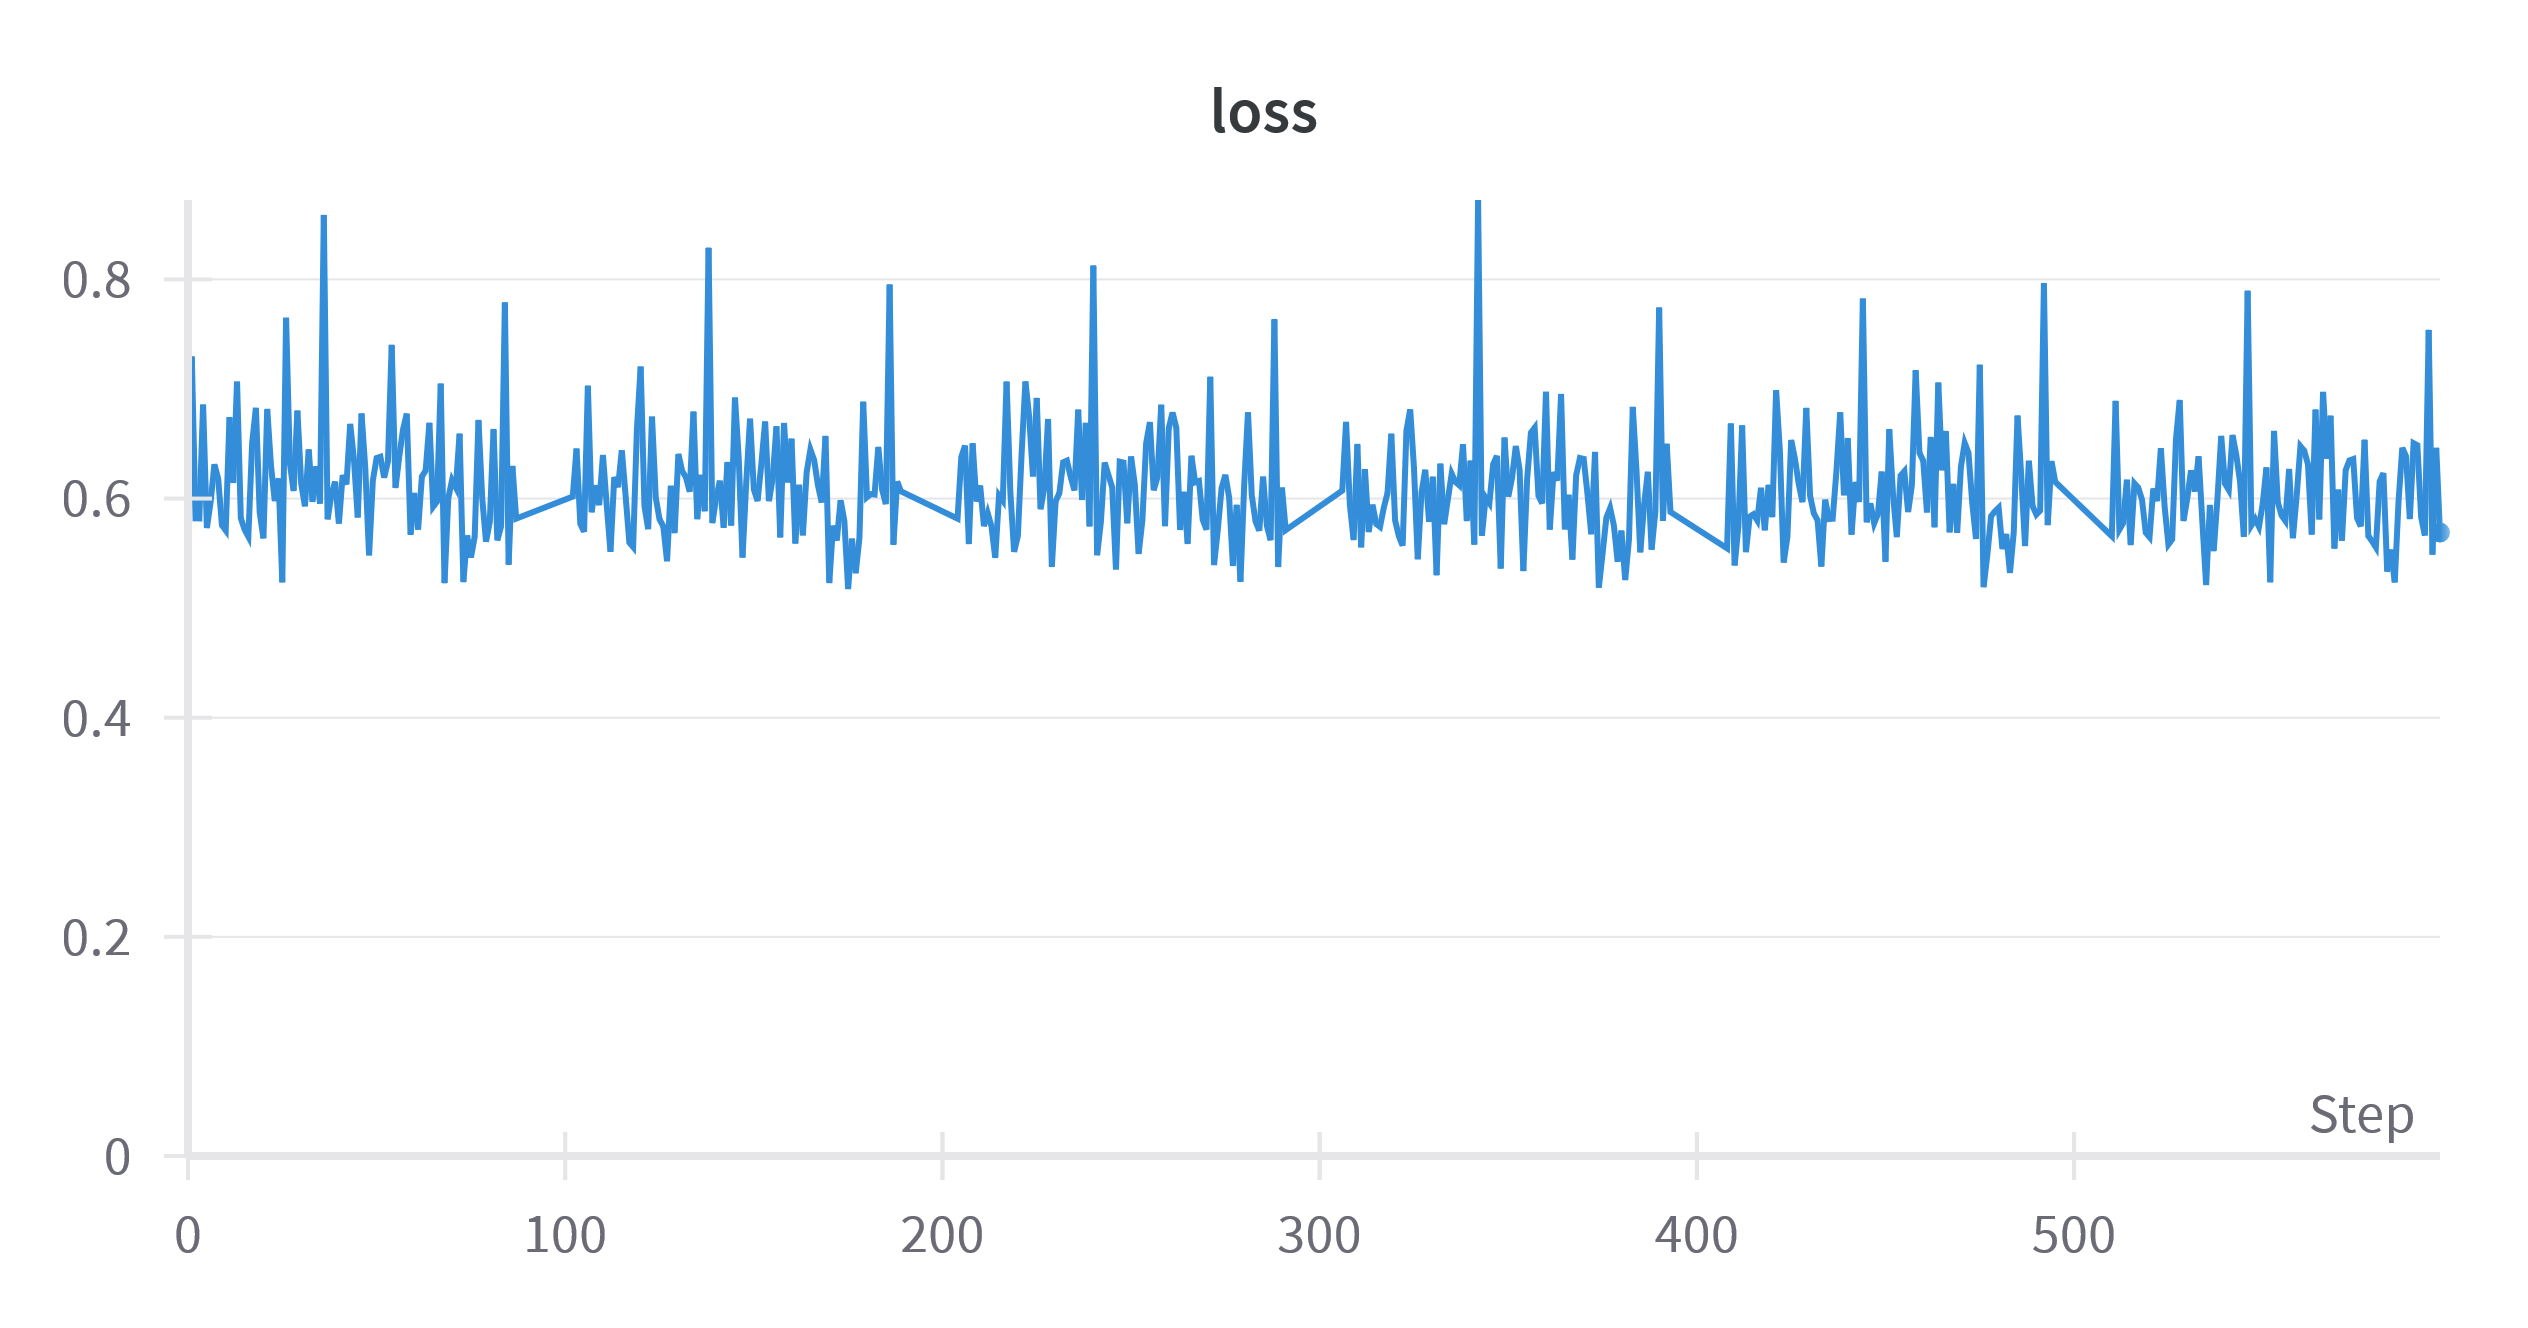
\includegraphics[width=0.45\linewidth]{figures/Figure32.png}}
    \subfigure[Test loss]{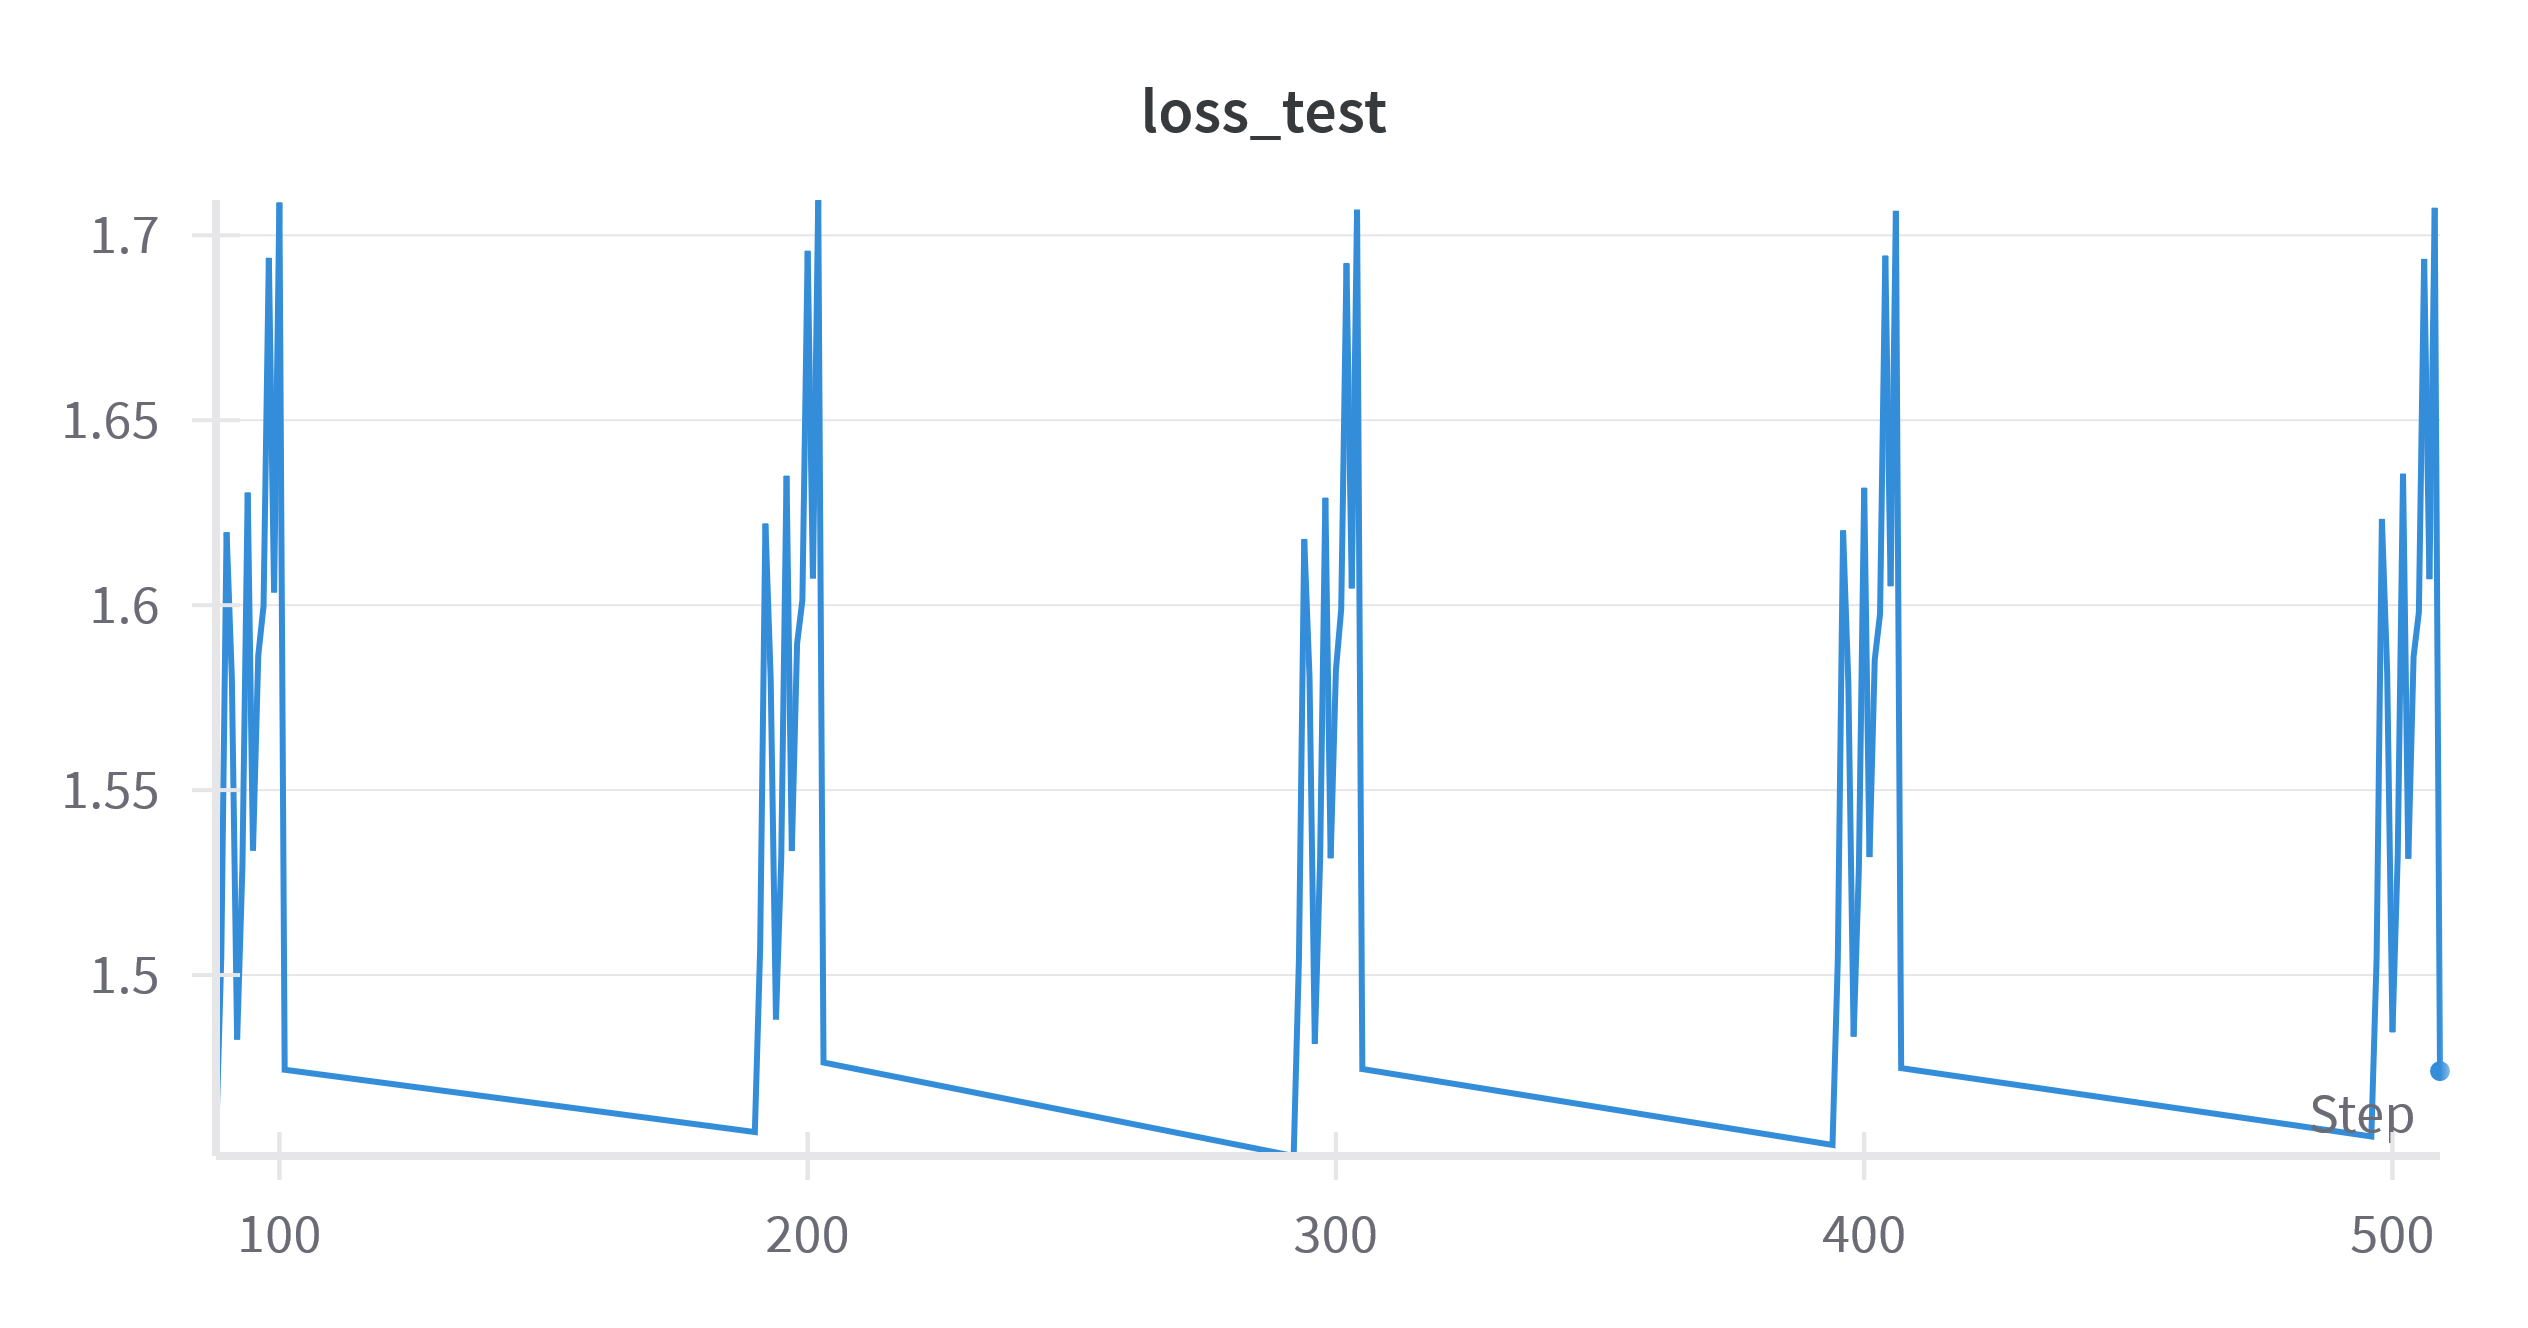
\includegraphics[width=0.45\linewidth]{figures/Figure33.png}}
    \label{fig:fig27}
    \caption{Loss graphs for the original EfficientDet D-0 model with pre-trained weights from the official GitHub account without anchors trained on train and then test sets}
\end{figure}

\subsection{Experiment 4}

In the next experiment, I changed the learning rate decay from ReduceLROnPlateau to CosineAnnealingLR, with a minimum learning rate of $1e^{-6}$. I also modified the way the decay is applied, calling it after each step in the train loop and using the loss as a metric rather than the test. Additionally, I modified the way the model is initialized; instead of manually downloading the file and loading a Pytorh script, I used the create\_model\_from\_config method from the Effdet library, calling it this way: \[
create\_model\_from\_config(bench\_task='train', num\_classes=2, pretrained=True)\]

I also trained this model for 50 epochs in the same way as experiment 3. Figure \ref{fig:fig12} shows how the train and test looked for the first 10 epochs, and figure \ref{fig:fig14} shows how the train and test looked for the 40 to 50 epochs.

\begin{figure}[!ht]
    \subfigure[Train loss]{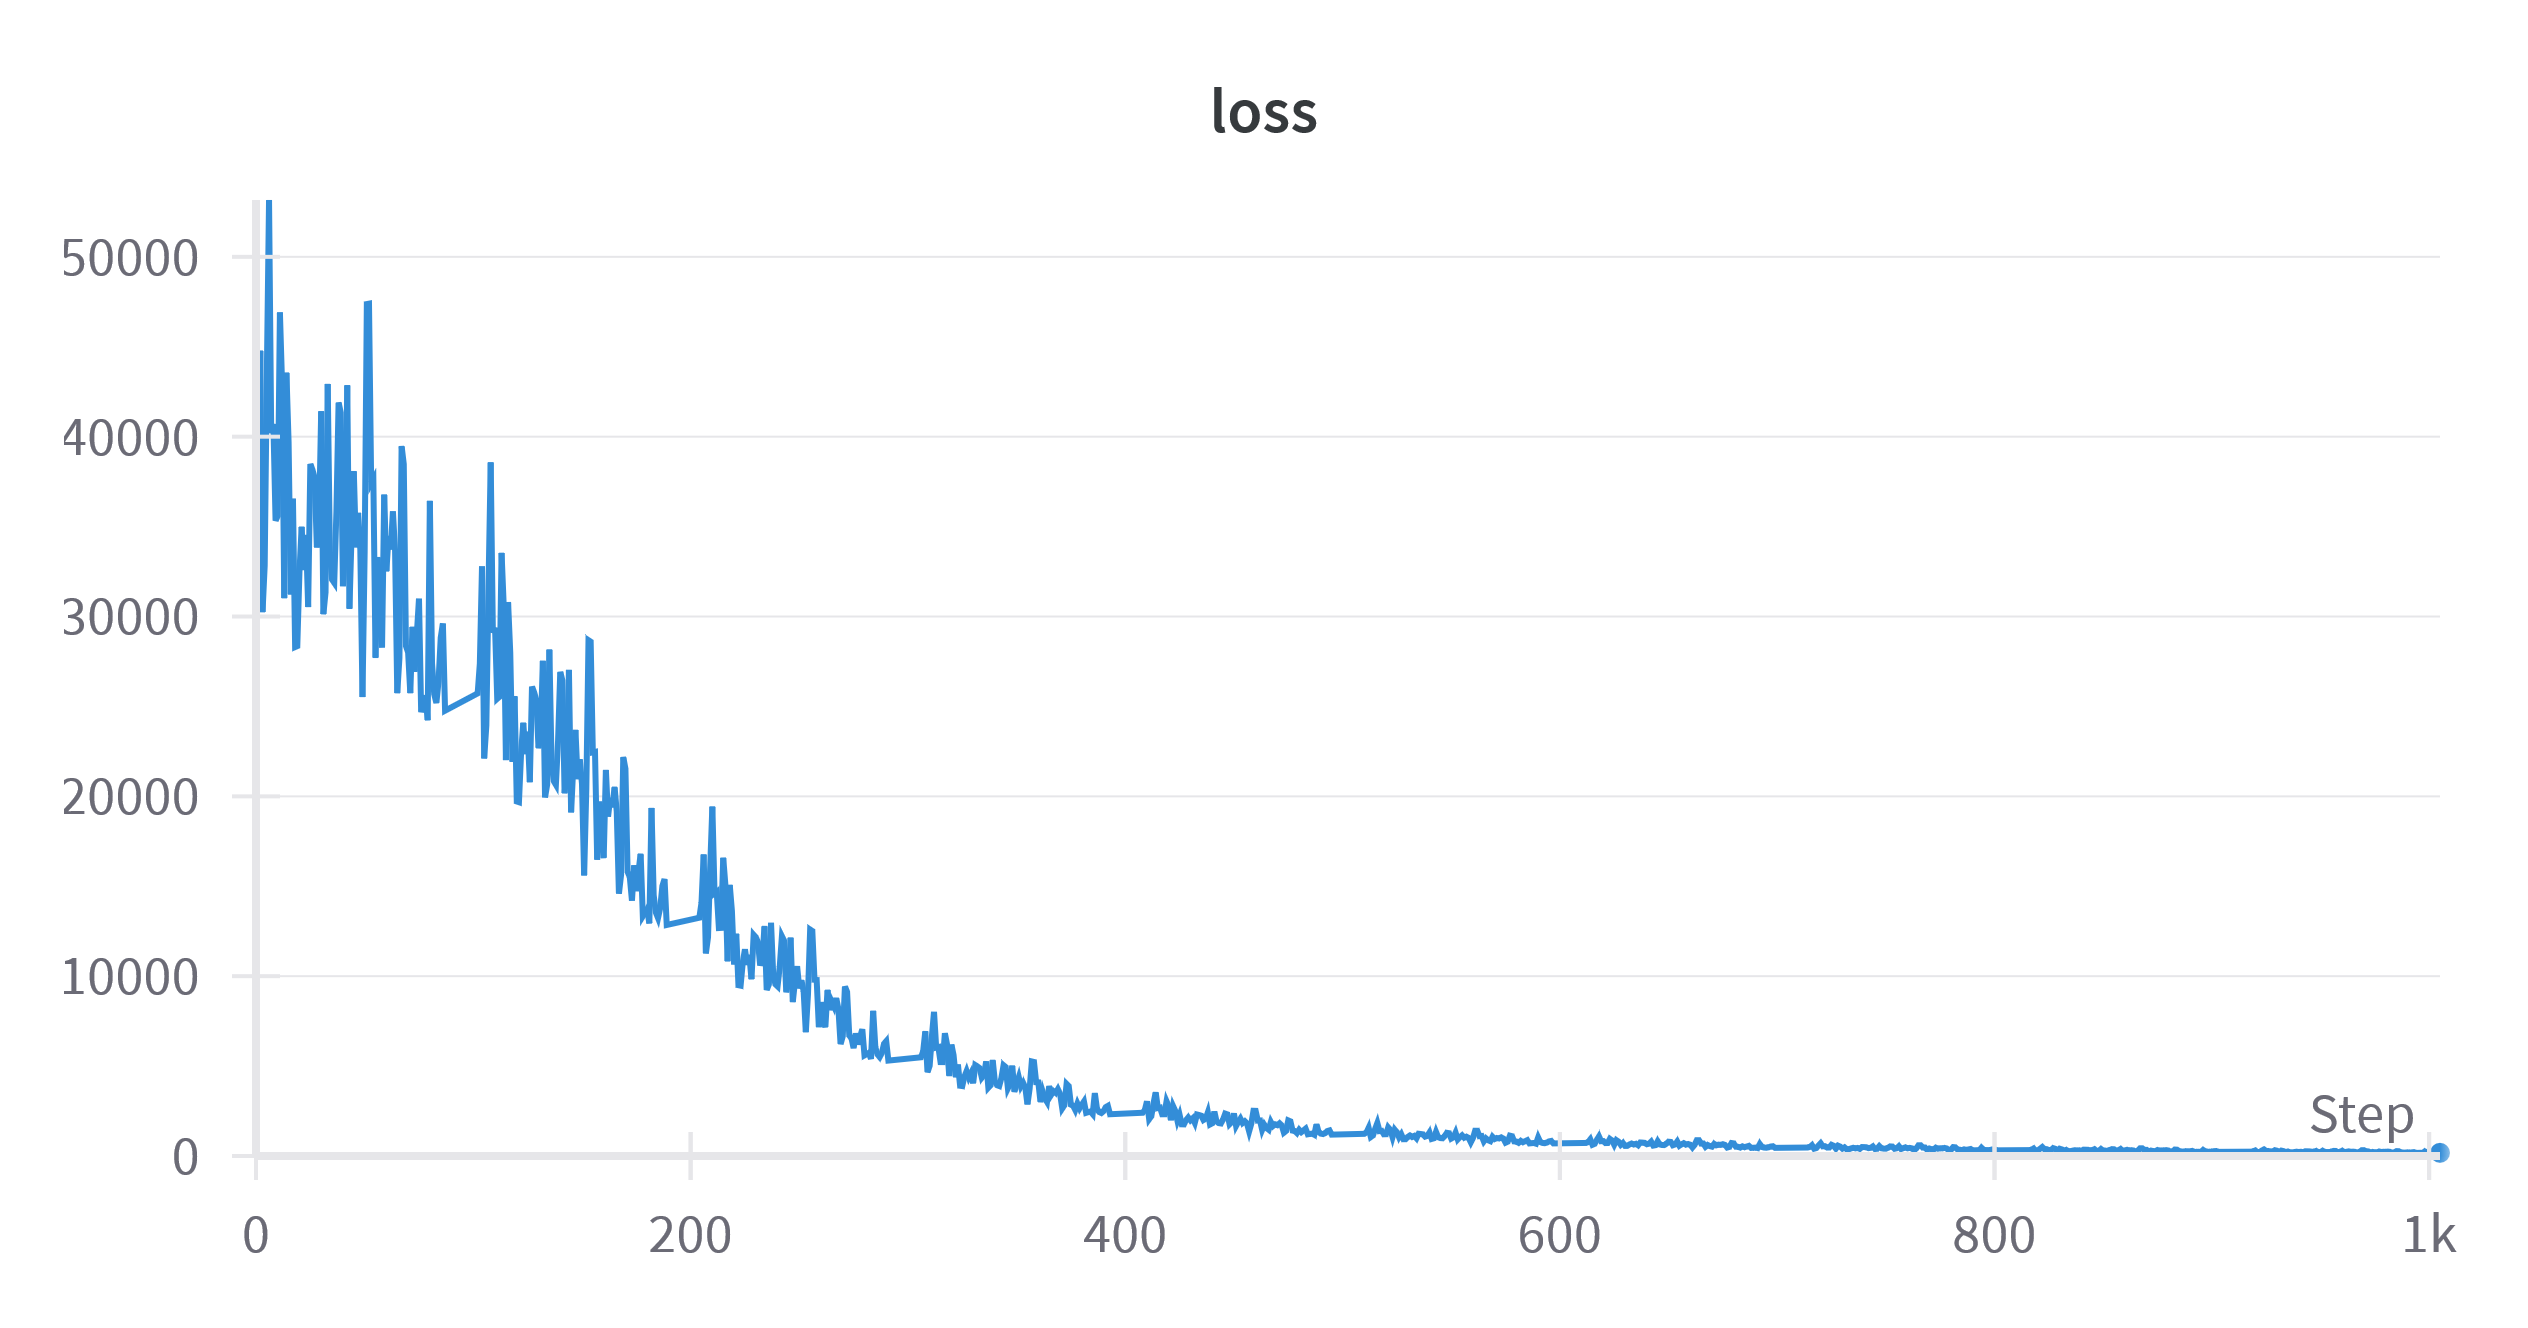
\includegraphics[width=0.45\linewidth]{figures/Figure23.png}}
    \subfigure[Test loss]{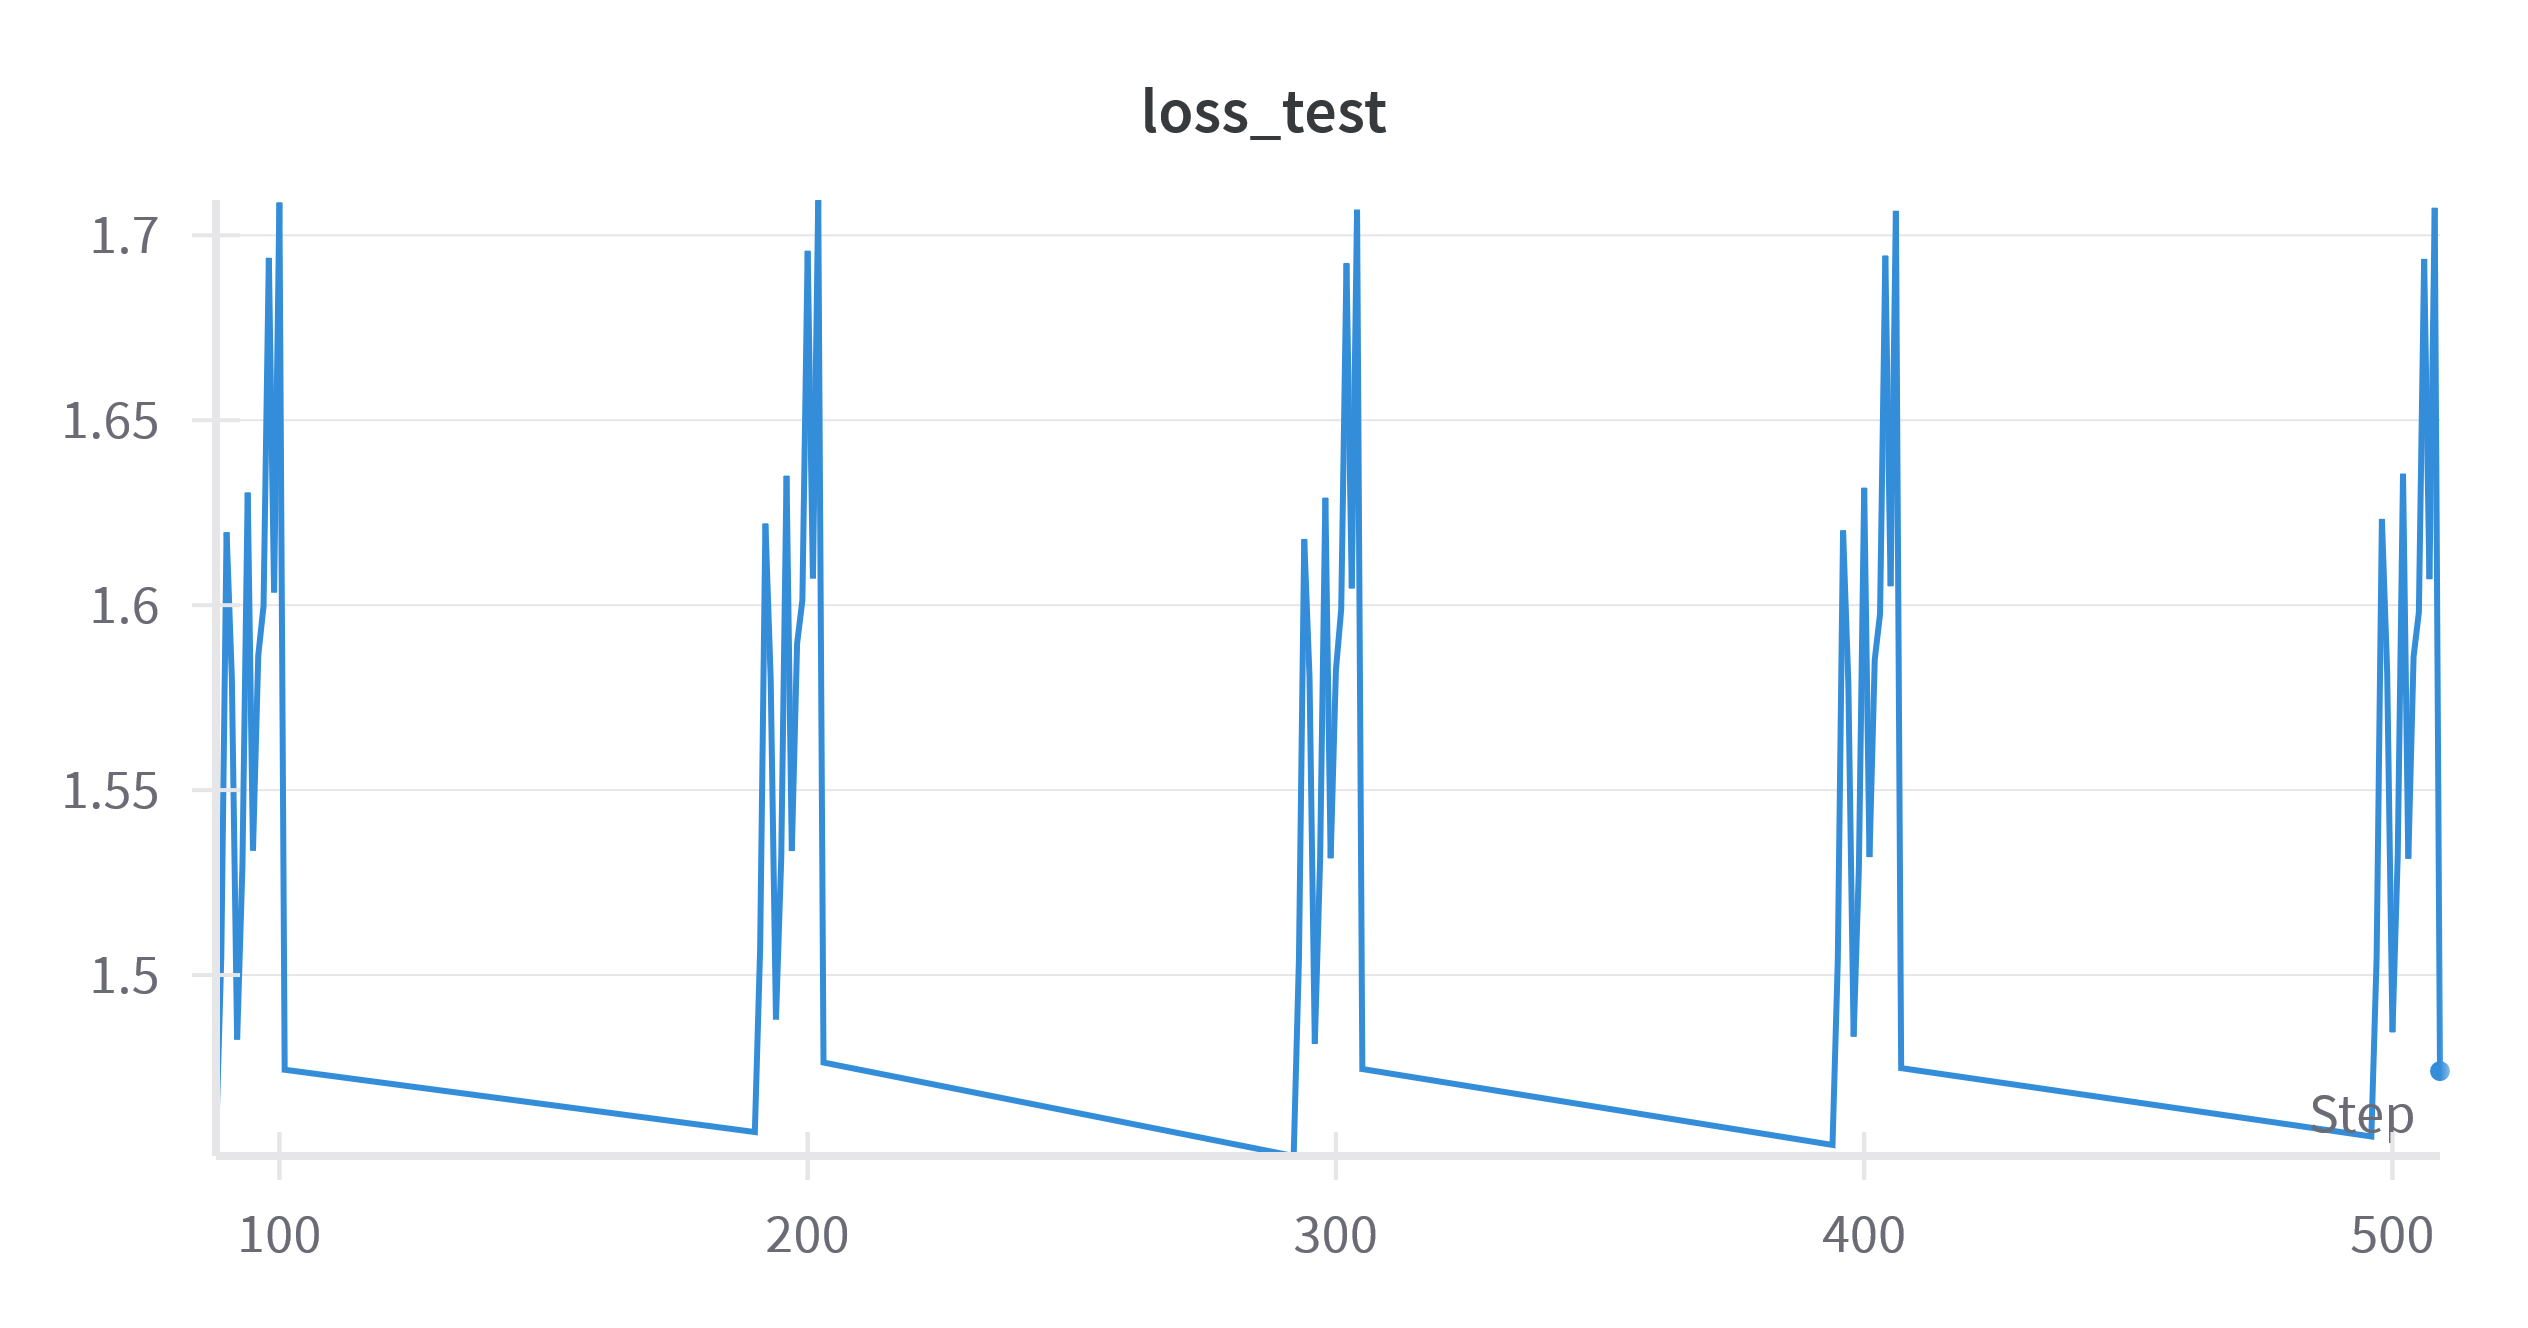
\includegraphics[width=0.45\linewidth]{figures/Figure33.png}}
    \label{fig:fig12}
    \caption{Loss graphs for the original EfficientDet D-0 model with pre-trained weights from the official GitHub account without anchors trained on train and then test sets for the first 10 epochs}
\end{figure}

\begin{figure}[H]
    \subfigure[Train loss]{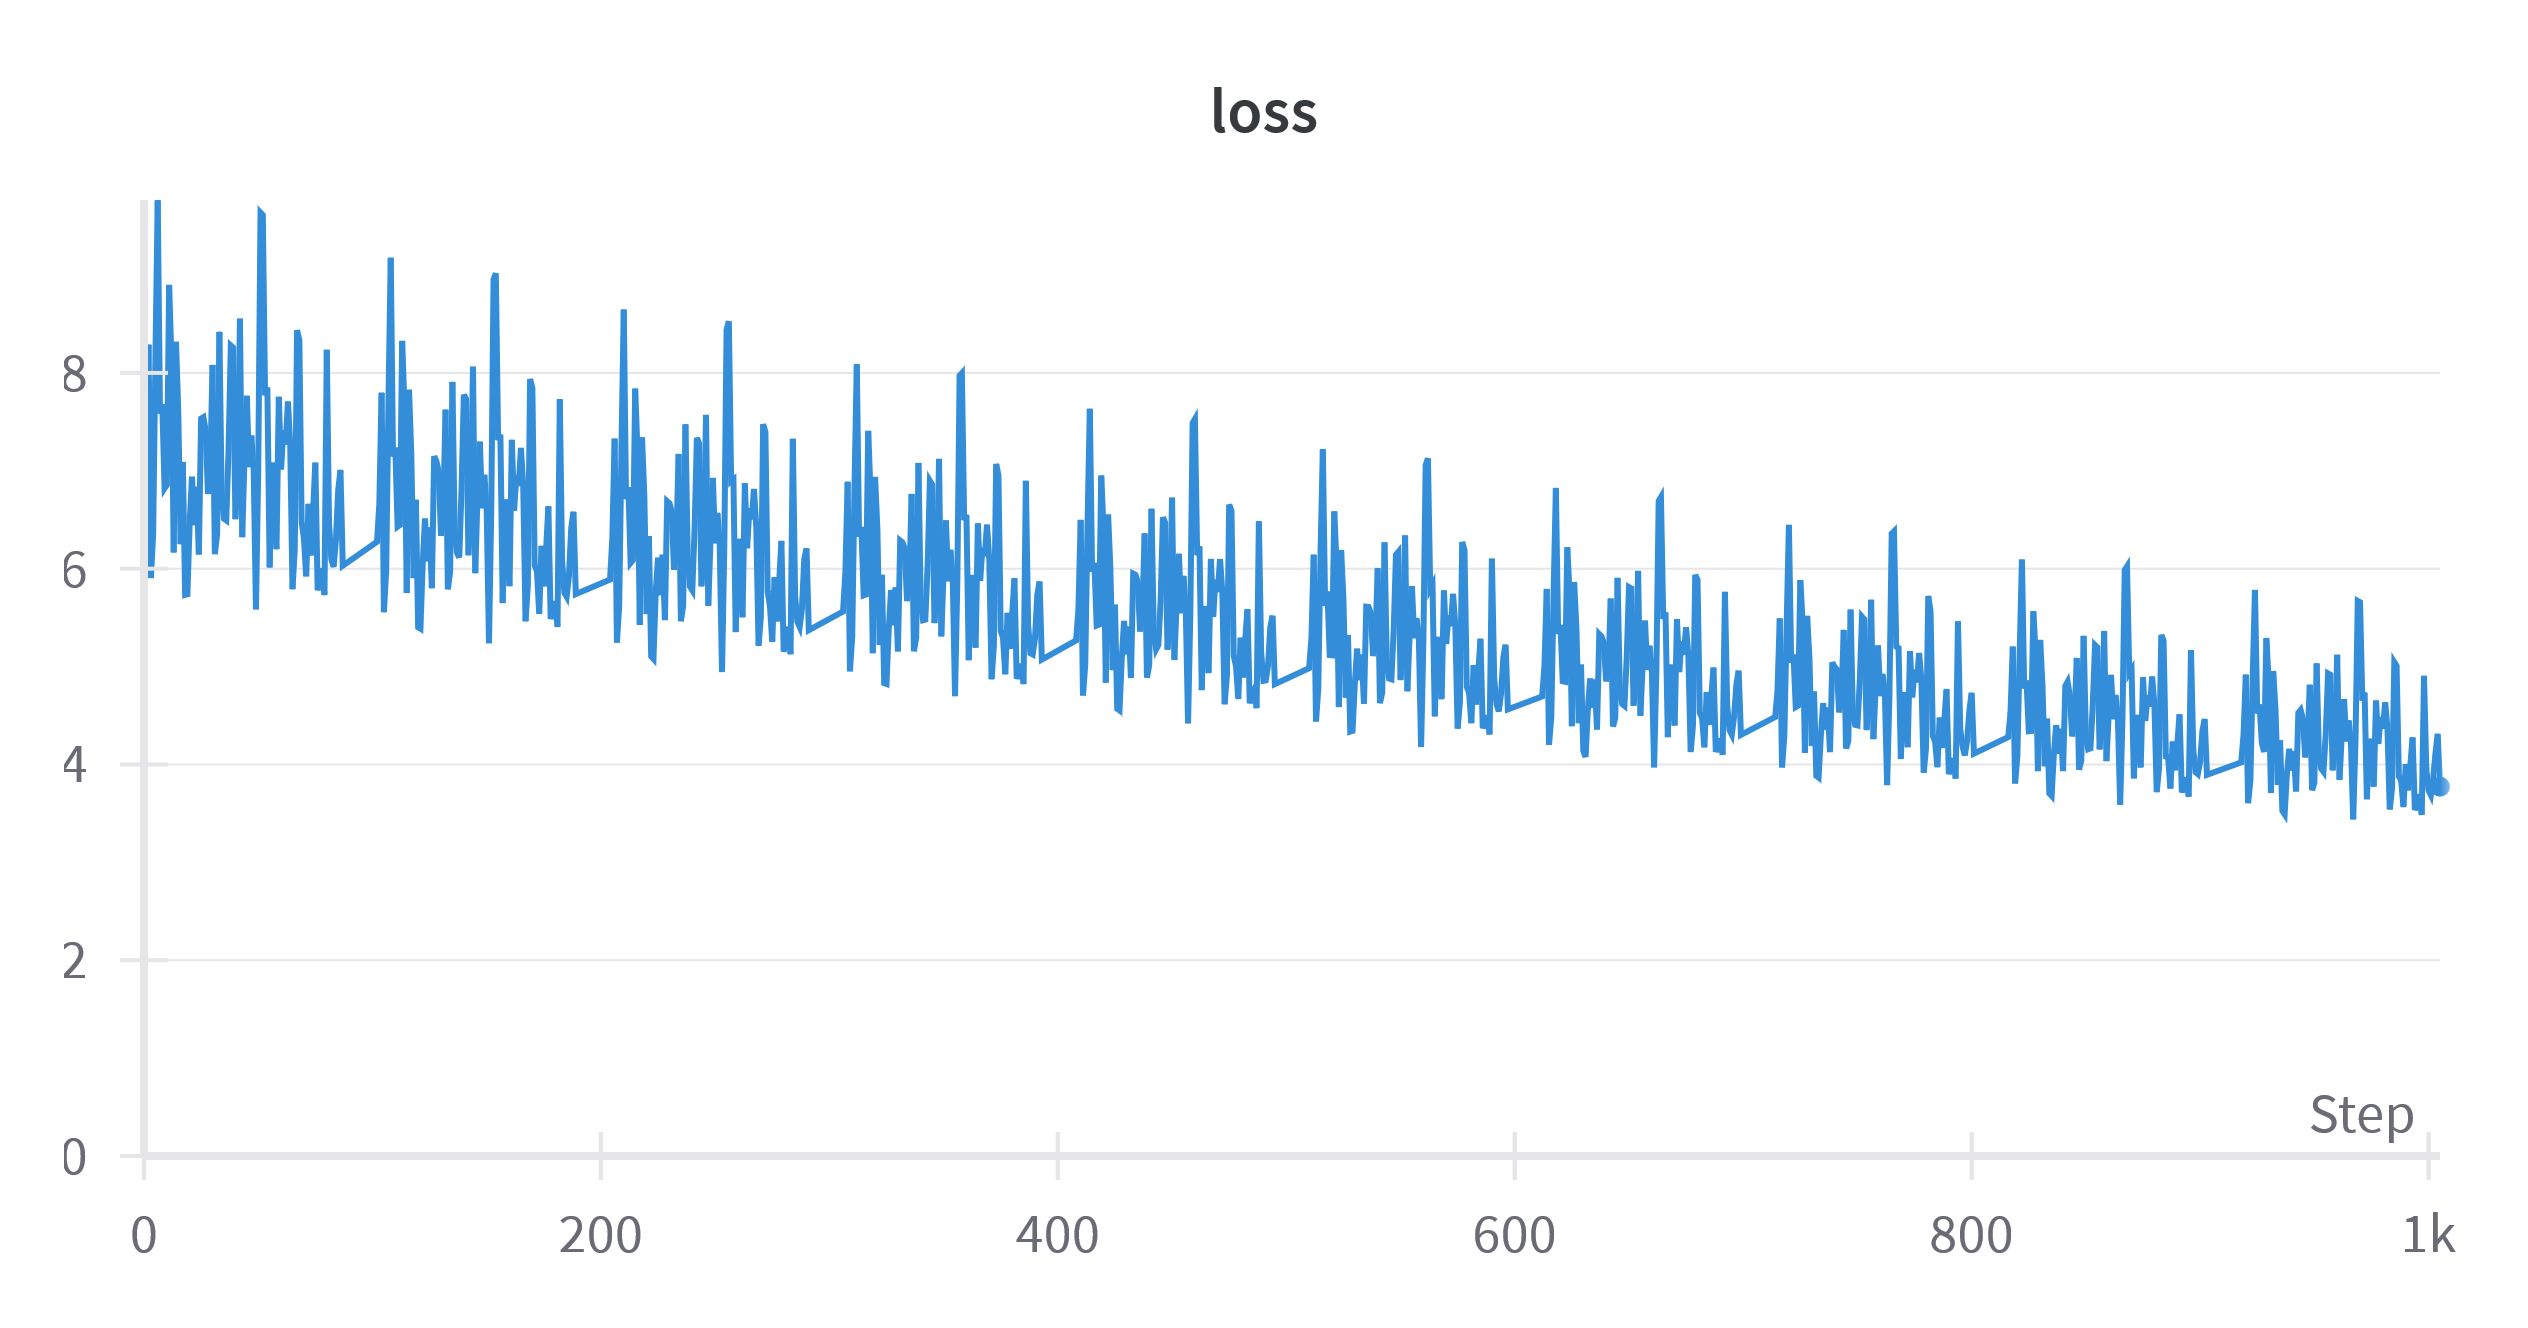
\includegraphics[width=0.45\linewidth]{figures/Figure41.png}}
    \subfigure[Test loss]{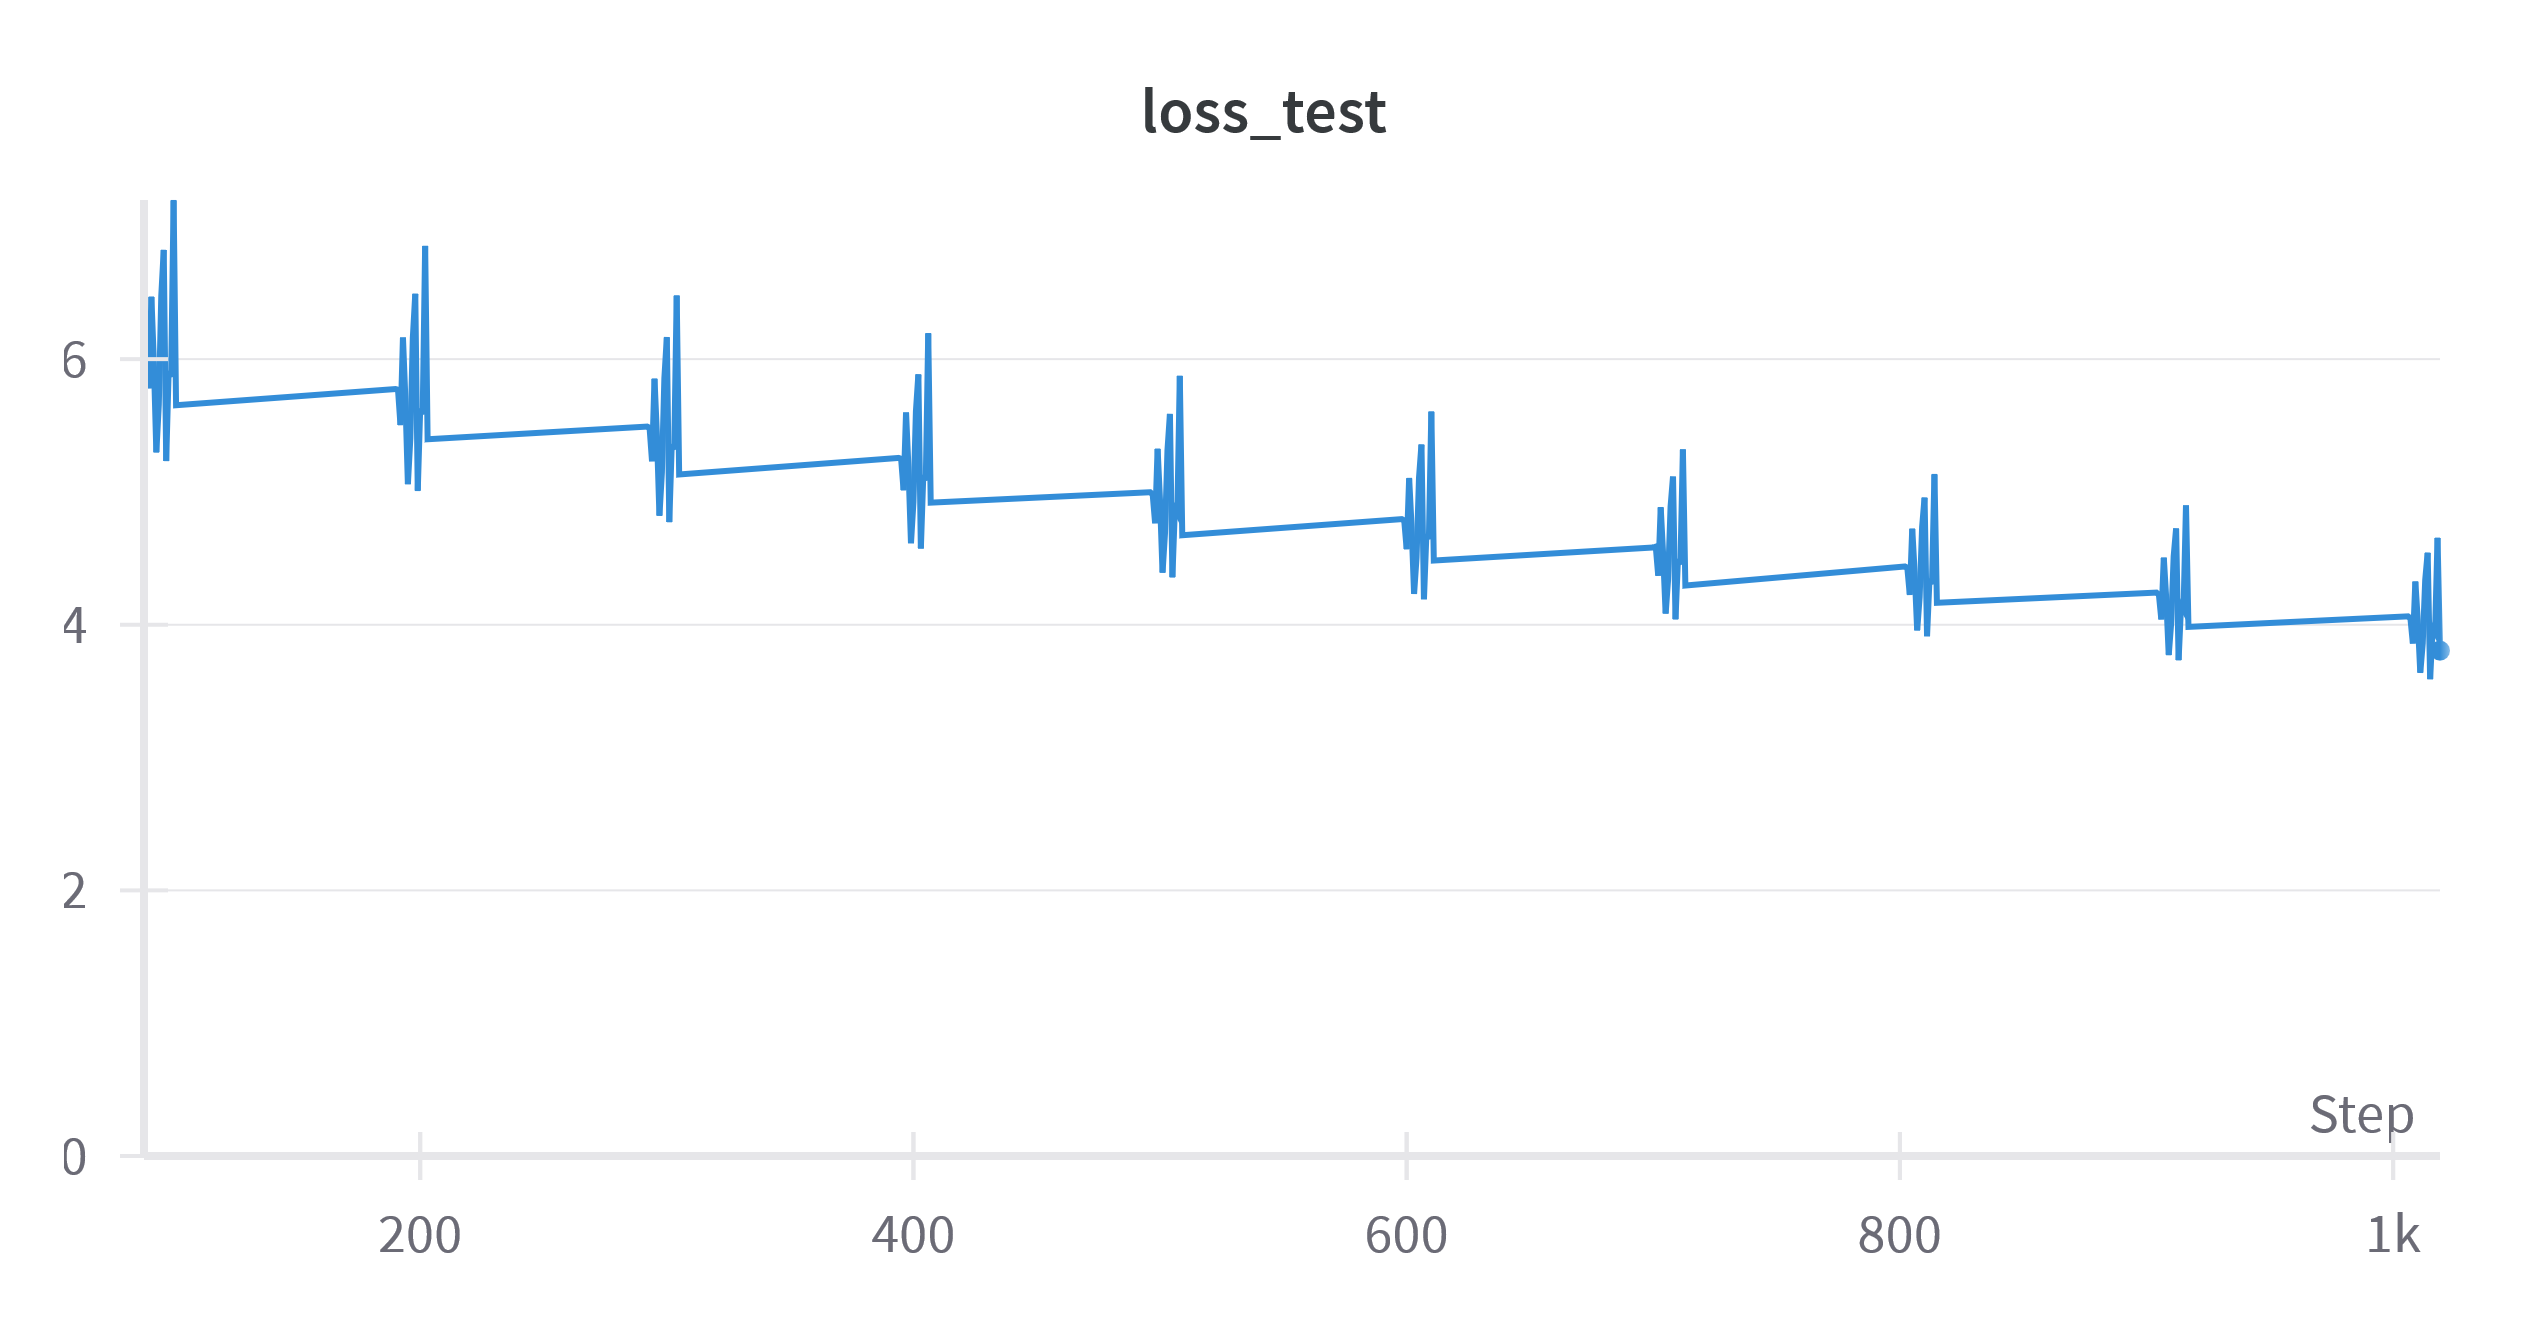
\includegraphics[width=0.45\linewidth]{figures/Figure42.png}}
    \label{fig:fig14}
    \caption{Loss graphs for the original EfficientDet D-0 model with pre-trained weights from the official GitHub account without anchors trained on train and then test sets for the 40 to 50 epochs}
\end{figure}

\subsection{Experiment 5}

For the next experiment, I wanted to see exactly how the model would operate after I called the initialization method. I again consulted the official implementation from GitHub ~\cite{link7} and discovered a key parameter, $bench\_labeler$ that I did not include in my call. This parameter, taking boolean values, True or False, was included in the initialization of the class DetBenchTrain if I chose to train the model rather than validate it. This goes on to be used in an if statement in the forward-pass method, and if this value proves to not be present in the call, it provides a warning before the code: \textit{target should contain pre-computed anchor labels if labeler not present in bench}. My pre-processing did not include any computation of anchor labels.

Anchors in the context of detection algorithms, also known as prior boxes, are bounding boxes computed before the actual training that help the model better understand what size the objects in the images would be. For example, if the model was intended to recognize people from an image, the anchor boxes might be chosen to be taller rather than wider so as to match the aspect ratio of the shape of a person.~\cite{link11}

The basic configuration that the Effdet library has to offer does include some anchor labels, based on the overall size of the images, so I chose to use those and see how the predictions would turn out. The way the model was initialized is this: $create\_model\_from\_config(config=config, bench\_task='train', num\_classes=2, pretrained=True, bench\_labeler = True)$.

This proved to be a very good discovery. The hyper-parameters were the same as in the previous experiment. I only ran one epoch of this configuration, so there is no test loss. Figure \ref{fig:fig34} shows how the train loss looked for the first epoch.

\begin{figure}[H]
    \centering
    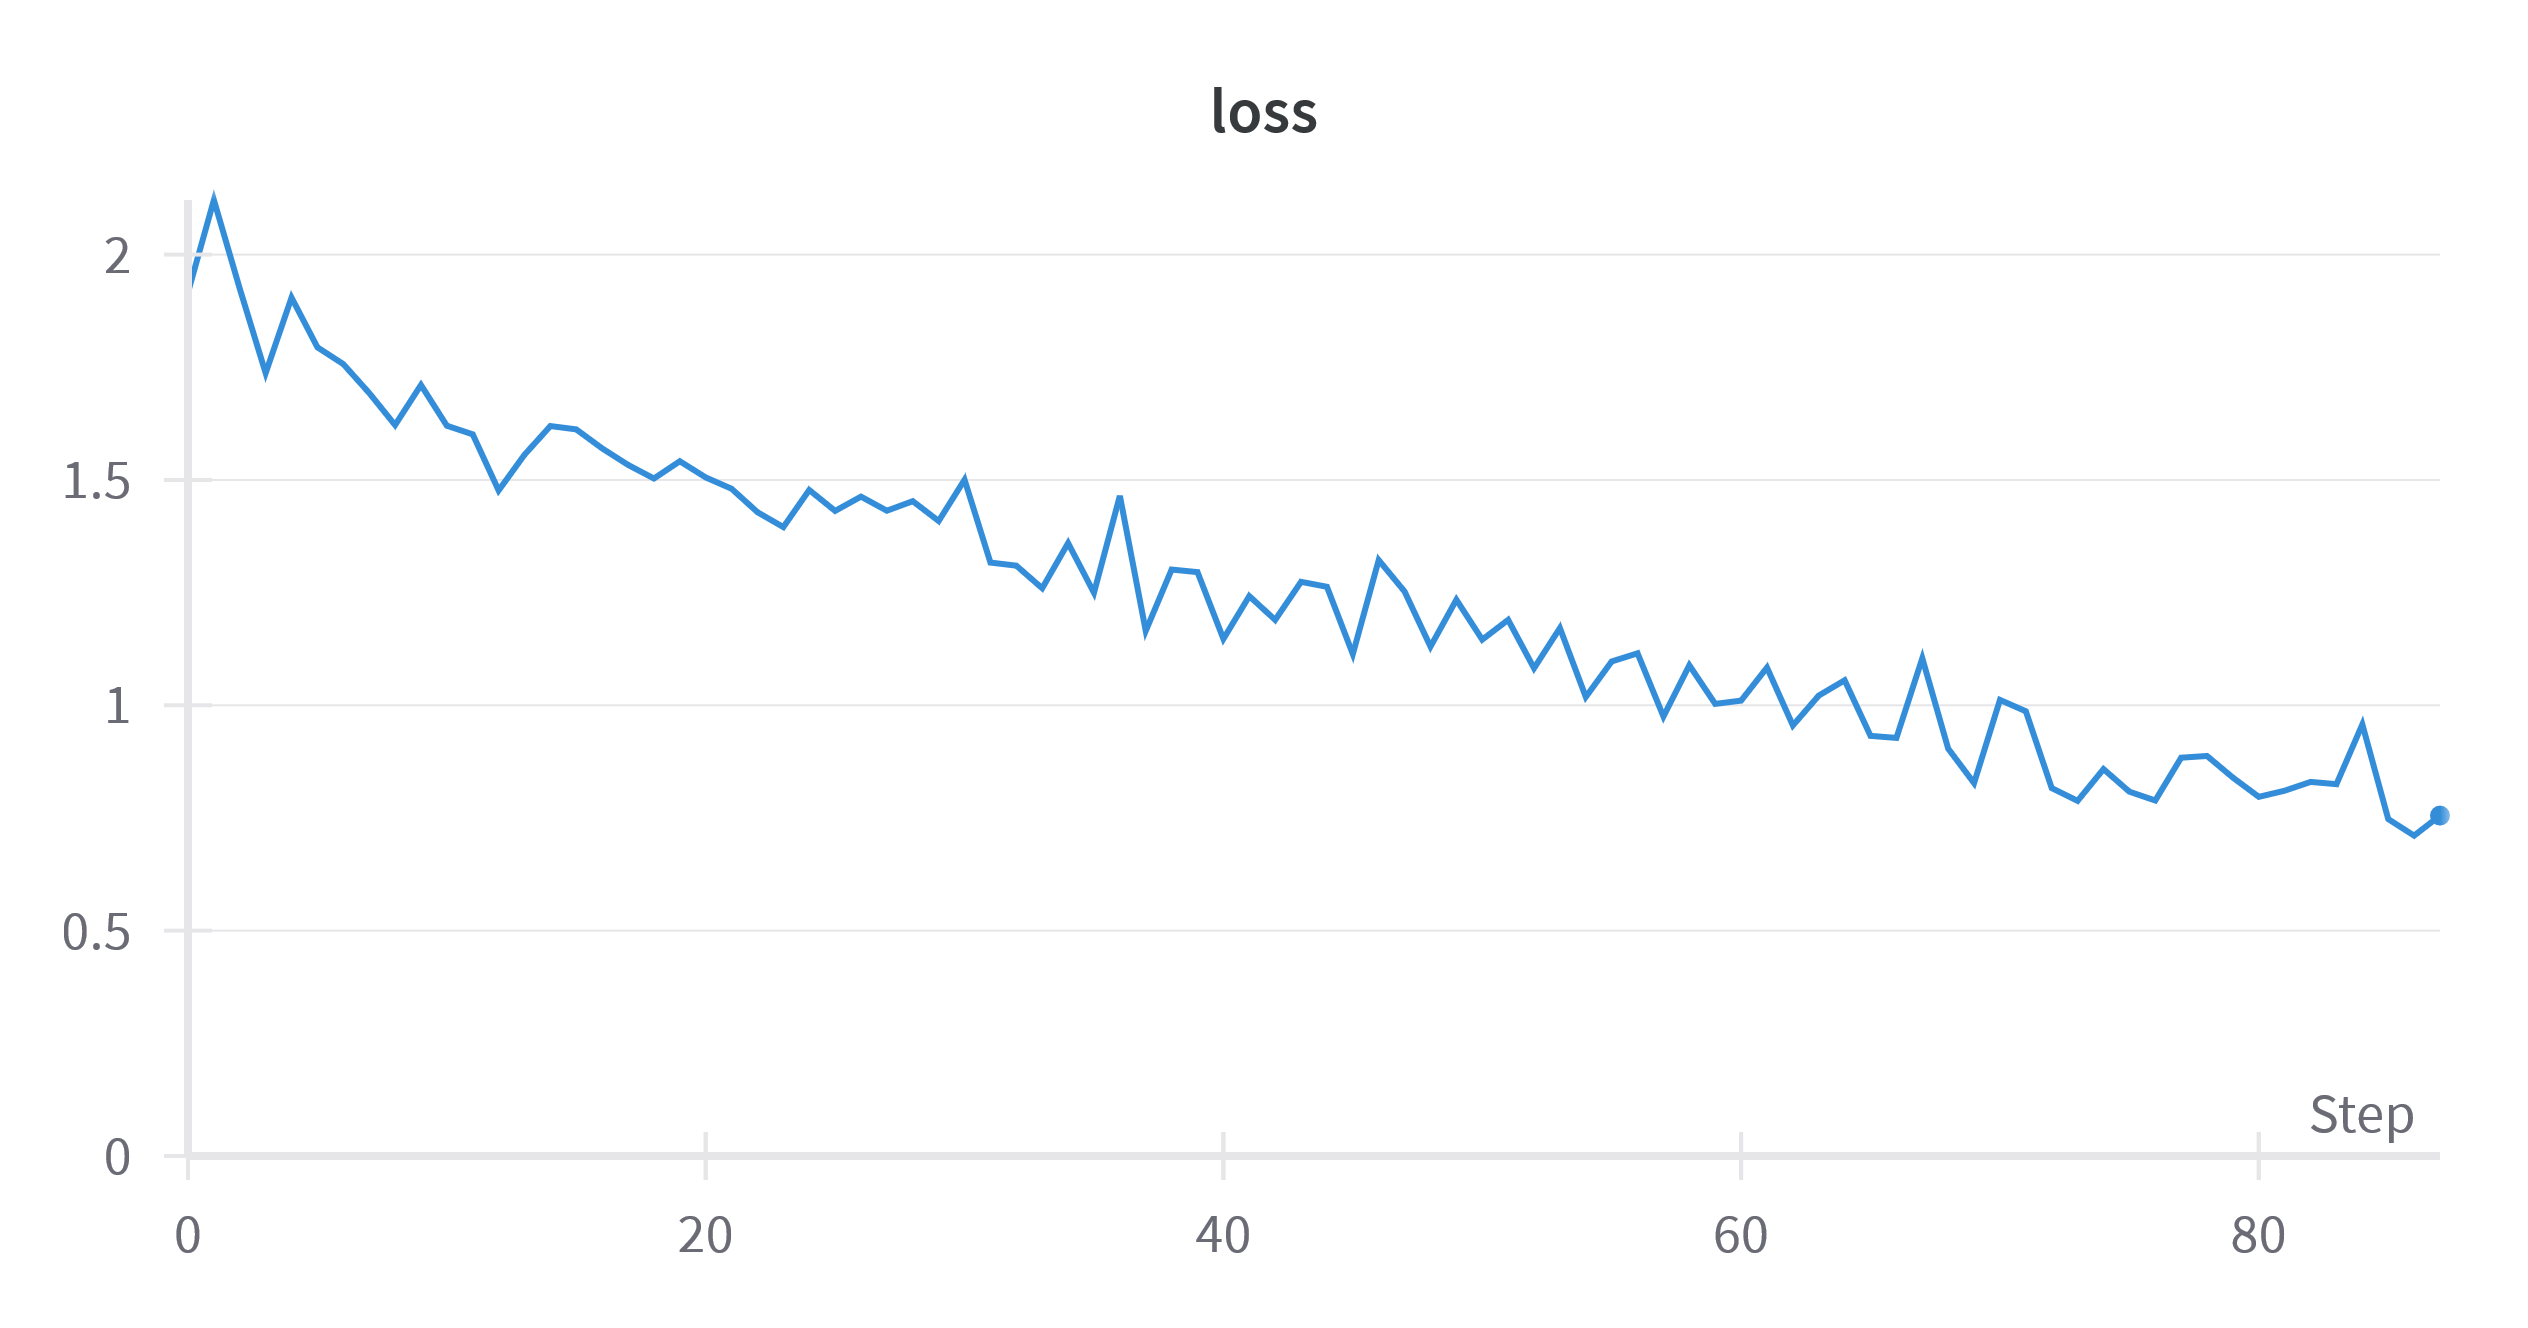
\includegraphics[width=0.5\linewidth]{figures/Figure43.png}
    \caption{Loss graphs for the original EfficientDet D-0 model with pre-trained weights from the official GitHub account with anchors trained on the train set for one epoch}
    \label{fig:fig34}
\end{figure}

This is the first experiment where the initial loss is ideal. Keeping this in mind, I kept almost the same configuration for the next experiment, besides training the model for more epochs.

\subsection{Experiment 6}

The learning rate decay in experiment 5 was used after each step, meaning each batch, in the train dataset, and also at the end of all of the batches. In this experiment, I stopped calling the step function after all the batches and kept it after each batch. Figure \ref{fig:fig35} shows how the train and test losses looked for the 10 epochs that the model has been trained for.

\begin{figure}[ht]
    \subfigure[Train loss]{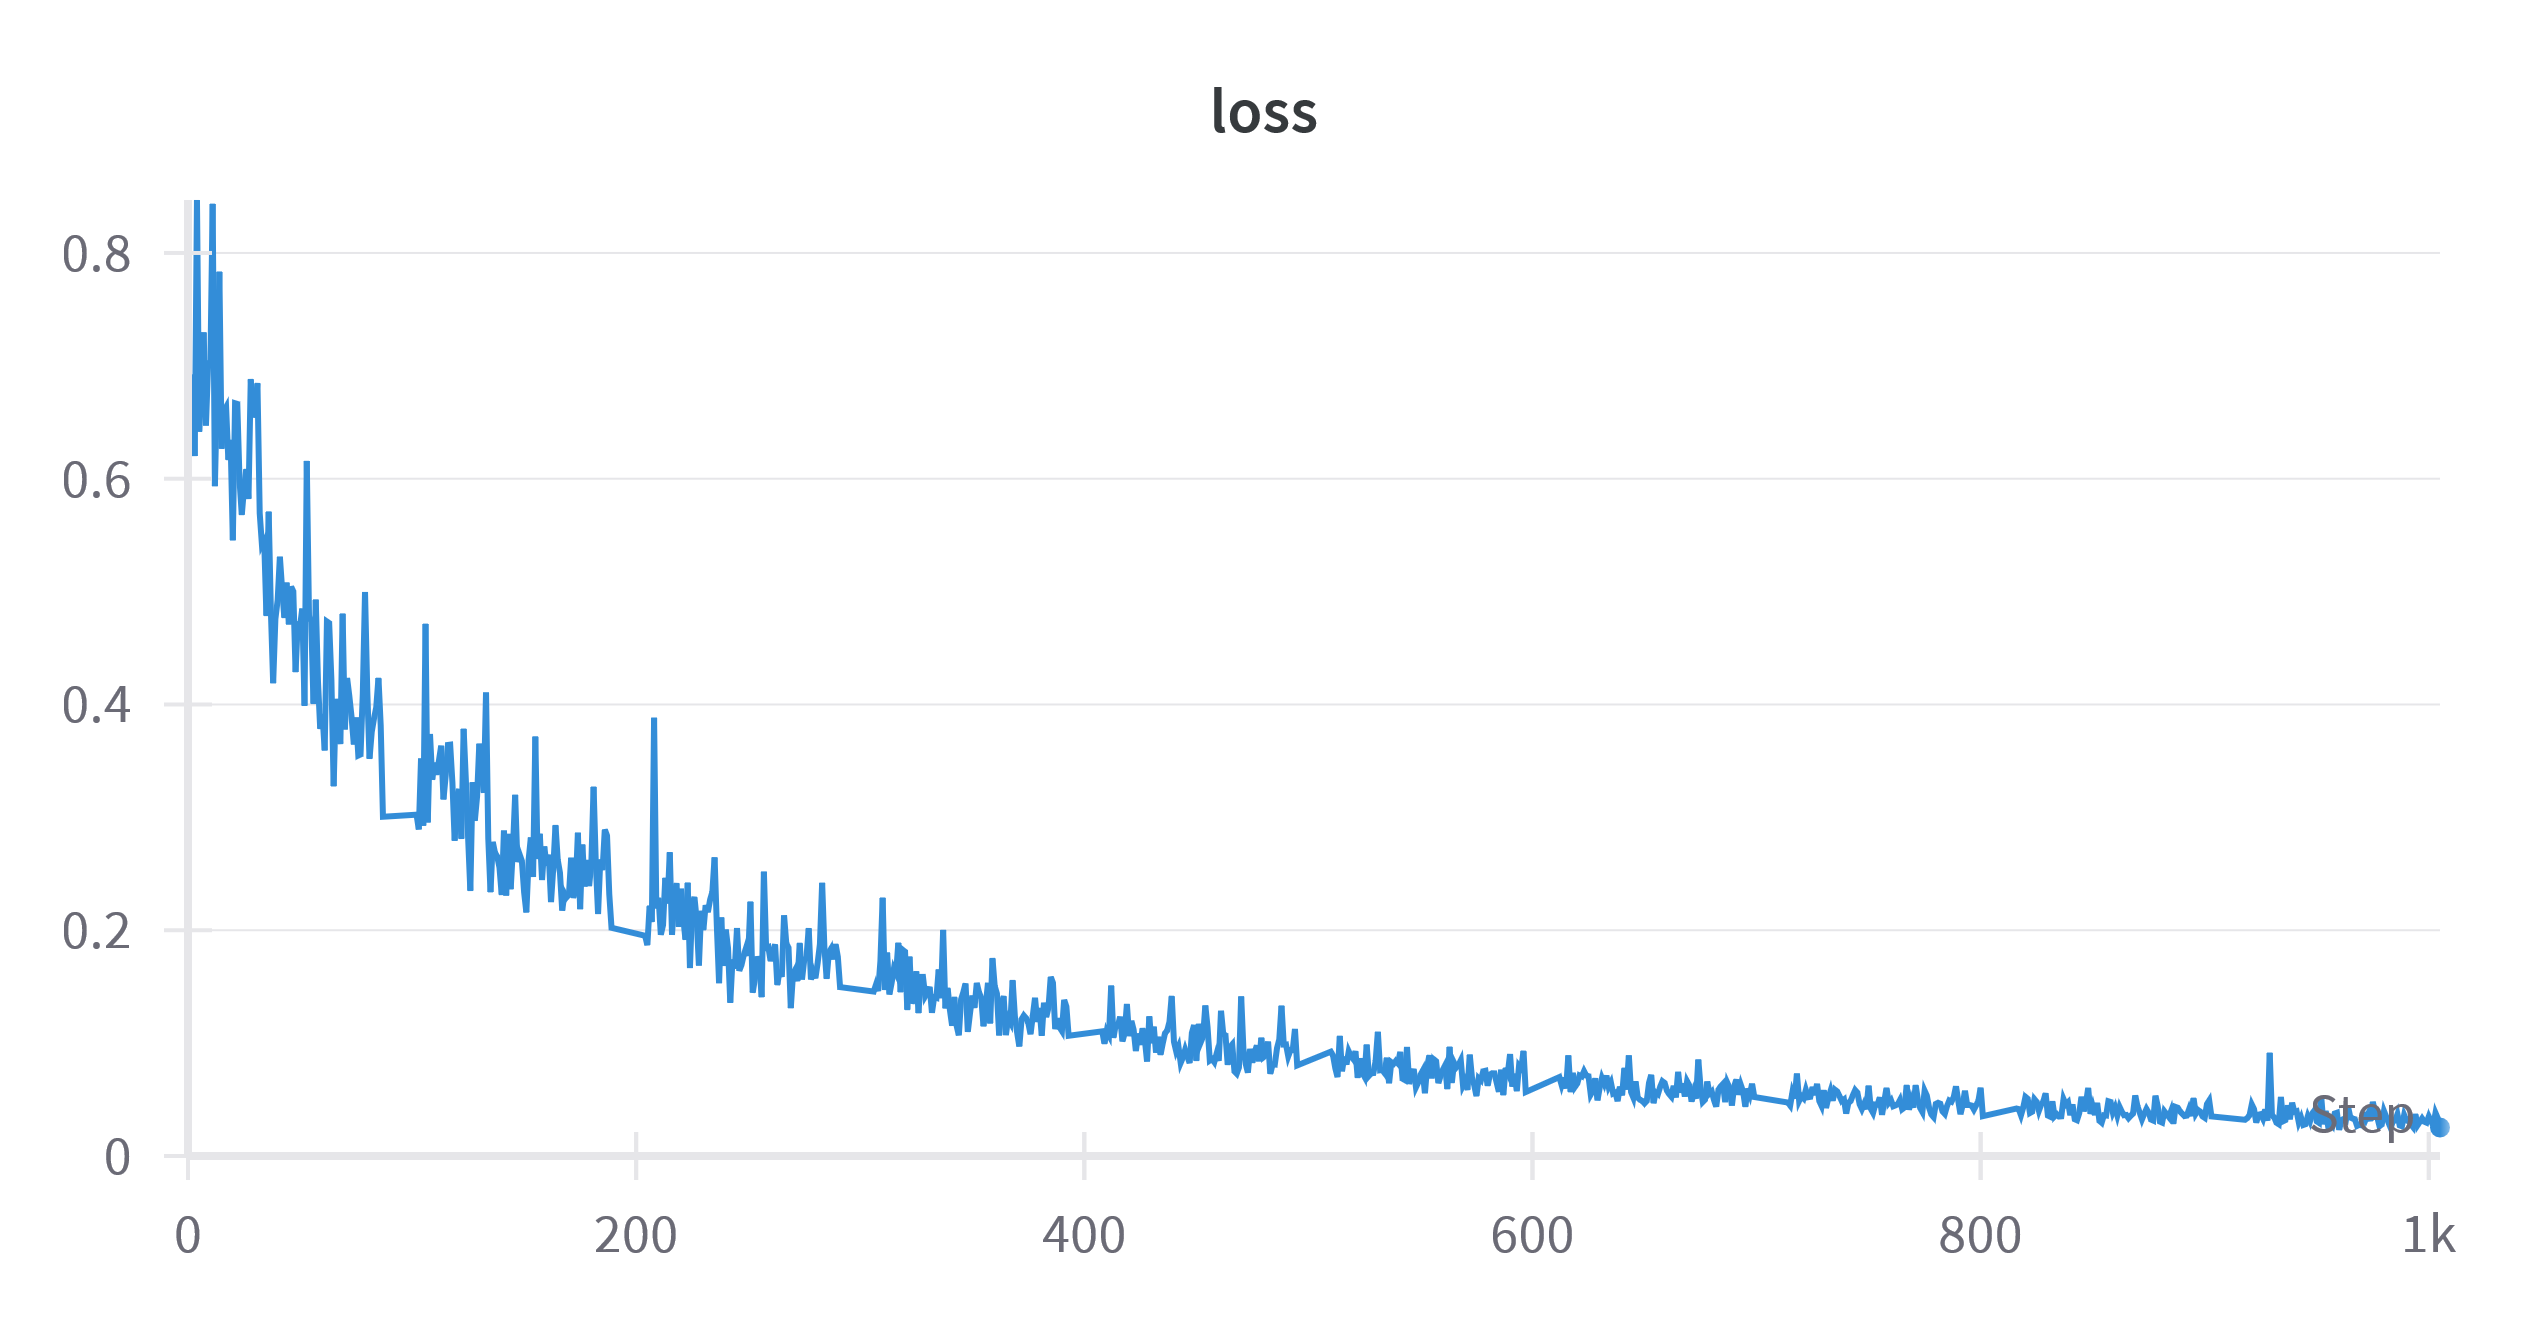
\includegraphics[width=0.45\linewidth]{figures/Figure44.png}}
    \subfigure[Test loss]{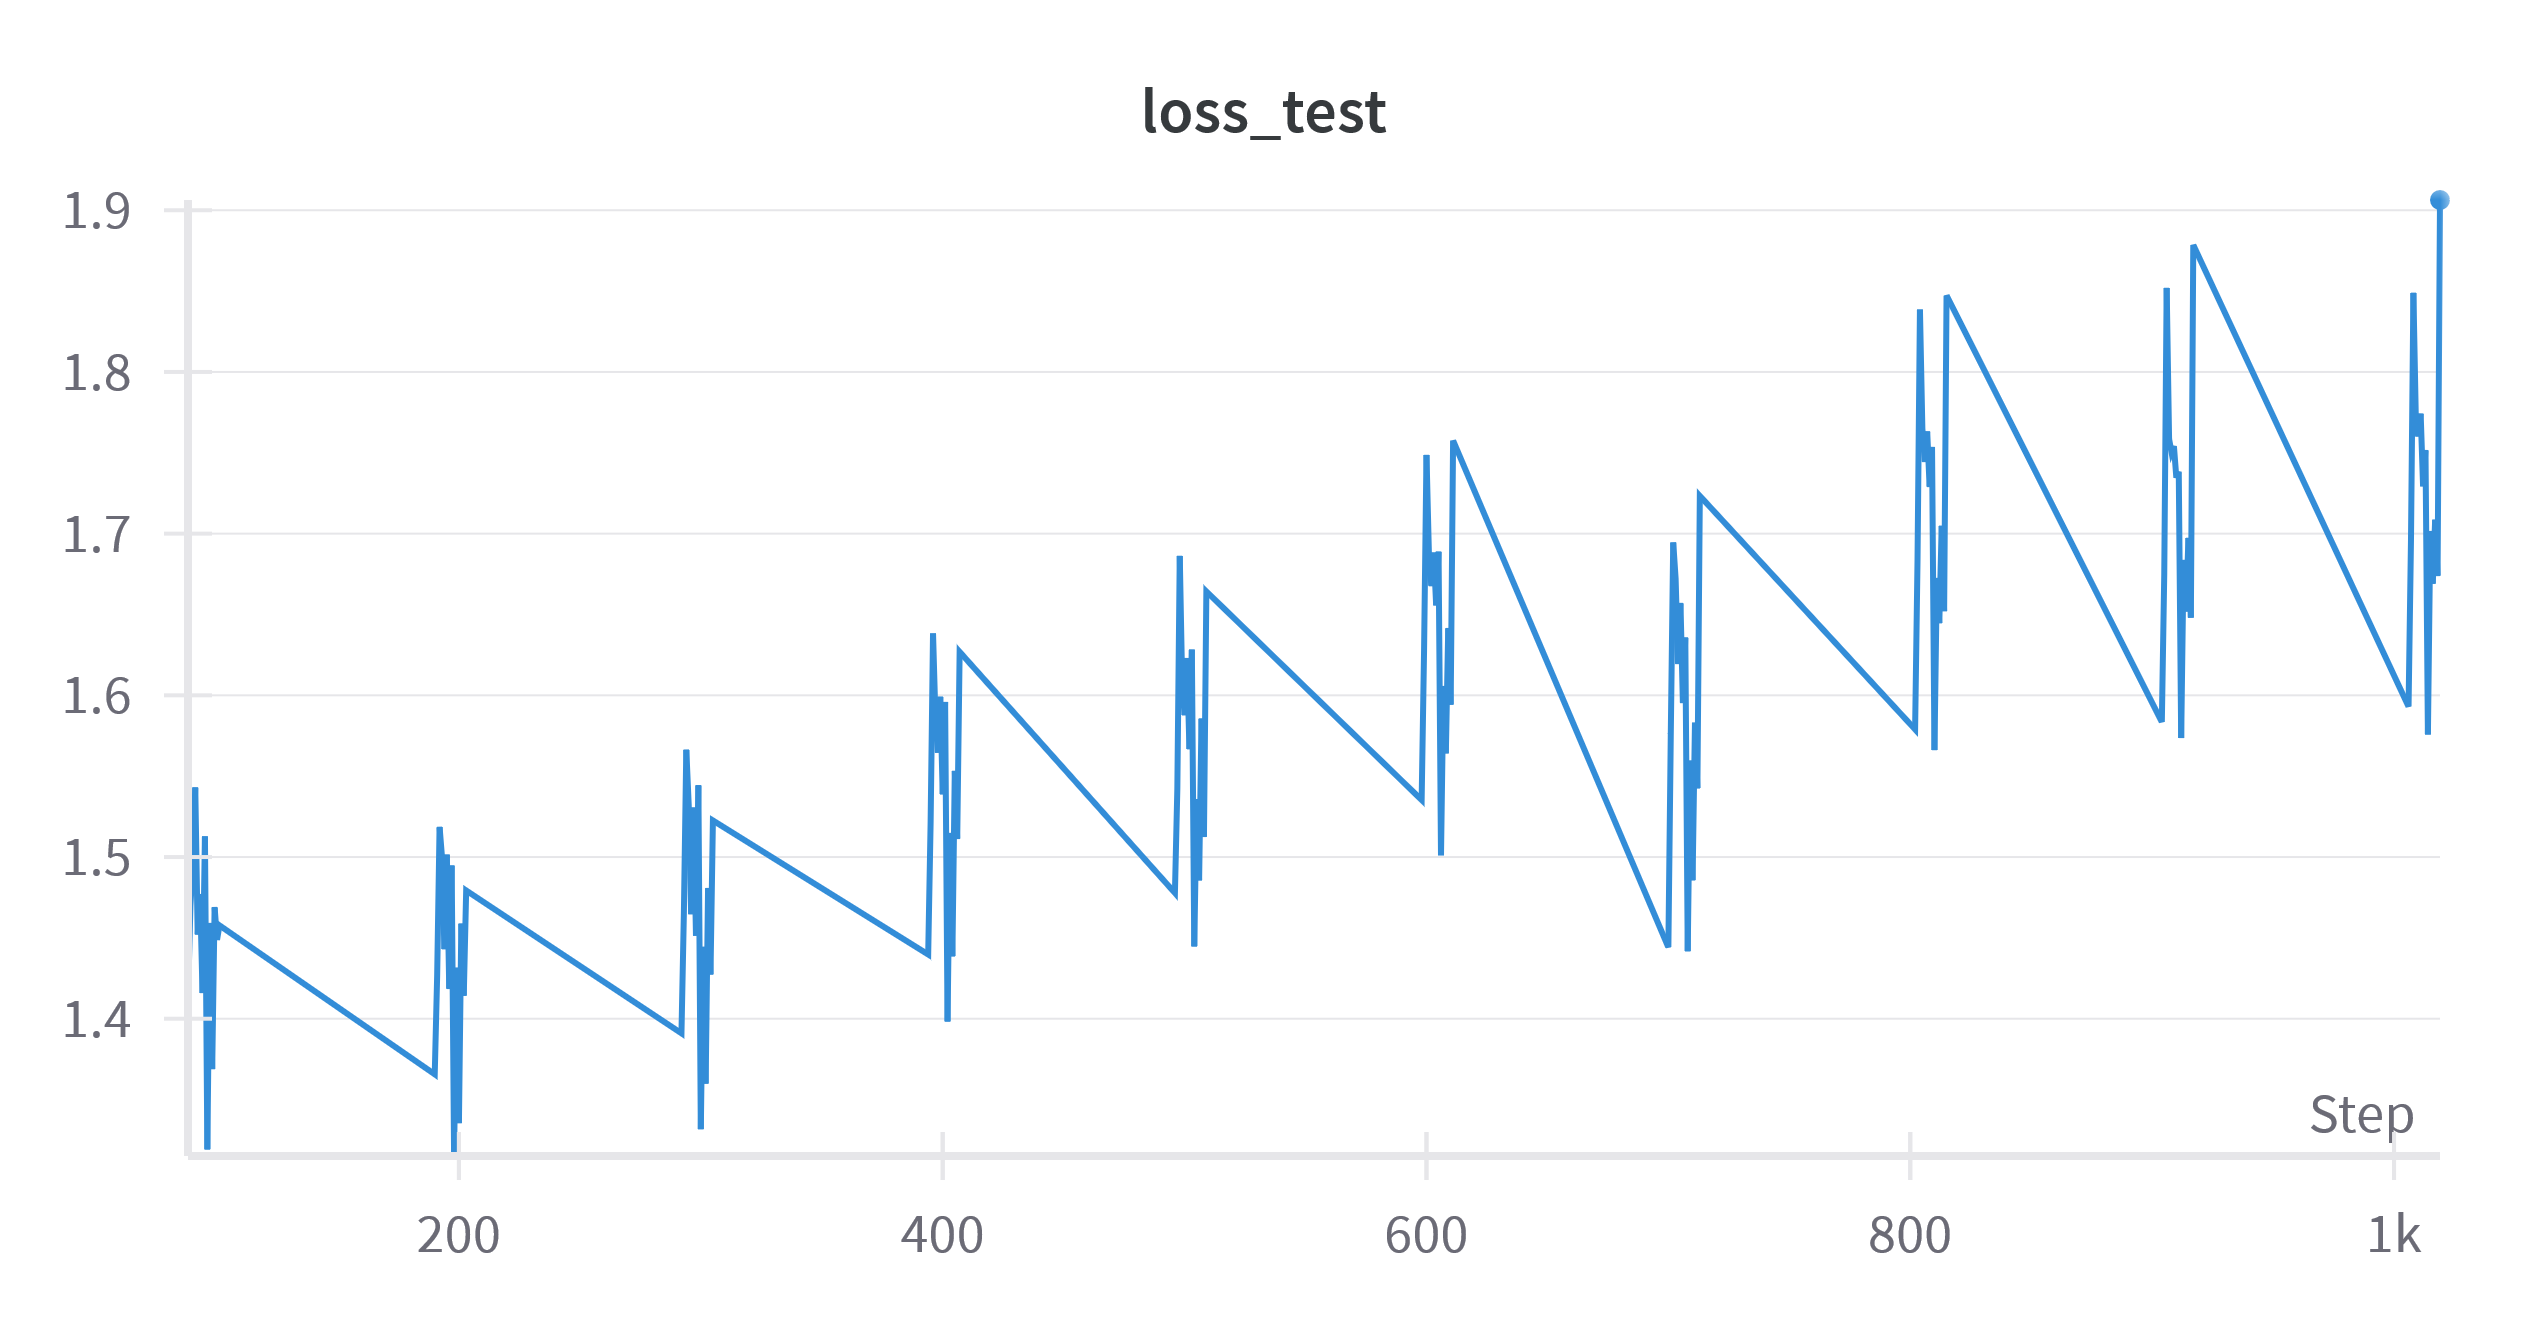
\includegraphics[width=0.45\linewidth]{figures/Figure45.png}}
    \label{fig:fig35}
    \caption{Loss graphs for the original EfficientDet D-0 model with pre-trained weights from the official GitHub account with anchors trained on train and then test sets for 10 epochs}
\end{figure}

The image \ref{fig:fig36} shows real bounding boxes drawn on the picture they belong to versus predicted bounding boxes drawn on the same pictures.

\begin{figure}[ht]
    \subfigure[Train predictions]{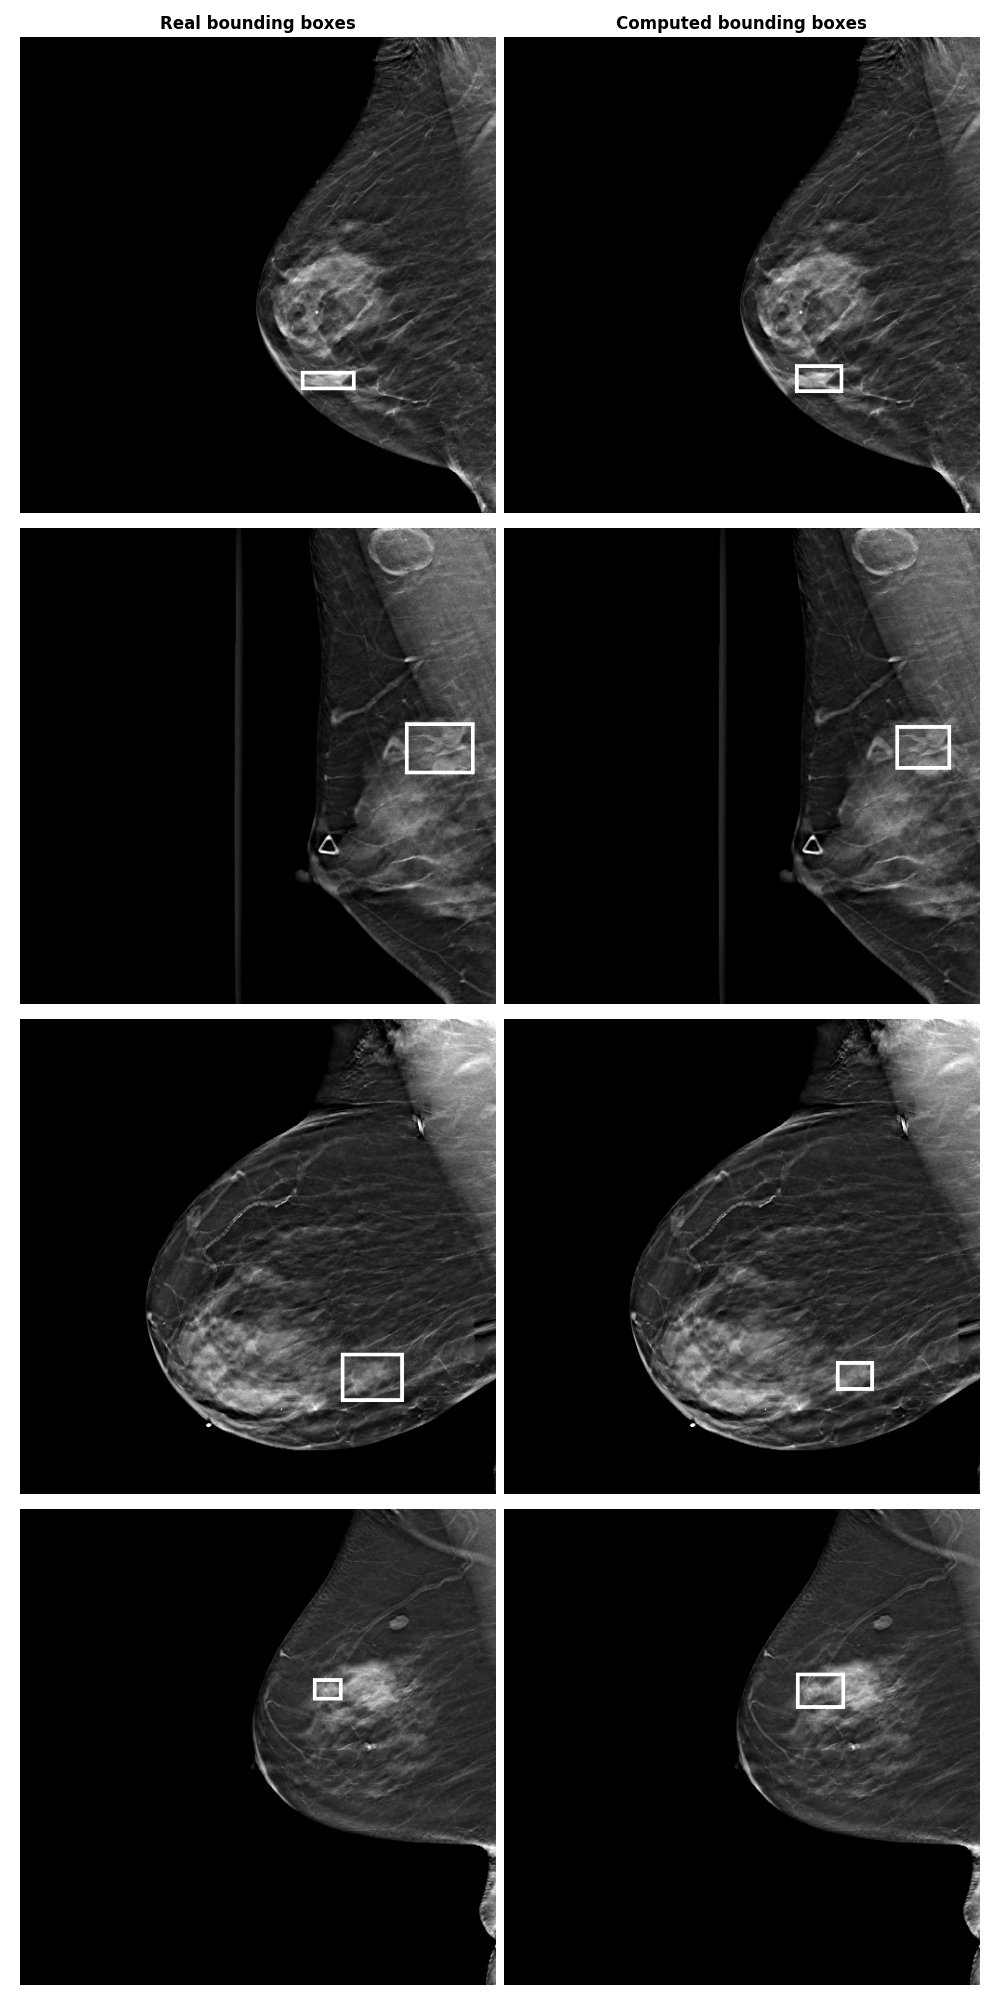
\includegraphics[width=0.45\linewidth]{figures/Figure47.png}}
    \subfigure[Test predictions]{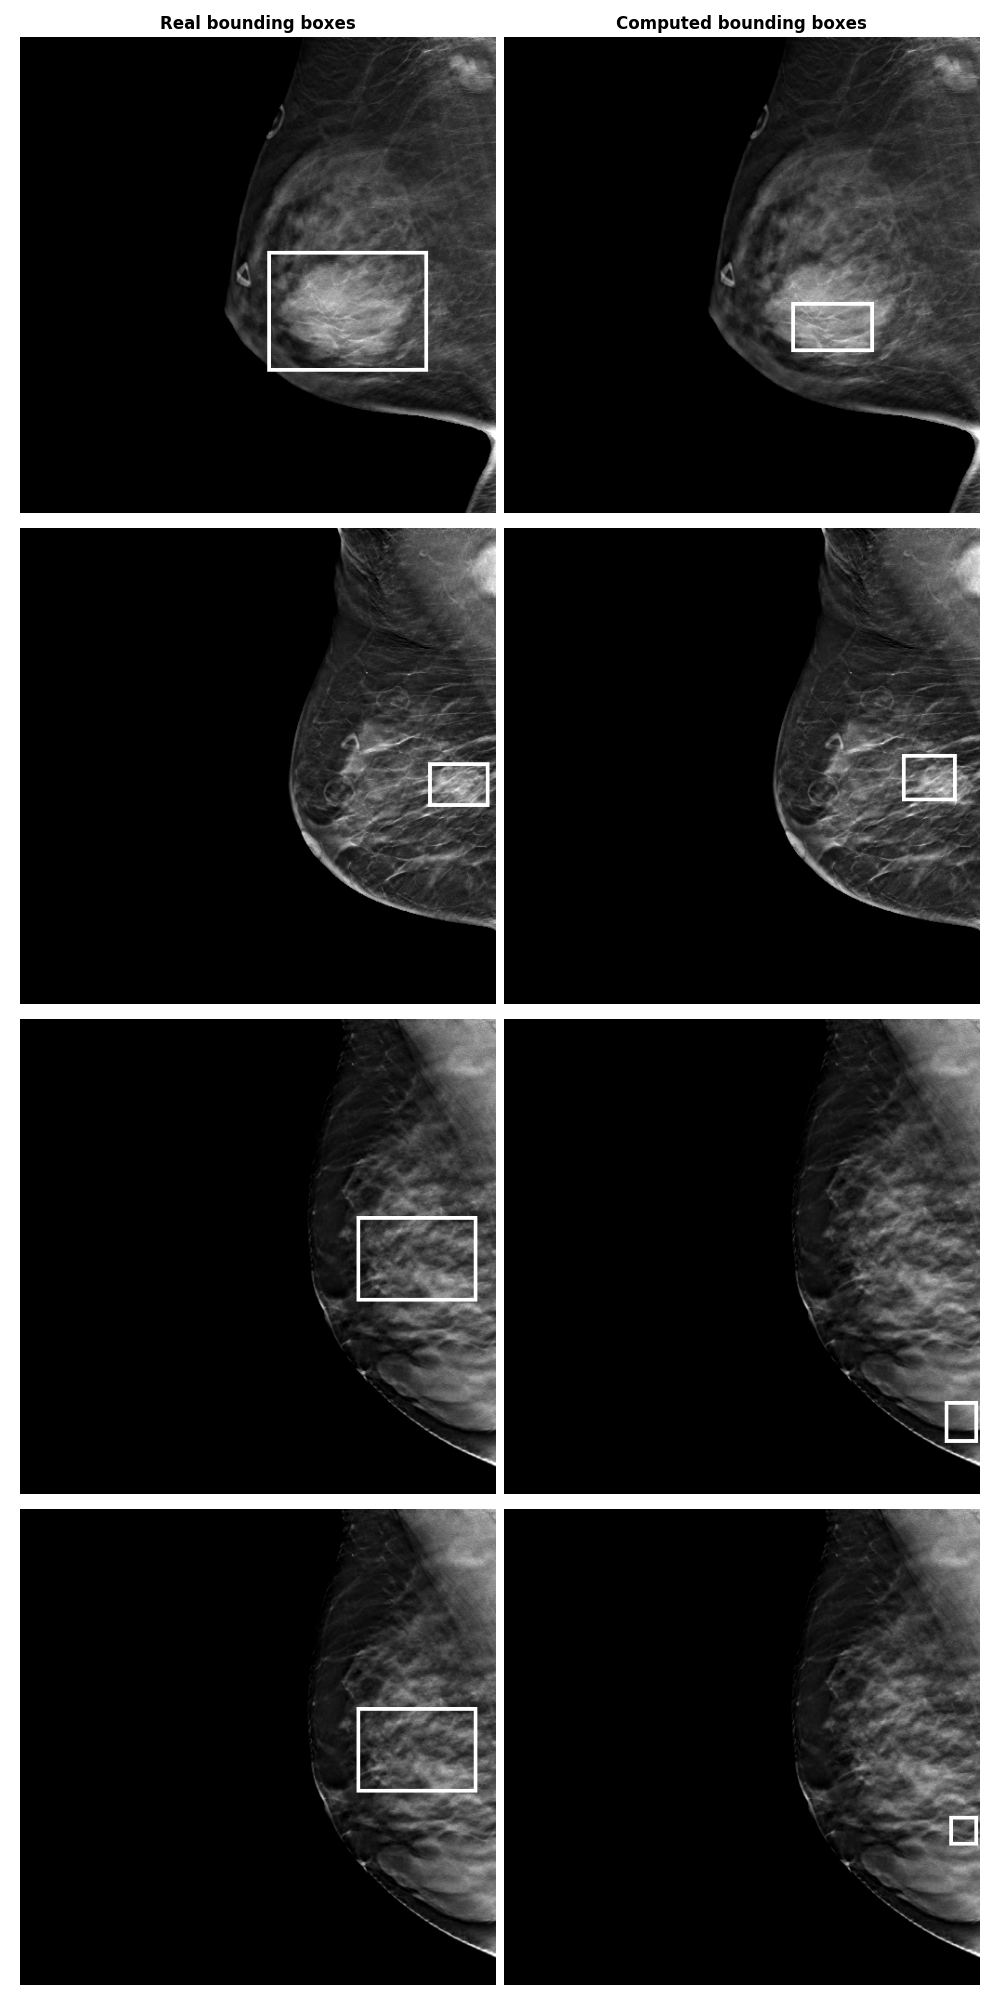
\includegraphics[width=0.45\linewidth]{figures/Figure46.png}}
    \label{fig:fig36}
    \caption{List of predictions vs. real  bounding boxes on the train and test set}
\end{figure}

As it appears the test loss increases with each epoch, I chose to integrate into the system the model after 2 epochs. Therefore, the final configuration for the detection model is: batch size of 16, image size of 3$\times$512$\times$512, the images were normalized, learning rate of 0.0001 with a CosineAnnealing learning rate decay applied after each batch in the training loop and an Adam optimizer.

Tables \ref{tab:tab8}, \ref{tab:tab9} and \ref{tab:tab10} show the conclusions of these experiments.

\begin{table}[!ht]
    \centering
    \begin{tabular}{|c|c|c|c|c|}
       \hline
       Experiment  & Image size & Model & trained/pre-trained\\
       \hline\hline
       Exp1 & 3$\times$512$\times$512 & EfficientDet & trained\\
       \hline
       Exp2 & 3$\times$512$\times$512 & EfficientDet without anchors & pre-trained from Kaggle\\
       \hline
       Exp3 & 3$\times$512$\times$512 & EfficientDet without anchors & pre-trained from GitHub \\
       \hline
       Exp4 & 3$\times$512$\times$512 & EfficientDet without anchors & pre-trained from GitHub \\
       \hline
       Exp5 & 3$\times$512$\times$512 & EfficientDet with anchors & pre-trained from GitHub \\
       \hline 
       Exp6 & 3$\times$512$\times$512 & EfficientDet with anchors & pre-trained from GitHub \\
       \hline
    \end{tabular}
    \caption{Detection models}
    \label{tab:tab8}
\end{table}

\begin{table}[H]
    \centering
    \begin{tabular}{|c|c|c|c|c|}
       \hline
       \multirow{3}{5em}{Experiment}  & \multicolumn{4}{c|}{Performance}
       \\ \cline{2-5}
        & \multicolumn{2}{c|}{Test loss} & \multicolumn{2}{c|}{Train loss}
        \\ \cline{2-5}
        & Maximum & Minimum & Maximum & Minimum \\
       \hline \hline
       Exp1 & 9146.229 & 402.704 & 1411.082 & 543.197 \\ \hline
       Exp2 & 795.51 & 1.473 & 1471.658 & 0.622 \\ \hline
       Exp3 & 1.712 & 1.451 & 0.9926 & 0.5174 \\ \hline
       Exp4 & 33736.91 & 3.589 & 53161.637 & 3.437\\ \hline
       Exp5 & & & 2.121 & 0.7108 \\ \hline
       Exp6 & 1.906 & 1.315 & 0.8469 & 0.02313\\ \hline

    \end{tabular}
    \caption{Detection models(continuation)}
    \label{tab:tab9}
\end{table}

\begin{table}[H]
    \centering
    \begin{tabular}{|c|c|c|c|c|}
       \hline
       \multirow{2}{5em}{Experiment}  & \multicolumn{4}{c|}{Hyper parameters} \\ \cline{2-5}
       % \hline
        & learning rate & learning rate decay & minimum lr &  step method called\\
       \hline \hline
       Exp1 & 0.0001 & ReduceLROnPlateau & $1e^{-8}$ & after test loop \\
       \hline
       Exp2 & 0.0001 & ReduceLROnPlateau & $1e^{-8}$ & after test loop \\
       \hline
       Exp3 & 0.0001 & ReduceLROnPlateau & $1e^{-8}$ & after test loop \\
       \hline
       \multirow{2}{*}{Exp4} & \multirow{2}{*}{0.0001} & \multirow{2}{*}{CosineAnnealingLR} & \multirow{2}{*}{$1e^{-6}$} & after each batch\\
       & & & & after train loop \\
       \hline
       \multirow{2}{*}{Exp5} & \multirow{2}{*}{0.0001} & \multirow{2}{*}{CosineAnnealingLR} & \multirow{2}{*}{$1e^{-6}$} & after each batch\\
       & & & & after train loop \\
       \hline 
       Exp6 & 0.0001 & CosineAnnealingLR & $1e^{-6}$ & after each batch\\
       \hline
    \end{tabular}
    \caption{Detection models(continuation)}
    \label{tab:tab10}
\end{table}

\chapter{"Deep Learning Techniques for Breast Cancer Detection: A Comparative Study of GoogLeNet and EfficientDet in 3D Imaging" System Interface}
\label{chap:ch5}
\section{Functionalities}
The system consists of two main functionalities: selecting an image, either from the array of examples provided in the top right corner of the interface, or the upload button which opens the computer's internal storage. Upon selecting an image, it will be viewed in the main window. The image selected does not necessarily have to be 512$\times$512, because it will be resized anyway. The user then has the choice of either selecting another image or submitting the image to the model to be classified into normal and cancerous, the latter being then sent to the detection model to replace the image in the main window with the same image that has drawn the bounding box resulted from passing the image to the model. 

The detection model also classifies the tumors into benign or malign. In the bottom right corner, below the examples image array, there 2 boxes. The top one contains the top two classes the models classified the image as while the bottom one displays the true label of the image, if it was selected from the examples array. If the image has not been selected from the examples array, the bottom box will contain the word "unknown".

Because the way this library sends the data from the image selected doesn't include the actual name of the filename, I found myself thinking of ways to find and display the true label of the images selected from the examples. To do so, I compared the contents of each of the images existing in the directory to the contents of the image selected. In preparation for this, for each image saved as index.png, index being a variable from 1 to 151, I saved an additional file named index-label.txt, where label is either 0 or 1, corresponding to the labels normal or cancer. For the images uploaded from the user's device, there is no way to find the true label of the input, therefore, I added another class, unknown, that is displayed whenever the label of the image cannot be determined.

Comparatively, if the image is detected to be normal, the main window will not change, instead displaying the original image.

\section{Design}

Figure \ref{fig:fig38} shows the architecture diagram. Figure \ref{fig:fig39} shows the class diagram. The Fitter class is used to train the detection model, the classification model is trained in a simple loop. Figure \ref{fig:fig40} shows the sequence diagram.

\begin{figure}[H]
    \centering
    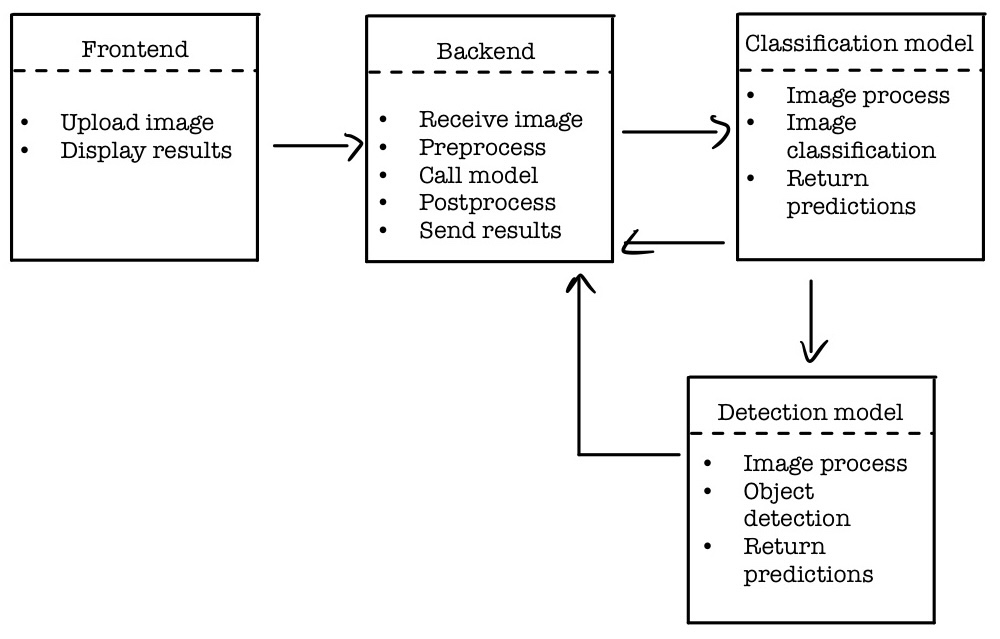
\includegraphics[width=0.5\linewidth]{figures/Figure50.png}
    \caption{System architecture diagram}
    \label{fig:fig38}
\end{figure}

\begin{figure}[H]
    \centering
    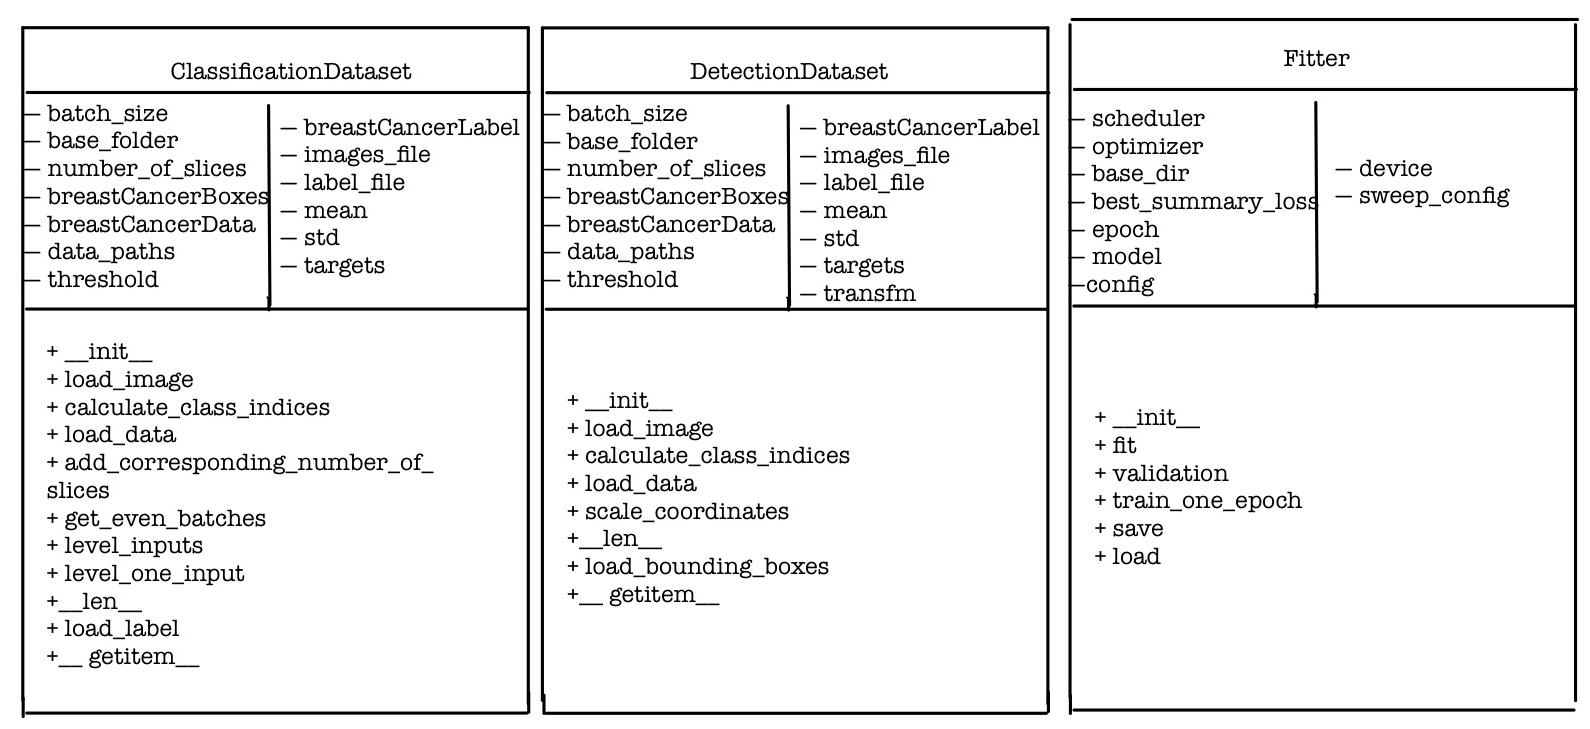
\includegraphics[width=0.5\linewidth]{figures/Figure51.png}
    \caption{System class diagram}
    \label{fig:fig39}
\end{figure}

\begin{figure}[H]
    \centering
    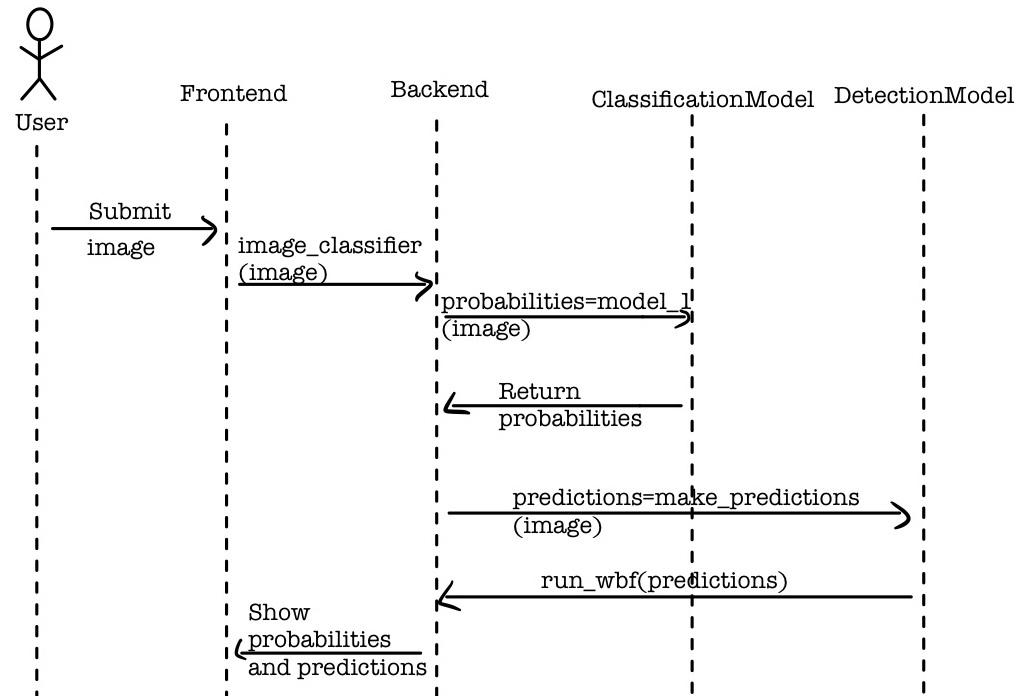
\includegraphics[width=0.5\linewidth]{figures/Figure52.png}
    \caption{System sequence diagram}
    \label{fig:fig40}
\end{figure}

\section{Implementation}
Both the train and front-end section of the system were implemented in Python. For the front-end, I used the library Gradio. First, I used the gradio Interface method of creating a GUI, however I did not like that the examples array was out of view when uploading an image of 512$\times$512. This can be seen in image \ref{fig:fig15}.

\begin{figure}[H]
    \centering
    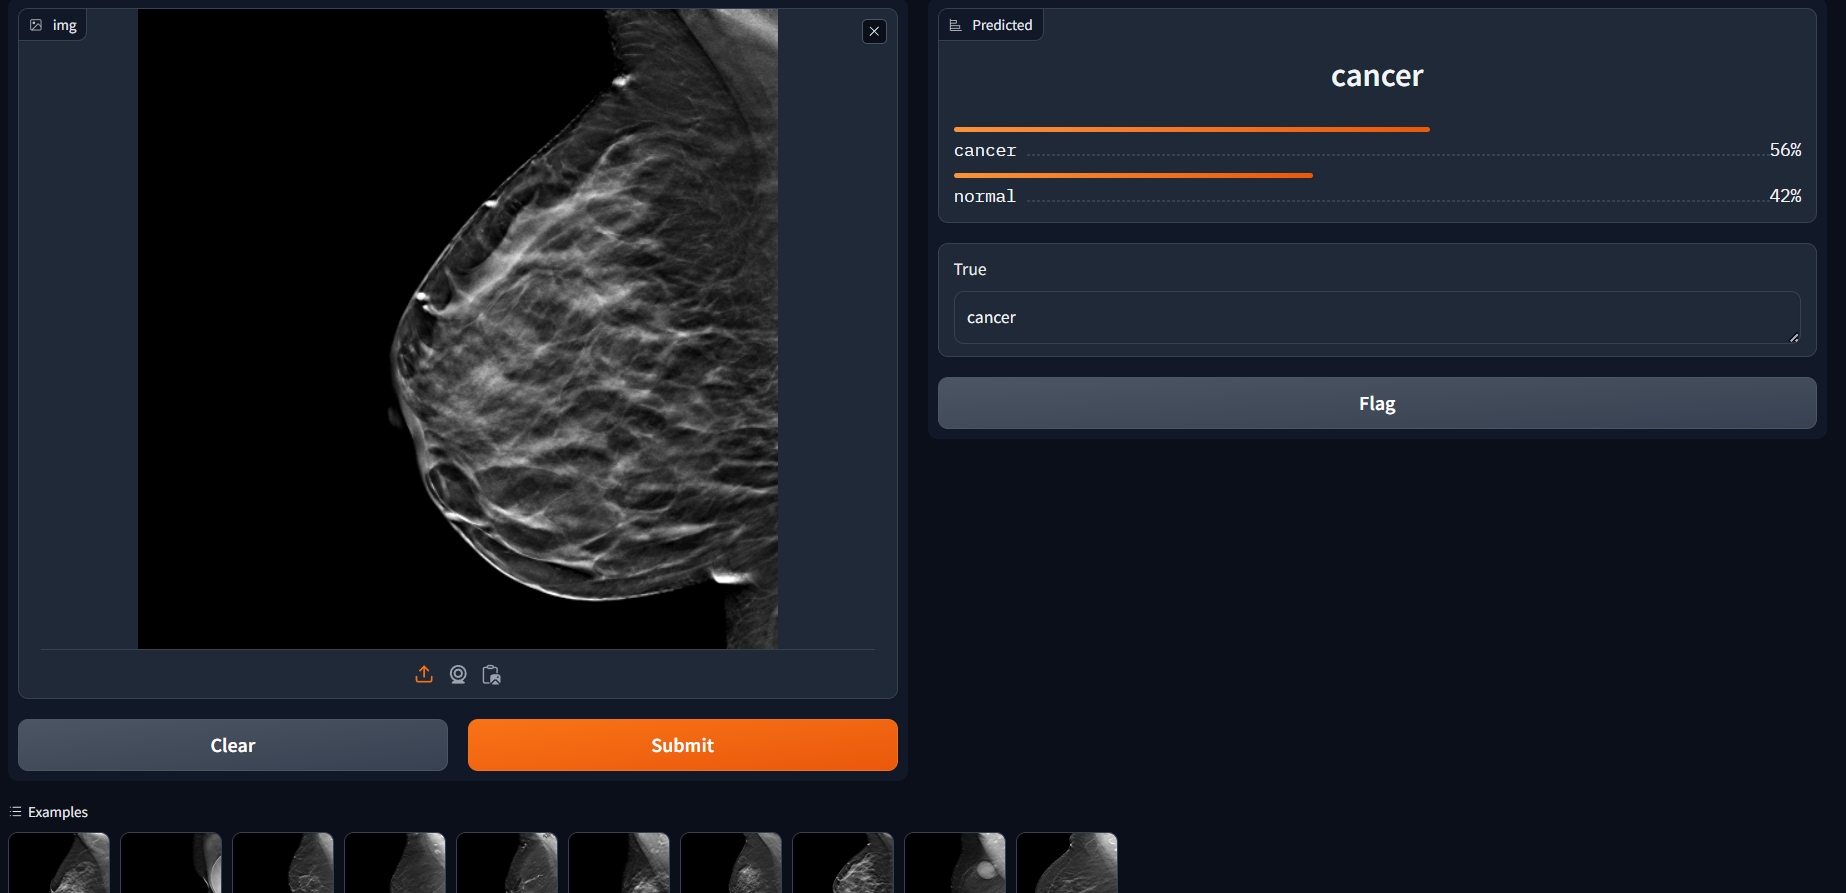
\includegraphics[width=0.75\linewidth]{figures/Figure16.png}
    \caption{Application interface}
    \label{fig:fig15}
\end{figure}

Then, I experimented with the gradio Blocks method and I also chose a theme to go with the system. Figure \ref{fig:fig37} show how the interface looked with no image selected and how it looks like after submitting.

\begin{figure}[H]
    \subfigure[No image selected]{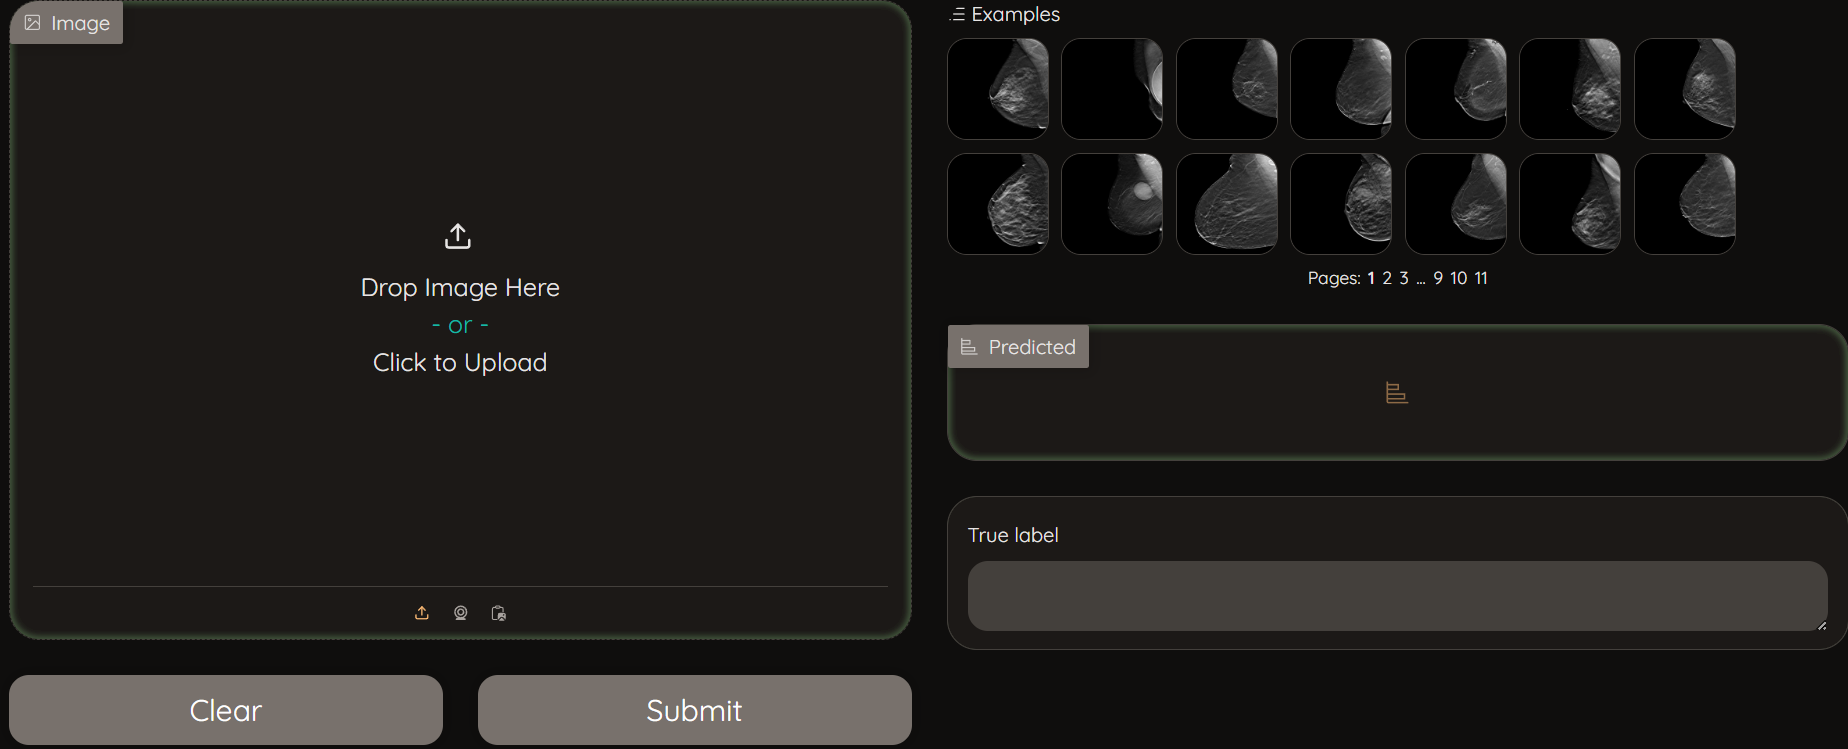
\includegraphics[width=0.5\linewidth]{figures/Figure48.png}}
    \subfigure[Image selected and submitted]{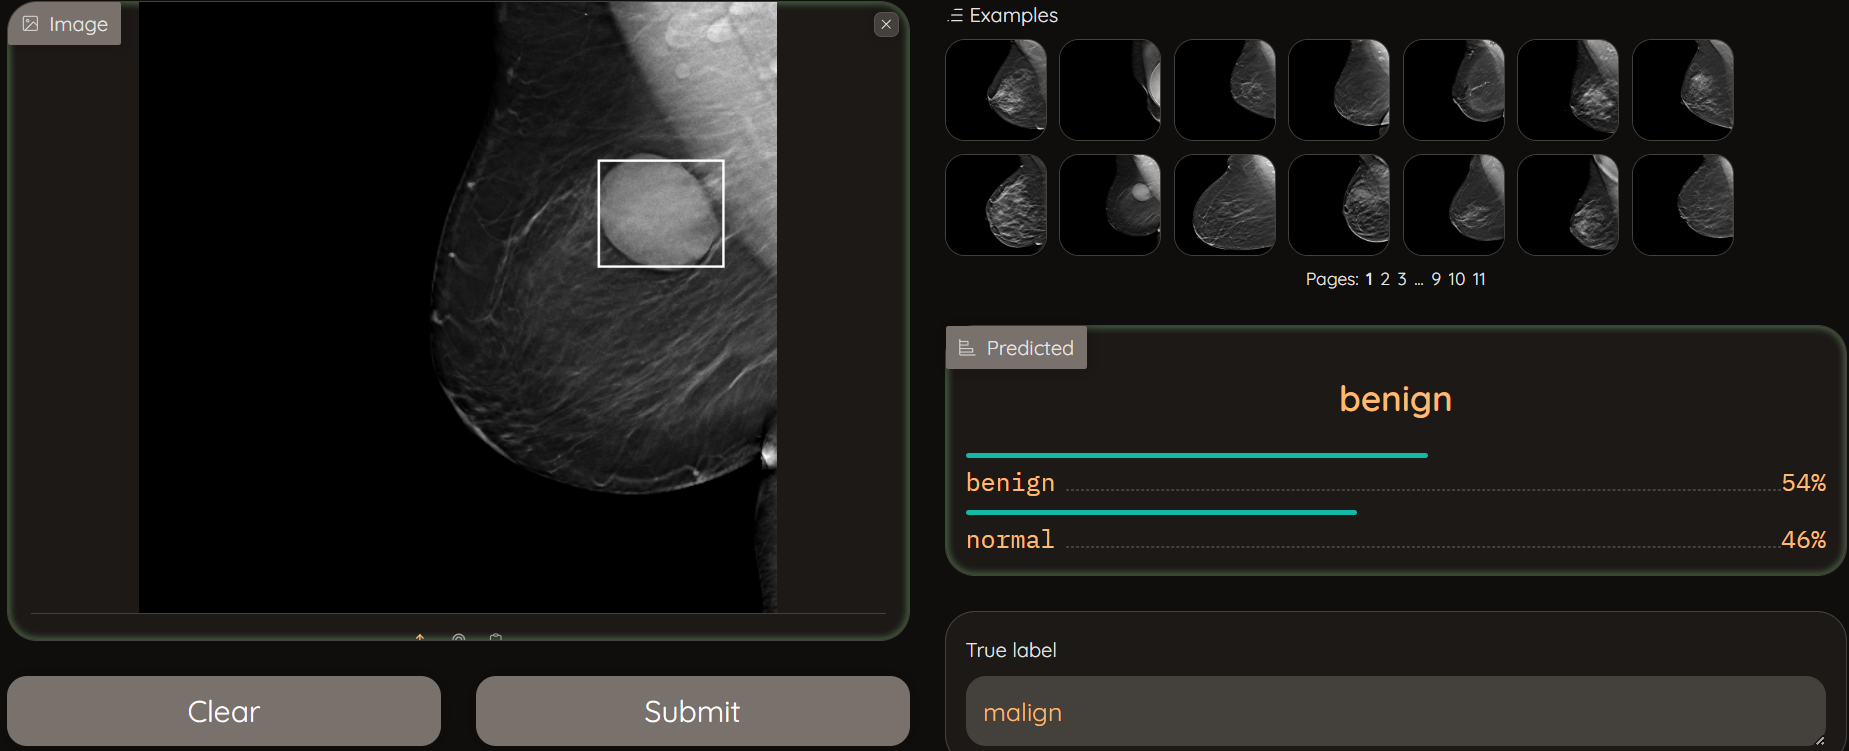
\includegraphics[width=0.5\linewidth]{figures/Figure49.png}}
    \caption{GUI}
    \label{fig:fig37}
\end{figure}

The models' architecture used was the one in the Torch library. I implemented my one datasets for both the classification and detection problems, that inherit methods from \(torch.utlis.data.Dataset\). The order of the inputs so that each batch is balanced is determined directly in the dataset classes, so the \(torch.utils.data.DataLoader\) does not take any sampler classes as input, instead setting the \(shuffle\) attribute to False. The batch size is sent to both the DataLoader and Dataset classes.

\section{Testing and validation}

\textcolor{red}{ar fi bine ca acest capitol sa aiba urm structura:\\
1. fc-nalitati (e.g. load image and detect lessions)\\
2. design (info despre use-case(s), diagrama de arhitectura a app, diagrama de concepte/clase, diagr de secventa)\\
3. implementation (e.g. libraries used,technologies, languages, etc)\\
4. testing and validation (e.g. how you tested the app, some code assertions - it's ok for simple code, not for AI code)\\}
\chapter{Conclusions and possible improvements}
\label{chap:ch6}

The main focus of this thesis is classifying images of digital breast tomosynthesis and detecting the tumors present in the cancerous ones. The classification is achieved by passing 22 slices from each 3D scan, resizing it to $512\times512$, through a GoogLeNet model, which returns an array of 2 values between 0 and 1, representing the probability that the image submitted is normal or cancerous. The model is evaluated both in the train phase, by comparing loss graphs, and also in the test phase, by comparing confusion matrices and computing the accuracy, precision and recall.

The detection is performed in a similar way, meaning that the images are sent as 22 individual slices of size $512\times512$. However, the model returns three values: the array of bounding boxes that might have tumors present, an array of integer values representing the classes, benign or malign that these tumors belong to, and an array of values between 0 and 1 representing the probability of the bounding boxes existing. The loss of these predictions is computed directly in the architecture of the model, both for the train and test losses. Because the test evaluation was done in the form of a loss graph, I did not compute the IoU value of these predictions.

In this thesis, I managed to compare results from different experiments conducted on the GoogLeNet classification model. There have been six experiments and out of all of them, the best model found has an accuracy of 0.6232; precision and recall for cancer images are 0.6694 and 0.4922, respectively. The hyper-parameters for this configuration are: learning rate of 0.0001, Adam optimizer, a Step learning rate decay of step 5 and gamma 0.1.

The six experiments on the detection model proved to be more fruitful, achieving an overall better loss for both test and train losses. The final configuration of these experiments achieved a train loss of 0.8469 maximum and 0.02313 minimum, while the train loss was 1.906 maximum and 1.315 minimum. The hyper-parameters include a learning rate of 0.0001, a CosineAnnealingLR learning rate decay with a minimum of $1e^{-6}$ learning rate, called after each batch of size 16 in the dataset.

As for the possible improvements, GoogLeNet proved to not be a worthy architecture for the classification of cancer tumors in digital breast tomosynthesis images because of the low accuracy obtained. I propose a different architecture, maybe DenseNet or ResNet to train and compare the results obtained by GoogLeNet. Additionally, I would increase the length of the dataset even more by including all the slices, keeping in mind the risk that some inputs might overpower others, especially considering the fact that the lowest number of slices an image has in the database is 22, and the highest number is 120.

However, for the EfficientDet model, I am quite happy with the results of the trained model. I would maybe experiment with other types of EfficientDet, from D1 to D5. I do have some concerns, mainly the fact that the test loss seems to slightly increase from epoch to epoch while the train loss decreases. While the CosineAnnealing learning rate decay proved to work well with the model, I would experiment with other types of learning rate decay, such as OneCycle.

\section{SWOT Analysis}

The SWOT analysis presented in the image \ref{fig:fig44} identifies the strengths, weaknesses, opportunities, and threats for my MammoDetect system.

\begin{figure}[H]
    \centering
    \includegraphics[width=0.5\linewidth]{figures/Figure54.png}
    \caption{SWOT analysis}
    \label{fig:fig44}
\end{figure}

\textbf{Strengths}:
The project benefits from the expertise of a professor in artificial intelligence, providing valuable guidance. I have access to university resources and facilities, such as libraries, as licenses. I used existing technologies but applied them innovatively, which can provide competitive advantages.

\textbf{Weaknesses}:
I have limited experience in the healthcare sector, which can affect my understanding and correct approach to specific problems. The project has a strict deadline, which can create pressure and impact the quality of work. Financial resources are limited, restricting the ability to invest in advanced technologies or necessary equipment.

\textbf{Opportunities}:
There is a growing interest in digital health solutions, especially for diseases that predominantly affect women, offering a target market. There is an increasing demand for remote monitoring solutions, which can create opportunities for the adoption of the technology developed by the project.

\textbf{Threats}:
Strict data protection regulations can create obstacles in the collection and management of patient data. Technology evolves rapidly, which can make the solutions developed quickly outdated. There are already other AI-based tumor detection applications on the market, creating significant competition.



\bibliography{references}

\end{document}
